\documentclass[9pt]{beamer}

\mode<presentation>
{
  \usetheme{Pittsburgh}
  \usecolortheme{dolphin}
  \setbeamercovered{transparent}
  %\setbeamertemplate{footline}[default]
    %\setbeamertemplate{footline}[frame number]
  \setbeamertemplate{navigation symbols}{}
	\usefonttheme{professionalfonts}
}


\usepackage[english]{babel}
\usepackage[latin1]{inputenc}
\usepackage{times}
\usepackage[T1]{fontenc}
\usepackage{csquotes}
\usepackage{amsmath}
\usepackage{amsthm}
\usepackage{amsfonts}
\usepackage{amssymb}
\usepackage{mathtools}
\usepackage{framed}
\usepackage[square]{natbib}
\usepackage{graphicx}
\usepackage{media9}

\newcommand{\pp}{\pause}
%\newcommand{\pp}{ }
\newcommand{\vsk}{\vspace{0.1cm}}

\newcommand{\prob}{\mathbb{F}}
\newcommand{\finfo}{\mathcal{F}}
\newcommand{\ex}{\text{E}}
\newcommand{\vr}{\text{Var}}
\newcommand{\crr}{\text{Corr}}
\newcommand{\rnQ}{\mathbb{Q}}
\newcommand{\forward}{\text{For}}
\newcommand{\future}{\text{Fut}}
\newcommand{\variance}{\mathbb{V}\text{ar}}
\newcommand{\indicator}{\mathbb{I}}
\DeclareMathOperator*{\argmax}{arg\,max}

\newcommand{\approxtext}[1]{\ensuremath{\stackrel{\text{#1}}{\approx}}}

\newcommand\Fontvi{\fontsize{6}{7.2}\selectfont}
\newcommand\Fontviii{\fontsize{8}{7.2}\selectfont}


\setbeamerfont{page number in head/foot}{size=\small}
\setbeamertemplate{footline}[frame number]



\title
{Fintech and Cryptocurrencies}
\author[Co-Pierre Georg]
{
Co-Piere Georg\footnote{These slides are published under the \href{https://www.gnu.org/licenses/lgpl-3.0.en.html}{Gnu LGPL v3.0 license}. Developed in collaboration with Qobolwakhe Dube. Please contact me under \url{cogeorg@gmail.com} if you have any comments or find mistakes in these slides. Perpetual work in progress.}\\
University of Cape Town
}
%\institute[University of Cape Town]{ACQuFRR Seminar Series \\  University of Cape Town}
\date
{This version: 2018-01-16}


\begin{document}

\begin{frame}
  \titlepage
\end{frame}

% -----------------------------------------------------------------

\section{Fintech}

\begin{frame}{What is fintech?}
	\begin{itemize}
		\item The use of technology and other innovations to support or enable the delivery of banking and other financial services
		\item The term has come to collectively represent technologies that are disrupting traditional financial services, including mobile payments, money transfers, loans, fund raising, and asset management
		\item This technology is being used to develop innovative ways of producing and consuming financial products and services that can meet consumer needs more efficiently or cheaply
	\end{itemize}
\end{frame}

% -----------------------------------------------------------------
\subsection{Digital disruption}

\begin{frame}{Digital disruption}
	The \href{https://hbr.org/2015/12/what-is-disruptive-innovation}{Harvard Business Review} describes "Disruption" as a process whereby a smaller company with fewer resources is able to successfully challenge established incumbent businesses \\ \vspace{3mm}
	Disruptive innovations originate in low-end or new-market footholds
	\begin{itemize}
		\item Established firms typically provide and innovate for their most profitable and demanding customers segments, paying less attention to less-demanding customers, creating an opportunity for new entrants
		\item Alternatively disrupters create a market where none existed as they find a way to turn non-consumers into consumers
	\end{itemize}
\end{frame}

% -----------------------------------------------------------------

\begin{frame}{Digital disruption}
	\begin{figure}[]
		\centering
		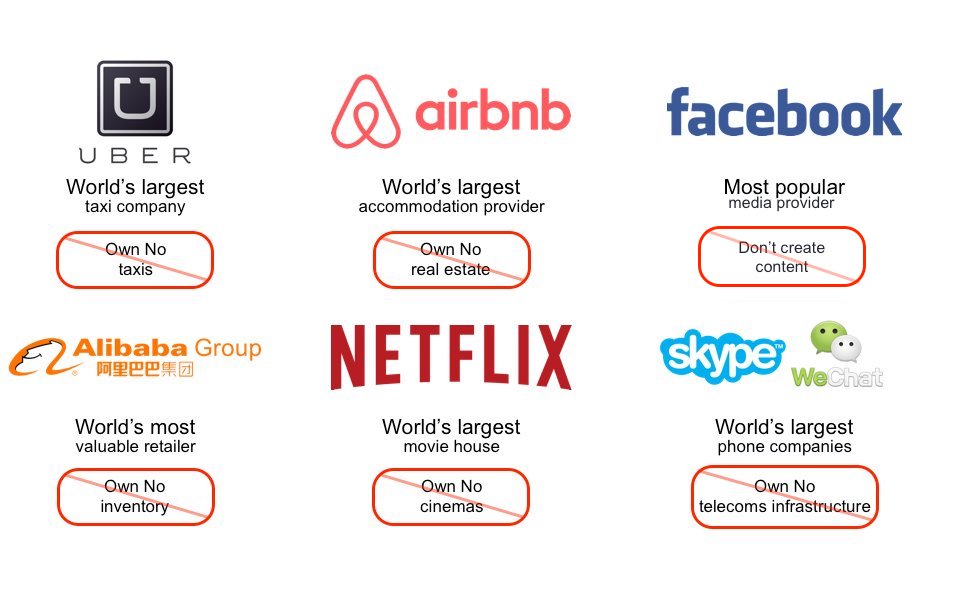
\includegraphics  [scale=0.3]{Images/disruption}
	\end{figure}
\end{frame}

% -----------------------------------------------------------------

\begin{frame}{Digital disruption}
	According to PricewaterhouseCoopers' \href{http://www.pwc.com/ee/et/publications/pub/pwc-global-fintech-report-2017.pdf}{2017 Global FinTech Report}, large financial institutions across the world could lose 24 percent of their revenues to fintech companies over the next three to five years\\ \vspace{3mm}
	A Citigroup report published in 2016 warned that European and American banks could lose almost 2 million jobs in the next 10 years \\ \vspace{3mm}
	A report by \cite{buchak2017} for the National Bureau of Economic Research found that fintech firms accounted for roughly a quarter of shadow bank loan origination in 2015, partially benefiting from their online origination technology \\ \vspace{3mm}
\end{frame}

% -----------------------------------------------------------------

\begin{frame}{Global investment}
	Investment in fintech has grown from \$1.8 billion in 2010 to \$19 billion in 2015, and in 2015, its estimated market worth was about \$4.7 trillion, according to Goldman Sachs \\ \vspace{3mm}
	In 2016 the total value of investment in fintech among the top 10 countries by deal value accounted for 95\% of global investment \\ \vspace{3mm}
	KPMG reported that the top 10 largest deals of 2017 occurred in the United States, China, Germany and Canada
\end{frame}

% -----------------------------------------------------------------

\begin{frame}{Global investment}
	\begin{figure}[]
		\centering
		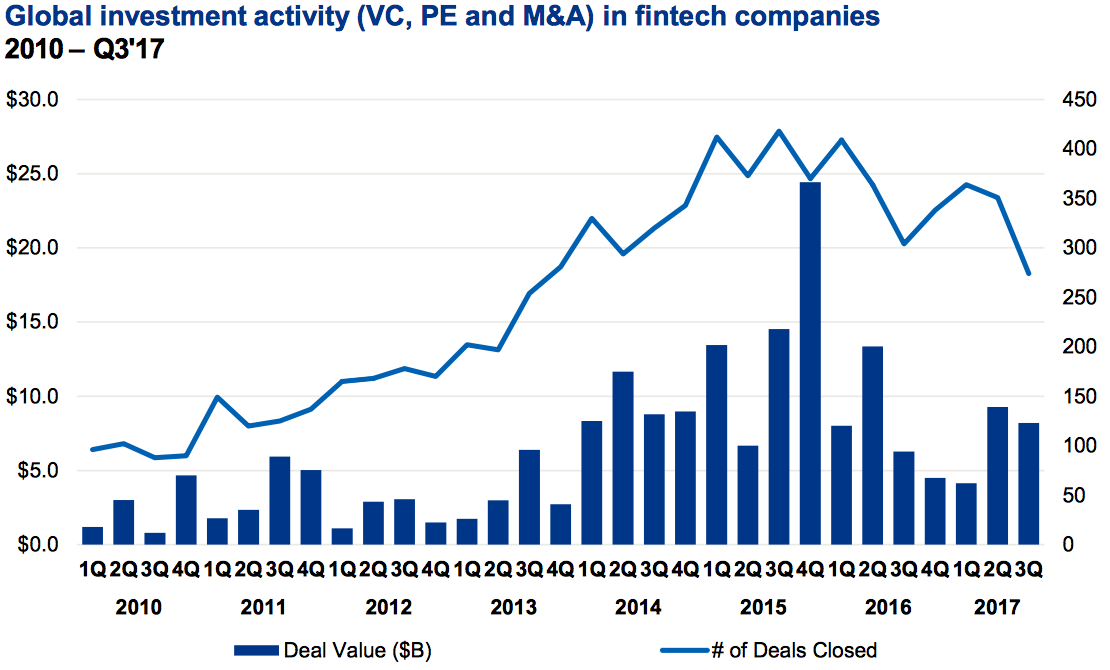
\includegraphics  [scale=0.2]{Images/kpmg}
	\end{figure}
	\begin{tiny}
		Source: \href{https://home.kpmg.com/za/en/home/insights/2017/11/the-pulse-of-fintech-q3-2017-.html}{KPMG: The Pulse of Fintech Q3 2017}
	\end{tiny}
\end{frame}

% -----------------------------------------------------------------

\begin{frame}{Disrupting finance}
	Why is fintech so important?
	\begin{itemize}
		\begin{small}
			\item These innovations are not just changing the competitive patterns within the industry but are leading a paradigm shift in the way in which industry operates and services its customers
			\begin{itemize}
				\item The emphasis on peer to peer interaction  challenges the role of traditional intermediaries in the financial markets
				\item Many of these innovations harness the ability to transact in real time through low cost payment channels
				\item The ability to conduct real time analysis of the market has the potential to improve the efficiency of regulatory functions
				\item Fintech further addresses frictions that come as a result of information asymmetries by making information more accessible
			\end{itemize}
		\end{small}
	\end{itemize}
\end{frame}

% -----------------------------------------------------------------

\begin{frame}{Disrupting finance}
	\begin{itemize}
		\item The rapid emergence of new service providers offering solutions based on these technologies is changing the financial ecosystem
		\item Some traditional financial institutions are responding by transforming their own operations, either by adopting similar technologies or collaborating with fintech companies
		\item At its core, fintech has the potential to
		\begin{itemize}
			\item Empower customers who will be able to deal directly, more seamlessly, and flexibly with product and service providers
			\item Empower businesses to deliver a better value proposition and customer experience to their customer base
		\end{itemize}
	\end{itemize}
\end{frame}

% -----------------------------------------------------------------

\begin{frame}{Key drivers}
	\begin{figure}[]
		\centering
		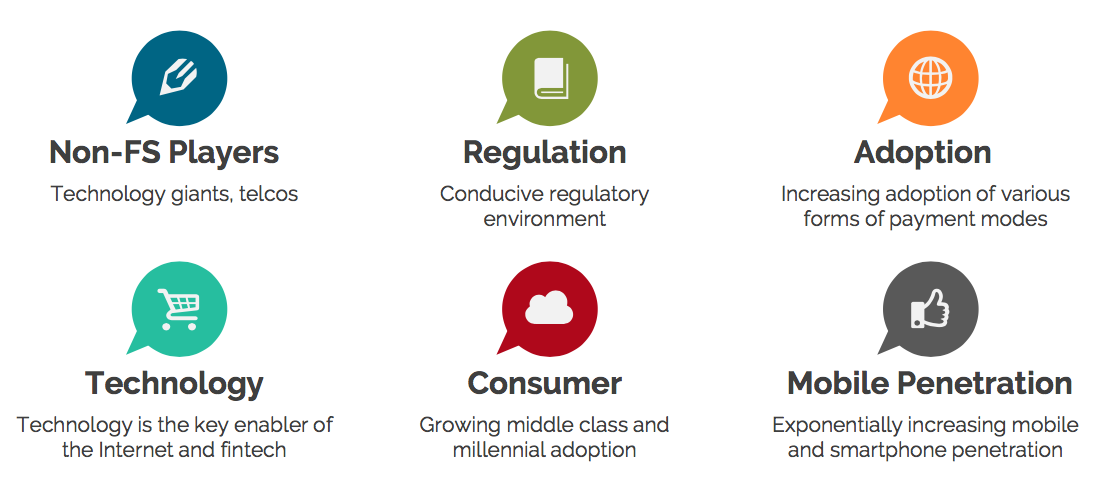
\includegraphics  [scale=0.5]{Images/drivers}
	\end{figure}
	\begin{tiny}
		Source: \href{https://www.slideshare.net/JoeSeunghyunCho/fintech-in-asia-epayments-marvelstone-tech-at-sgx-event}{https://www.slideshare.net/JoeSeunghyunCho/fintech-in-asia-epayments-marvelstone-tech-at-sgx-event}
	\end{tiny}
\end{frame}

% -----------------------------------------------------------------

\begin{frame}{Financial inclusion}
	\begin{itemize}
		\item According to the World Bank, the number of people globally with no access to banking and financial services is almost two billion
		\item There are many reasons for this, including
		\begin{itemize}
			\item Insufficient credit history
			\item Bad credit history
			\item Limited access to credit and other financial services
		\end{itemize}
	\end{itemize}
\end{frame}

% -----------------------------------------------------------------

\begin{frame}{Financial inclusion}
	\begin{itemize}
		\item These advances in technology are poised to make financial services accessible for the un-banked
		\begin{itemize}
			\item Access is no longer restricted by geographical location or other physical barriers
			\item Services become more affordable as institutions pass on reduced costs to customers
		\end{itemize}
		\item Digital platforms further improve the personalization of services and lead to more relevant product offerings
		\item The spread of mobile technologies and mobile network coverage has driven the interest in mobile based financial services
	\end{itemize}
\end{frame}

% -----------------------------------------------------------------

\begin{frame}{Mobile penetration}
	\begin{itemize}
		\item Relative to developed economies, fintech investment is low, however Africa is often seen at the forefront of mobile financial innovation
		\item Access to digital services has largely been supported by the mobile phone. A 2017 report by Ericsson found that Sub Saharan Africa has the highest growth rate in mobile subscriptions globally
		\item South Africa has been ranked as the most developed digital economy in Africa
		\begin{itemize}
			\item Mobile phone penetration exceeds 90\% of the adult population with 69\% using smartphones
			\item Internet penetration has been rising steadily from 46\% in 2015 to 52\% in 2017
		\end{itemize}
	\end{itemize}
\end{frame}

% -----------------------------------------------------------------

\begin{frame}{Digital Innovation}
	\begin{itemize}
		\item Innovation is occurring across the financial services industry
		\begin{itemize}
			\item Distributed ledger technologies are being as new ways for structuring market infrastructures and payment services. The market for payments is often the most attractive area for innovation as it is typically the least regulated banking function
			\item Transaction data and artificial intelligence are being leveraged for credit appraisals
			\item The markets for deposits, lending and capital raising are seeing an increase in peer to peer activity and crowdfunding
			\item In the field of investment management, advances are being made in the automated precessing and dissemination of investment advice
		\end{itemize}
	\end{itemize}
\end{frame}
% -----------------------------------------------------------------

\begin{frame}{Payments}
	\begin{itemize}
		\item This function has seen advances both within and outside the traditional payment infrastructure and channels
		\item The development of smartphone payments and card-based payment platforms by streamlining electronic fund transfer (EFT) payments has led to a shift toward non-cash channels
		\item These developments are being supported by next generation security measures such as location-based identification and biometrics, which protect customers and increase confidence in digital channels
		\item Outside of the traditional payment channels, has empowered consumers to securely transfer value with limited transaction costs, near real time settlement and without the need for intermediaries
	\end{itemize}
\end{frame}

% ------------------------------------------------------------------

\begin{frame}{Deposits and lending}
	\begin{itemize}
		\item This banking function is being disrupted by innovation particularly in the credit market and in the way customers are being serviced
		\item New service providers are emerging, offering alternative ways to assess credit and secure funding for lending products outside of the banking system
		\item Crowd-based funding platforms to secure funding for lending are gaining popularity, and in some instances passing the risk to the investors
		\item Furthermore, traditional financial intermediaries are being eliminated in some instances by the rise in peer-to-peer lending.
	\end{itemize}
\end{frame}

% ------------------------------------------------------------------

\begin{frame}{Capital markets}
	\begin{itemize}
		\item  Alternative funding platforms have begun to emerge, which allow individuals and start-ups to source funding from a collection of investors directly through an online market place, i.e. crowdfunding
		\item There are four forms of crowdfunding
		\begin{small}
			\begin{enumerate}
				\item Donations-based funding - provided on a charitable basis without any expectation of a reward
				\item Reward-based - provides an item of clear monetary value in exchange for the funding provided
				\item Loan-based - investors expect to earn interest and capital repayments on the amount funded i.e. peer-to-peer lending
				\item Investment-based - funding provided to earn capital gains and dividends.
			\end{enumerate}
		\end{small}
		\item These platforms continue to increase in popularity as they can also provide investors with access to a far wider array of investment opportunities not bounded by geography
		\item It also becomes easier to give investors more control over where and how their funds are invested
	\end{itemize}
\end{frame}

% ------------------------------------------------------------------

\begin{frame}{Investment management}
	\begin{itemize}
		\item Technology enabled solutions are being used to provide advice, market information and easy to use investment tools.
		\begin{itemize}
			\item Robo-advisors are being used to administer advisory services and guide investors' decisions in the absence of human oversight.
			\item Platforms are being designed to give investors the ability to automate trade execution, based on a predefined set of rules and automated quantitative investment strategies
			\item Investment managers' administrative processes can be automated and streamlined through the use of artificial intelligence and in so doing reduce the likelihood of human error
		\end{itemize}
		\item These factors all contribute towards efficiencies and reduced costs passed on to consumers, consequently making investment products more affordable and attractive.
	\end{itemize}
\end{frame}

% ------------------------------------------------------------------

\begin{frame}{Market microstructure}
	\begin{itemize}
		\item Markets are seeing a rise in high frequency trading strategies (i.e. exploiting arbitrage opportunities through low-latency access to exchanges) being supported by big data analytics and artificial intelligence
		\item Algorithms make use of new machine-readable data sources and AI capabilities, providing traders with the opportunity to react to real time events more quickly, in so doing providing the market with liquidity
		\item Technology is also changing the way in which buyers and sellers connect in the OTC market
		\item In many ways, the OTC market is being formalized without necessarily involving financial intermediaries
		\item These platforms being used to connect market participants are providing the opportunity for greater price transparency and improved liquidity
	\end{itemize}
\end{frame}

% ------------------------------------------------------------------

\begin{frame}
	\begin{figure}[]
		\centering
		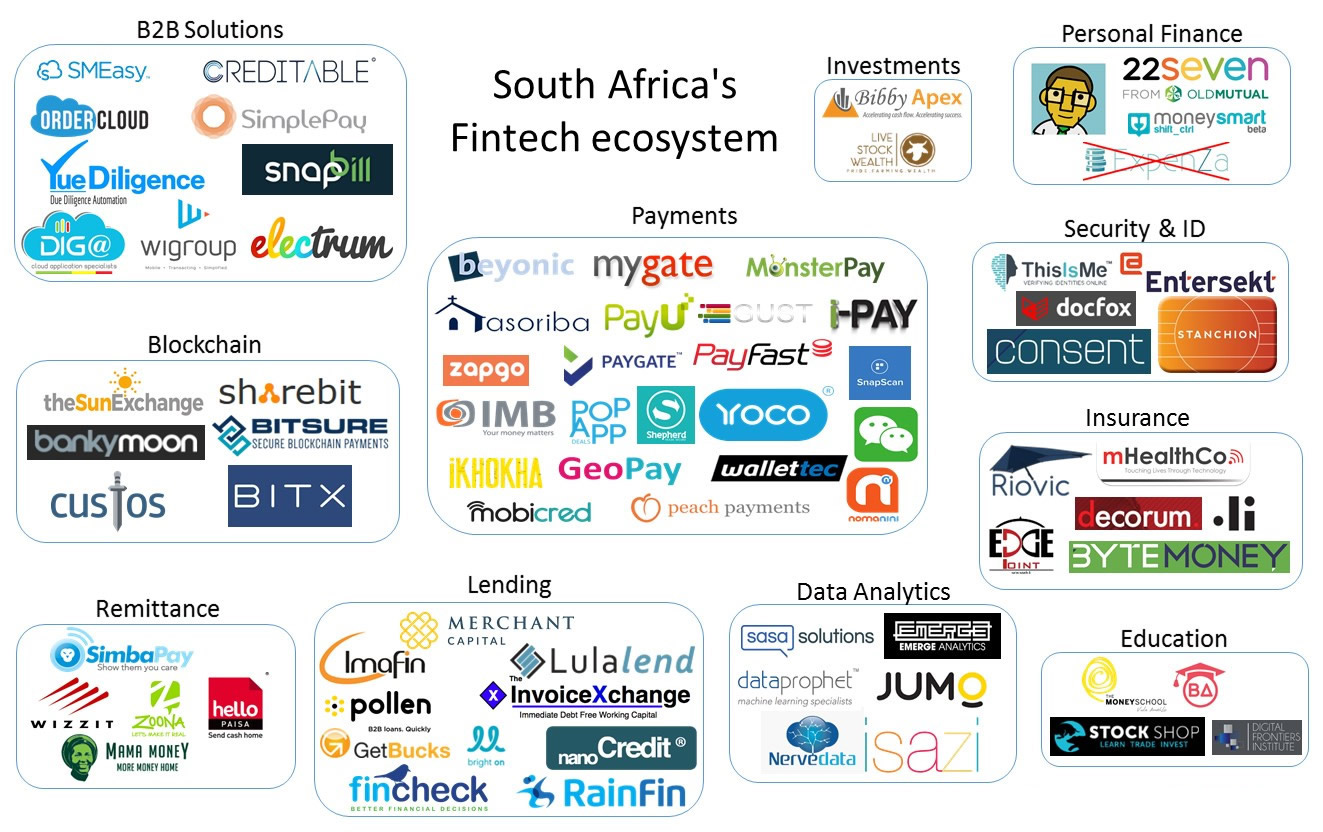
\includegraphics  [scale=0.2]{Images/ecosystem}
	\end{figure}
	\begin{tiny}
		Source: \href{http://ventureburn.com/2016/09/uncovered-ventureburn-lists-south-africas-fintech-ecosystem/}{http://ventureburn.com/wp-content/uploads/2016/09/uncovered-ventureburn-lists-south-africas-fintech-ecosystem-update-01.jpg}
	\end{tiny}
\end{frame}

% ------------------------------------------------------------------

\subsection{Fintech in action}

\begin{frame}{Fintech in action}
	Digital payments
	\begin{itemize}
		\item \href{https://www.google.com/wallet/}{Google wallet} - Mobile application that digitizes users' cards to facilitate P2P and P2P payments online and at points of sale
		\item \href{www.wigroupinternational.com}{WiGroup} - Started off as the first mobile wallet in SA in 2008, and has since evolved into a facilitator of mobile transaction services.
		\item \href{http://www.snapscan.co.za}{Snapscan} - A pay-by-proxy allowing businesses to accept card transactions with mobile phones
		\item \href{https://masterpass.com}{MasterPass} A mobile application digitizing users' cards allowing payment through QR codes and online
	\end{itemize}
\end{frame}

% -----------------------------------------------------------------


\begin{frame}{Fintech in action}
	Smartphone payments
	\begin{itemize}
		\item \href{https://www.yoco.co.za/}{Yoco} - Mobile payments service provider that targets small to medium companies who require the portability of a card reader. In the past two years of operation, raised US\$7 million
		\item \href{https://www.apple.com/apple-pay/}{Apple pay} A mobile wallet with NFC enabled capabilities allowing for P2P and contactless POS payments
		\item \href{http://www.fit-pay.com}{FitPay} - A provider that enables contactless payments through wearable devices
		\item \href{http://cardsplus.co.za}{CardsPlus} - A South African producer and supplier of contactless and contact chip cards
	\end{itemize}
\end{frame}


% -----------------------------------------------------------------

\begin{frame}{Fintech in action}
	Compliance and regulation
	\begin{itemize}
		\item \href{https://www.alyne.com/en/}{Alyne} - a regtech Software as a Service for cyber security, risk management and compliance. Provides scalable assessments to measure current maturity and delivers deep insights through advanced risk analytics.
		\item \href{https://www.bokio.se}{Bokio} - Automates accounting and serves as a decision-making platform for small businesses. The system automatically handles invoicing, payroll and accounting
		\item \href{https://suade.org/}{Suade} - focused on prudential regulation stemming from Basel III and Mifid II, and provides products including a stress testing platform for capital requirements and scenario testing for liquidity management
		\item \href{https://complyadvantage.com}{ComplyAdvantage} - A London based anti money laundering and sanctions database
		\item \href{https://gusto.com/}{Gusto} - A comprehensive HR, payroll, and benefits service, enabling businesses to set up and run payroll from any web-enabled device.
	\end{itemize}
\end{frame}

% -----------------------------------------------------------------

\begin{frame}{Fintech in action}
	Security \& ID
	\begin{itemize}
		\item \href{https://www.entersekt.com}{Entersekt} - Provider of push-based security and authentication, as well as biometric verification. %In 2009, it raised US\$250 000 from Ramzi Mansour and went on to raise an additional US\$9-million from a range of other undisclosed partners
		\item \href{https://www.prosper.com/daily}{Prosper Daily} - A personal finance security company that analyzes users' card based transactions to alert them to potential fraud
		\item \href{https://www.thisisme.com/}{ThisIsMe} - an online verification system or individuals, businesses, regulators, and financial institutions that works by linking into Home Affairs and major banks%. Received US\$2.5million in funding from private investors in 2016
		\item \href{https://www.vcs.co.za/home/home.asp}{Virtual Card Services} - A card payments service provider that offers 3D secure solutions
	\end{itemize}
\end{frame}

% -----------------------------------------------------------------
\begin{frame}{Fintech in action}
	Payment platforms
	\begin{itemize}
		\item Stripe - provides a set of unified APIs and tools that instantly enable businesses to accept and manage online payments
		\item Ant Financial - an online payment services provider Founded by the Alibaba group. Its platform, Alipay, is the world's largest mobile and online payments platform
		\item \href{https://www.shieldpay.com/}{ShieldPay} - Operates an instant digital escrow facility that enables secure Peer-Peer transactions
	\end{itemize}
\end{frame}

% -----------------------------------------------------------------

\begin{frame}{Fintech in action}
	Domestic and international remittances
	\begin{itemize}
		\item \href{https://www.safaricom.co.ke/personal/m-pesa}{M-Pesa} - An agency based mobile money operator based in Kenya that provides money transfer, financing and microfinancing services
		\item \href{https://www.shoprite.co.za/money-market/money-transfers.html}{Shoprite Money Market} - A large South African retailer providing almost instant cash-in cash-out transfers from its branches
		\item \href{https://transferwise.com/}{TransferWise} - An international remittance platform that pairs senders and receivers in local markets
		\item \href{http://sa.mukuru.com}{Mukuru Money} - An international remittance platform that operates through partnership with retailers and banks
	\end{itemize}
\end{frame}

% -----------------------------------------------------------------

\begin{frame}{Fintech in action}
	Blockchains
	\begin{itemize}
		% \item \href{https://www.lu.com}{Lufax} - A online marketplace for the origination and trading of financial assets. Total funding received to date is \$1.7bn
		\item \href{http://blockchain.com/}{Blockchain} - A web-based bitcoin platform that provides Bitcoin wallet services, Bitcoin APIs, and a block explorer
		\item \href{https://www.coinbase.com}{Coinbase} - A digital currency wallet service provider that allows merchants, consumers, and traders to to buy and sell digital currency
		\item \href{https://www.luno.com/en/}{Luno}(formerly BitX) - A digital wallet that allows consumers to easily buy and sell Bitcoin. %In July 2015, the company raised over US\$4-million in funding from Naspers, along with US\$800 000 from investors in late 2014
		\item \href{https://thesunexchange.com/}{The Sun exchange} - A market place where you can buy into commercial solar projects at the scale of one cell at a time, using blockchains and smart contracts to facilitate transactions
	\end{itemize}
\end{frame}


% -----------------------------------------------------------------

\begin{frame}{Fintech in action}
	Insurance
	\begin{itemize}
		\item \href{riovic.com/}{Riovic} - Directly connects risk managers and risk underwriters. It also allows private investors to accept a stream of certain cash flows in exchange for an uncertain future liability.
		\item \href{https://www.robinhoodpro.com}{Robin} - Provides a mobile interface presenting all the present and past retirement and pension funds under your name. Allowing you to monitor the fees you are paying, the ROI, the predicted monthly pension and how much can be saved on fees by upgrading existing plans with better ones
		\item \href{http://www.meetleo.co}{LeO Chief Of Stuff} - Applies Machine Learning and Artificial Intelligence technologies on user's profile and on real-time data, to deliver a optimized insurance experience and match the user with the most relevant insurance products
		\item \href{compsol.co.za/}{eCOIDA} - an online insurance technology platform that links employers and medical service providers
	\end{itemize}
\end{frame}

% -----------------------------------------------------------------


\begin{frame}{Fintech in action}
	Credit facilities
	\begin{itemize}
		\item \href{https://salaryo.com/}{Salaryo} - Provides credit facilities to freelancers with unstable income. The platform verifies the applicant's identity, checks financial health in real time and analyses the freelancer's professional pulse with a proprietary risk management model
		\item \href{www.flexpay.co.ke/}{Flexpay} - Provides an automated purchase platform that enables customers to afford goods via convenient flexible mobile phone payments.
		\item \href{https://fomo.travel/}{FOMO Travel} - An online lay-buy platform where one can pay a small deposit towards a travel goal and pay the rest through installments or crowdfunding. Recently entered into a partnership with SA Tourism
	\end{itemize}
\end{frame}

% -----------------------------------------------------------------

\begin{frame}{Fintech in action}
	Alternative credit scoring
	\begin{itemize}
		\item \href{https://commuscore.com/}{Commuscore} - A South African provider of credit scoring that integrates data from informal social saving and lending groups
		\item \href{https://www.kreditech.com}{Kreditech}  - A German online lender which offers loans to individuals based on their creditworthiness which is analyzed using their social media and online data
		\item \href{https://www.compuscan.co.za}{Compuscan} - A credit bureau integrating psychometric data into credit scoring
	\end{itemize}
\end{frame}
% -----------------------------------------------------------------


\begin{frame}{Fintech in action}
	Asset financing
	\begin{itemize}
		\item \href{ownerhood.co/en/}{Ownerhood} - By breaking properties into smaller tradeable slices Ownerhood removes barriers to homeownership and promotes frictionless access to the residential real-estate market via a simple, digital, crowd driven marketplace
		\item \href{benben.com.gh/}{BenBen} - A digital land database that provides fast and easy access to trusted information about land through Blockchain technology. Provides access to paid-for-property information, mortgage origination, licensing, thematic data analysis.
		\item \href{http://www.carvana.com/}{Carvana} -  A online platform that enables users to trade, finance, buy, and sell used cars using a fully-automated service scheme
		\item \href{http://www.gotugende.com}{Tugende} - A Ugandan platform allowing users to finance and payoff a motorcycle in 18 months or less
	\end{itemize}
\end{frame}

% -----------------------------------------------------------------

\begin{frame}{Fintech in action}
	Peer-to-peer lending
	\begin{itemize}
		\item \href{https://www.lendingclub.com}{Lending Club} - A US provider of peer to peer unsecured personal loans of up to \$40,000
		\item \href{https://www.upstart.com}{Upstart} - An online lending marketplace that provides personal loans using alternative scoring methods, like education and employment, to predict creditworthiness
		\item \href{https://www.rainfin.com/}{RainFin} - An online lending marketplace that connects borrowers seeking transparent, cost effective loans with lenders. It uses an 'intelligent' scorecard to review the applicant's transaction history, financial health, and other aspects such as social media profiles.
		\item \href{http://stokfella.com}{Stokfella} - A digitized social lending and savings platform
		\item \href{http://www.firstp2p.com/}{Firstp2p} -  A Chinese online peer to peer financing site that matches borrowers with investors
	\end{itemize}
\end{frame}

% -----------------------------------------------------------------

\begin{frame}{Fintech in action}
	Automated advice and investment management
	\begin{itemize}
		\item \href{www.kapitalwise.com/}{KapitalWise} - A cost-effective micro-investment platform for financial institutions. Delivers personal investing literacy, rule-based micro investing empowered by machine learning and predictive analytics to retail users of financial institutions
		\item \href{https://www.easyequities.co.za}{Easy Equities} - Provides a low cost web based stock trading platform that allows investors to purchase $1/1000^{th}$ of a share on the JSE
		\item \href{https://www.wealthmigrate.com/za}{Wealth Migrate} - An online platform that allows domestic investors to invest in foreign real-estate developments
		\item \href{https://www.wealthfront.com}{Wealth Front} - An automated investment service firm providing robo-advice reflecting investors' observed financial behavior
	\end{itemize}
\end{frame}

% -----------------------------------------------------------------

\begin{frame}{Fintech in action}
	Banking and Micro-finance
	\begin{itemize}
		\item \href{https://www.abe.ai/}{Abe.ai} - Designs artificial intelligence solutions for the banking industry, helping banks better engage and support their customers at scale
		\item \href{https://www.nomanini.com/}{Nomanini} - Payments platform provider that optimizes transactions in the informal retail sector. Selected as as one of four finalists in the financial inclusion category of the MIT Inclusive Innovation Challenge
		\item\href{www.bytemoney.co.za/}{Byte Money} - Provides solutions that help avoid mismanagement of payments in the informal finance sector with the ability to service remote areas with real time payments
		\item \href{www.kapitalwise.com/}{KapitalWise} - A cost-effective micro-investment platform for financial institutions. Delivers personal investing literacy, rule-based micro investing empowered by machine learning and predictive analytics to retail users of financial institutions
	\end{itemize}
\end{frame}

% -----------------------------------------------------------------

\begin{frame}{Recap}
	\begin{itemize}
		\item Fintech is the use of technology to support delivery of financial services
		\item With the advent of blockchain technology, this sector has seen a significant increase in investment flows
		\item The disruption caused blockchain technology spans across a wide range of functions within financial services
		\item Mobile phone penetration has been found to be one of the key drivers of the adoption of technology in financial services
		\item Banks and other financial institutions face the biggest risk of disintermediation in the functions of payments and investment management
	\end{itemize}
\end{frame}

% -----------------------------------------------------------------

\section{Blockchains}

\begin{frame}
\begin{center}
\begin{large}
Blockchains
\end{large}
\end{center}
\end{frame}

% -----------------------------------------------------------------

\begin{frame}
	\begin{figure}[]
		\centering
		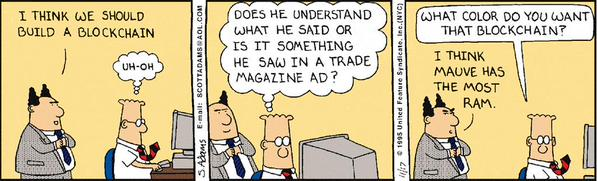
\includegraphics  [scale=0.5]{Images/dilbert-chain}
	\end{figure}
\end{frame}
% -----------------------------------------------------------------

\begin{frame}{}
	\begin{itemize}
		\item Blockchains are a new type of data structure that allows data to be stored on a peer to peer network
		\item Consensus mechanisms are used to determine the contents of the database, which are secured using a combination of cryptographic techniques
		\item Together, the features of transparency, immutability and consensus allow peers to transact in an environment of conflicting interests without the need for trust
		\item Blockchains are expected to revolutionize record keeping practices in the financial sector
		\item This technology can be leveraged for use in virtually any field hat requires the storage of information
	\end{itemize}
\end{frame}

% ------------------------------------------------------------------
\subsection{History of bookkeeping}

\begin{frame}{History of bookkeeping}
	Double entry bookkeeping revolutionized the field of financial accounting during the Renaissance period; it solved the problem of managers knowing whether they could trust their own books \\ \vspace{3mm}
	It has since become the basic foundation of how value is accounted for\\ \vspace{3mm}
	However, due to its complexity, the task of ensuring trustworthiness of records in financial markets is best left to a central authority.
	\begin{itemize}
		\item This makes it easier to deal with high transaction volumes as it if far more efficient to maintain a central ledger where all transactions can be reconciled
		\item It also increases efficiency and reduces the cost of transactions e.g. banks reduce search costs for depositors looking to earn interest and lenders looking for finance
	\end{itemize}
\end{frame}

% -----------------------------------------------------------------

 \begin{frame}{History of bookkeeping}
 	\begin{columns}
 	    \column{0.5\textwidth}
 	    Single entry bookkeeping
 	    \begin{itemize}
 	    	\item Each financial transaction is a single entry in a journal or transaction log
 	    	\item Firms using single entry approach are effectively limited to reporting on a cash basis.
 	    	\item Provides insufficient records and control for public companies and other organizations that must publish audited financial statements
	    \end{itemize}
 	    \column{0.5\textwidth}
 	    Double entry bookkeeping
 	    \begin{itemize}
 		    \item Every financial event brings at least two equal and offsetting entries
 		    \item Firms using the double entry approach report financial results with an accrual reporting system
 		    \item Provides several forms of error checking that are absent in a single entry system e.g. Balance sheet equation
 	    \end{itemize}
 	\end{columns}
 \end{frame}


% -----------------------------------------------------------------

% \begin{frame}{Double entry bookkeeping in legacy banking}
% 	\begin{figure}[]
% 		\centering
% 		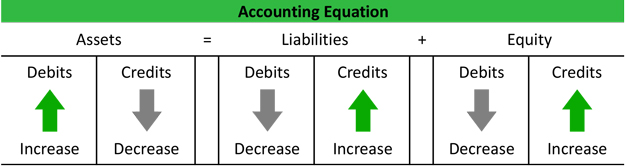
\includegraphics  [scale=0.5]{double-entry}
% 	\end{figure}
% \end{frame}

% % -----------------------------------------------------------------

% \begin{frame}{Double entry bookkeeping in legacy banking}

% \end{frame}

% -----------------------------------------------------------------

\subsection{Blockchain 101}

\begin{frame}{Blockchain}
	The latest innovation that has been posited to disrupt the fintech space is the \textit{blockchain} \\\vspace{3mm}
	This technology offers a new form of storage, use, maintenance and control of records \\\vspace{3mm}
	It has garnered interest not only because of the potential impact on how financial intermediaries will transact with society, but also because of the effect of its application in processes complementary to these financial transactions\\\vspace{3mm}
	This includes but not limited to:
	\begin{itemize}
		\item Identity management
		\item Civil registries of land and asset ownership
		\item Protection of customer privacy
	\end{itemize}
\end{frame}

% -----------------------------------------------------------------

\begin{frame}{What is a blockchain?}
	A distributed database, that records transactions and ownership, operated within a peer to peer network\\ \vspace{3mm}
	Designed to serve as irreversible and incorruptible repositories of information; a digital platform that stores and verifies the entire history of transactions between users across the network. \\ \vspace{3mm}
	Instead of using double entry and keeping separate records based on transaction receipts, the technology allows parties to write their transactions directly into a joint ledger, eliminating the need for a trusted intermediary and creating an interlocking system of enduring records \\ \vspace{3mm}
\end{frame}

% -----------------------------------------------------------------

\begin{frame}
	\begin{figure}[]
		\centering
		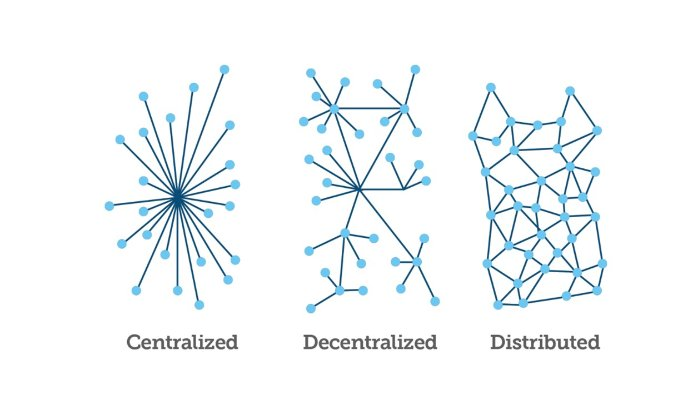
\includegraphics  [width=4.in]{Images/database}
		\begin{centering}
			\caption{A comparison of database network topologies. With both centralized and decentralized networks, nodes retrieve data from a central location, the only difference being that a centralized network has a single point of failure. Whereas with the distributed database architecture, all nodes act as peers, all maintaining local copies of the database, the contents of which are determined by a consensus protocol}
		\end{centering}

		\begin{tiny}
		Source: \href{https://www.businessinsider.com.au/what-is-blockchain-2016-3}{https://static.businessinsider.com/image/56d9fcaf2e52651c008bb97b/image.jpg}
	\end{tiny}
	\end{figure}
\end{frame}

% -----------------------------------------------------------------

\begin{frame}
	\begin{figure}[]
		\centering
		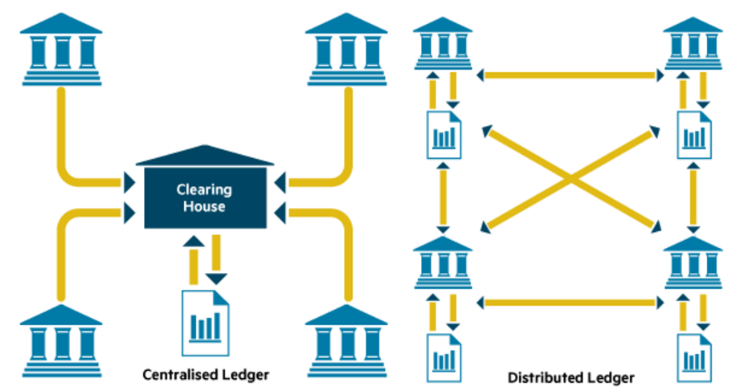
\includegraphics  [scale=0.35]{Images/ledger}
		\begin{centering}
			\caption{In a traditional market structure shown on the left, central clearing houses act as trusted intermediaries to facilitate the transfer of value and maintain a record of such transactions. Institutions keep their own records, but the single trusted source of information is the intermediary. If the market were to switch to blockchain based infrastructure, every institution would maintain its own copy of the ledger, the contents of which are visible to all other peers on the network and determined by a consensus protocol}
		\end{centering}
	\end{figure}
	\begin{tiny}
		Source: \href{https://beat.10ztalk.com/2017/10/09/what-is-a-blockchain-distributed-ledger-technology/}{https://beat.10ztalk.com/wp-content/uploads/2017/10/what-is-a-blockchain-distributed-ledger-technology.png}
	\end{tiny}
\end{frame}

% -----------------------------------------------------------------


\begin{frame}{What is a blockchain?}
	Although initially designed solely for Bitcoin network, blockchains can be used in any function that requires record keeping \\ \vspace{3mm}
	The technology has gained popularity in the financial services industry, because it enables multiple entities of conflicting interests to collaborate on maintaining a shared ledger of records and transact secrurely without the need for trust \\ \vspace{3mm}
	One of the core features of the technology is complete transparency
	\begin{itemize}
		\item Publicly accessible pseudonymous ownership records and complete transaction auditability are synonymous with the technology
		\item Blockchains therefore have the potential to provide unprecedented levels of transparency in the financial services industry
	\end{itemize}
\end{frame}

% -----------------------------------------------------------------

\begin{frame}
	\begin{figure}[]
		\centering
		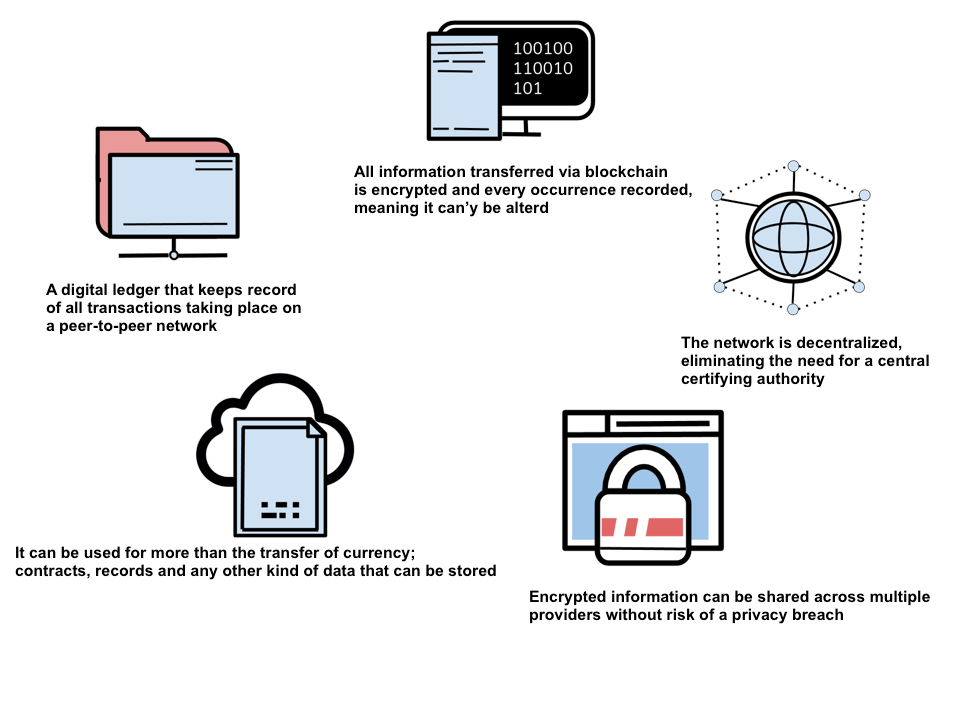
\includegraphics  [scale=0.3]{Images/block101}
	\end{figure}
\end{frame}

% -----------------------------------------------------------------

\begin{frame}
	\begin{figure}[]
		\centering
		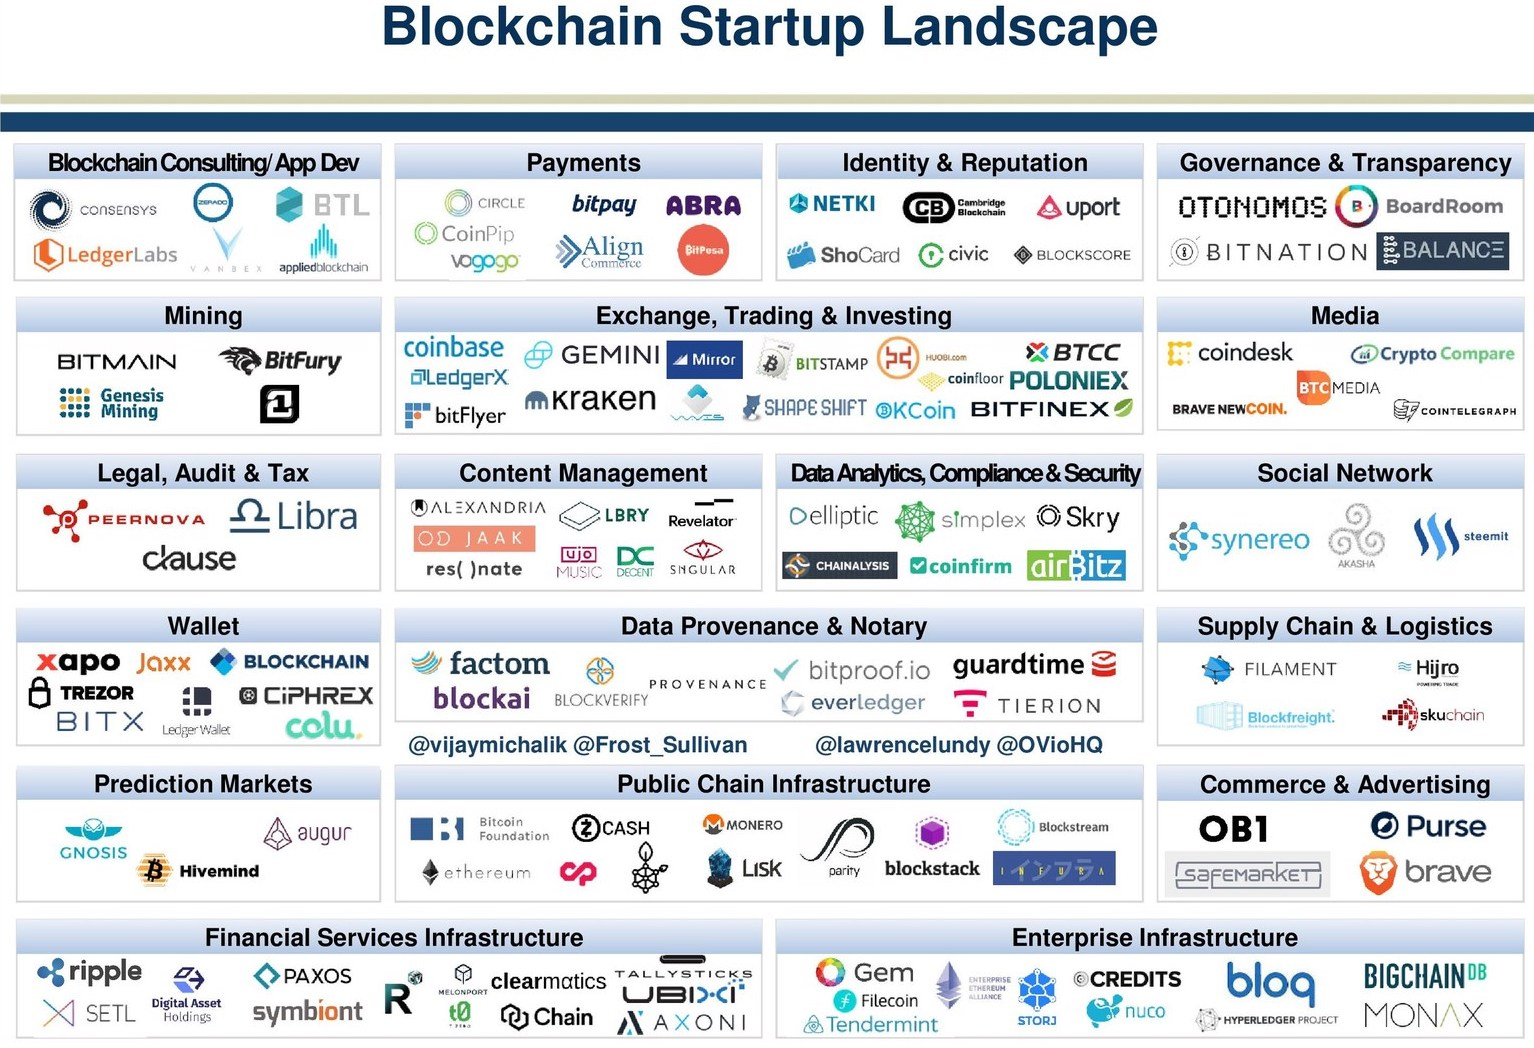
\includegraphics  [scale=0.2]{Images/blockchain-ecosystem}
	\end{figure}
	\begin{tiny}
		Source: \href{https://ww2.frost.com/news/press-releases/frost-sullivan-identifies-2017-global-blockchain-startup-map/}{https://ww2.frost.com/files/cache/a701d7ea2011161d4eaeed6364153683\_f16618.jpg}
	\end{tiny}
\end{frame}

% -----------------------------------------------------------------

\begin{frame}{Blockchain 101}
	\begin{small}
		\begin{itemize}
			\item Block - a dataset containing multiple records, and cryptographic elements to be appended onto the blockchain
			\item Blockchain - a data structure used to create a decentralized ledger
			\item Consensus - a process of agreement between distrusting nodes on a final state of data
			\item Cryptography - a set of techniques used for secure communication and storage of data
			\item Distributed system - a computing system where two or more nodes work together in a coordinated fashion to achieve a common outcome
			\item Distributed ledger - a append only list of records that is maintained using a consensus protocol
			\item Mining - the process of appending new information onto the distributed ledger, in the form of new blocks
			\item Peer to peer - communication protocol in which participating nodes have equal permissions and rights
			\item Proof of work - a consensus mechanism used to verify the validity of a block
		\end{itemize}
	\end{small}
\end{frame}

% -----------------------------------------------------------------

\begin{frame}
	\begin{figure}[]
		\centering
		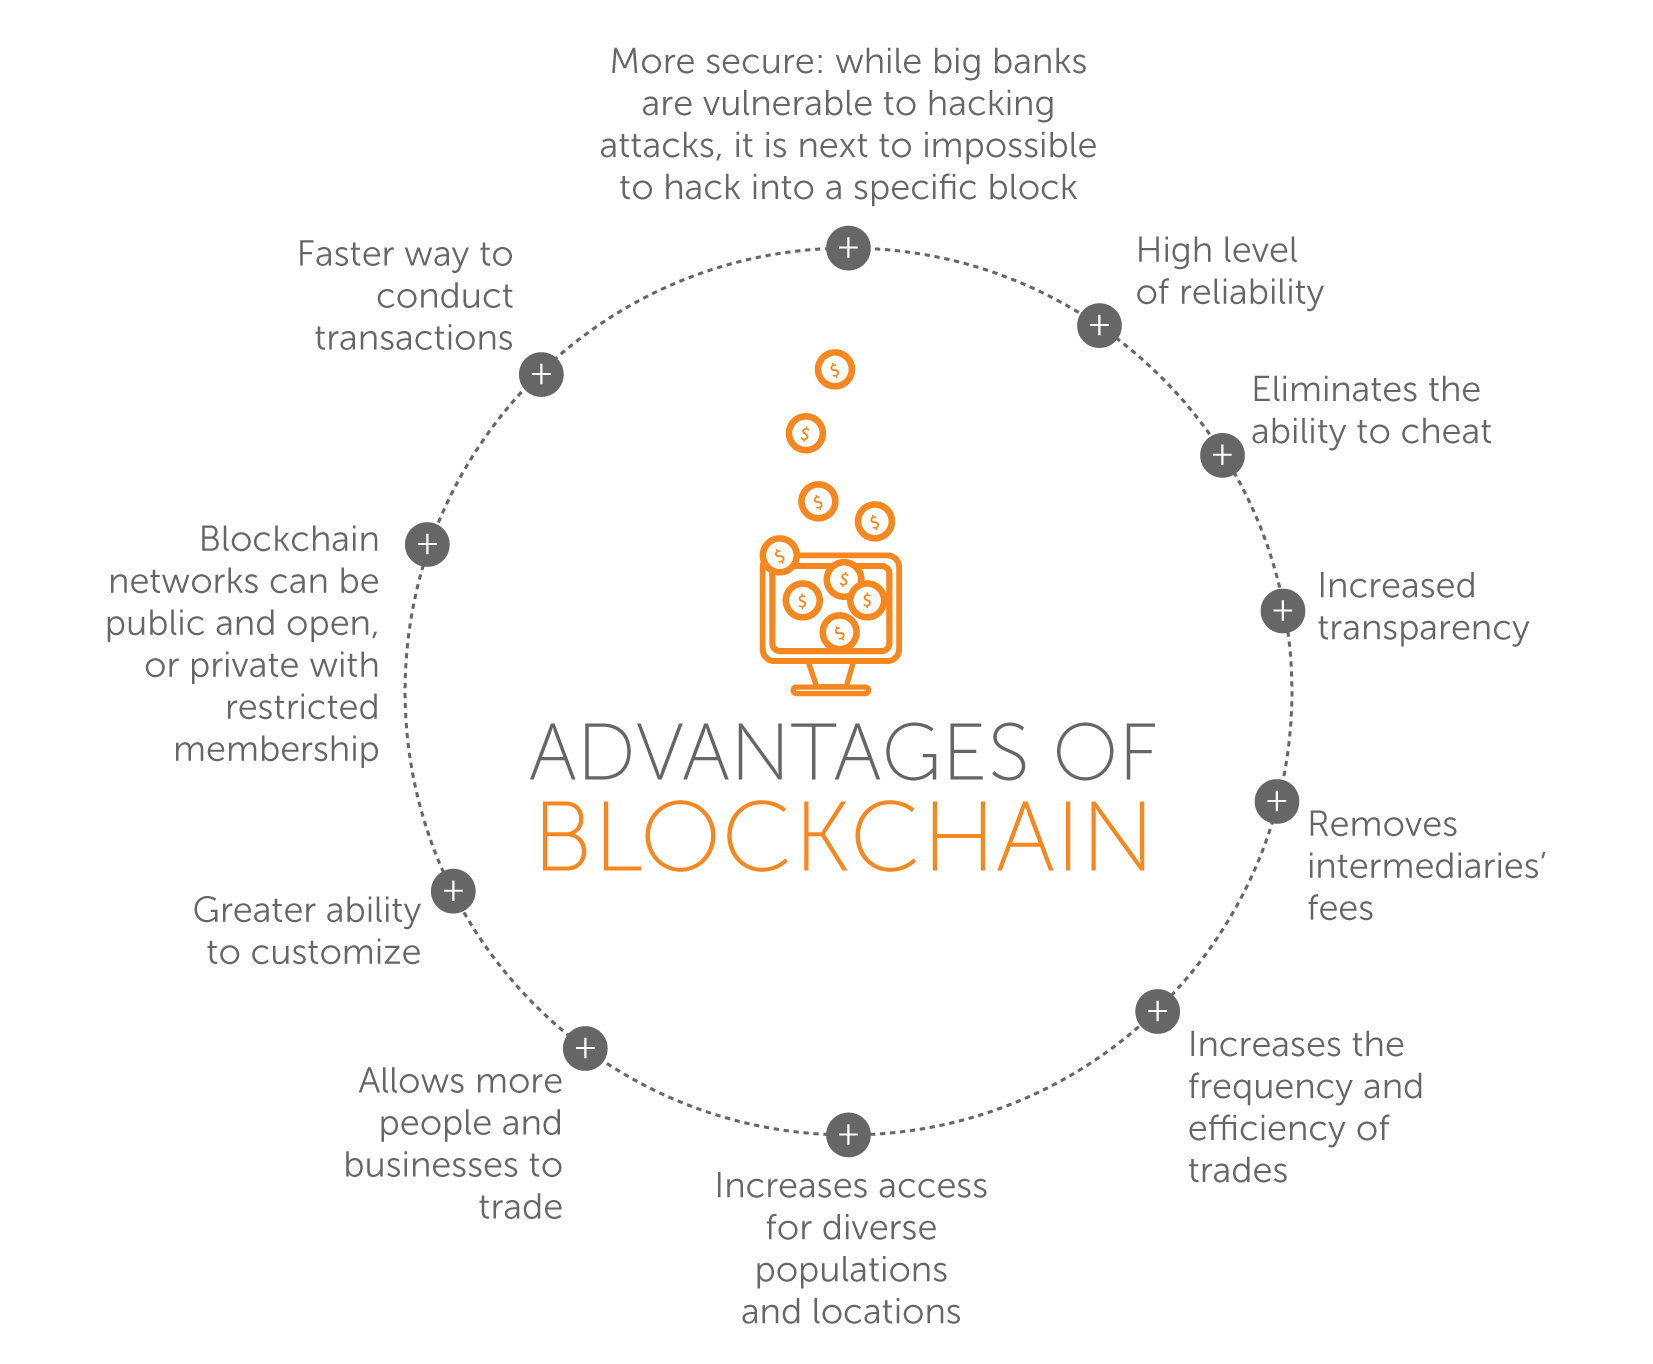
\includegraphics  [scale=0.15]{Images/advantages}
	\end{figure}
	\begin{tiny}
		Source: \href{http://www.arreverie.com/blogs/blockchain-technology-everything-need-know/advantages-of-bitcoin/}{http://www.arreverie.com/blogs/wp-content/uploads/2017/08/advantages-of-bitcoin-1024x845.jpg}
	\end{tiny}
\end{frame}

% -----------------------------------------------------------------

\begin{frame}{What is a blockchain?}
	A blockchain consists of 'blocks' linked together in a linear sequential chain\\ \vspace{3mm}
	Each block contains an encrypted identifier of the previous block (i.e. a hash), new transactions, a timestamp and a cryptographic nonce\\ \vspace{3mm}
	A nonce is an arbitrary 32-Bit number that may only be used once to verify the validity of the block that has been added to the chain
	\begin{figure}[]
		\centering
		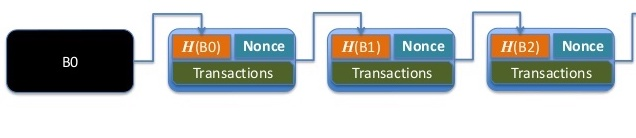
\includegraphics  [width=3.in]{Images/blockchain1}
	\end{figure}
	The size of the blocks determines the scalability of the network i.e. the number of transactions that are processed with each block that is added
	\begin{tiny}
		Source: \href{https://www.slideshare.net/DavidEvansUVa/the-blockchain}{https://image.slidesharecdn.com/class7-post-150921141838-lva1-app6892/95/the-blockchain-18-638.jpg?cb=1442845220}
	\end{tiny}
\end{frame}

% -----------------------------------------------------------------
\subsection{Cryptography}

\begin{frame}{Cryptography}
	\begin{itemize}
		\item Cryptography refers to a set of techniques used for secure communication and storage of data, such that it can be read and processed only by those for whom it is intended
		\item Blockchains effectively make use of cryptography in multiple different and complementary ways
		\item Its use includes and is not limited to
		\begin{itemize}
			\item The creation of pseudonymous identities
			\item Establishing a robust consensus mechanism
			\item Maintaining the immutability of the distributed ledger
			\item Providing secure communication that guarantees data integrity across the network
		\end{itemize}
	\end{itemize}
\end{frame}

	%introduce/summary of cryptography
	%https://en.bitcoin.it/wiki/How_bitcoin_works

% -----------------------------------------------------------------

\begin{frame}{Cryptography}
	\begin{figure}[]
		\centering
		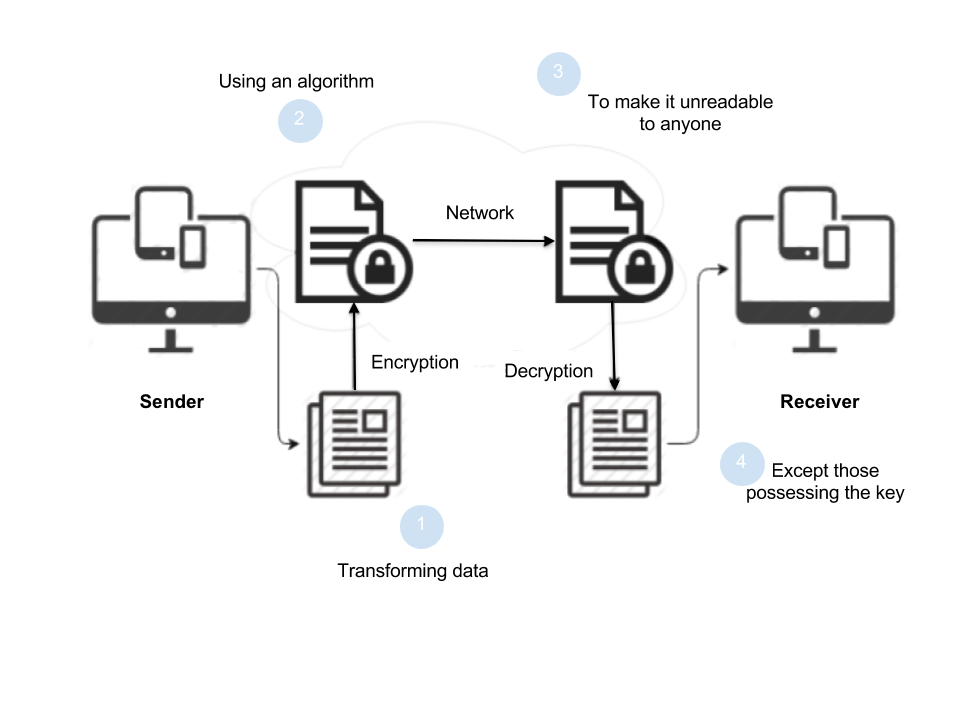
\includegraphics  [scale=0.3]{Images/cryptography}
		\begin{centering}
		\end{centering}
	\end{figure}
\end{frame}

% -----------------------------------------------------------------
\begin{frame}{Cryptography - Hash functions}
	Hash function
	\begin{itemize}
		\item A function that can be used to map data of arbitrary size to data of fixed size
		\item By comparing the output from execution of the algorithm to a known and expected hash value, one can determine the data's integrity
		\item Hash functions accelerate table or database lookup by detecting duplicated records in a large file
		\item A cryptographic hash function is a special class of hash function that is suitable for use in cryptography
	\end{itemize}
\end{frame}

% -----------------------------------------------------------------


\begin{frame}{Cryptography - Hash functions}
	The ideal cryptographic hash function has the following properties
	\begin{enumerate}
		\item[1] Collision resistance - output is sufficiently distinct hence it is infeasible to find two different messages with the same hash value
	\end{enumerate}
	\begin{figure}[]
		\centering
		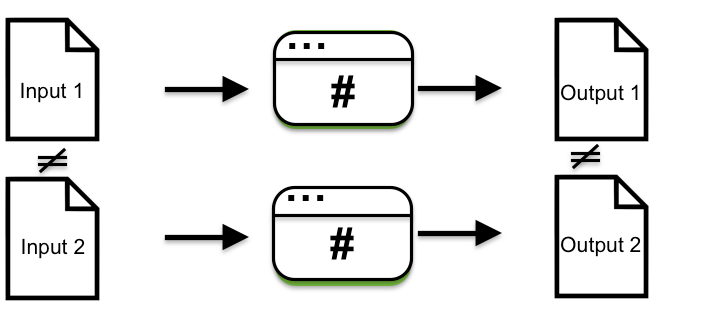
\includegraphics  [scale=0.3]{Images/hash1}
		\begin{centering}
		\end{centering}
	\end{figure}
\end{frame}

% -----------------------------------------------------------------

\begin{frame}{Cryptography - Hash functions}
	\begin{enumerate}
		\item[2] Deterministic - the same message always results in the same hash
	\end{enumerate}
	\begin{figure}[]
		\centering
		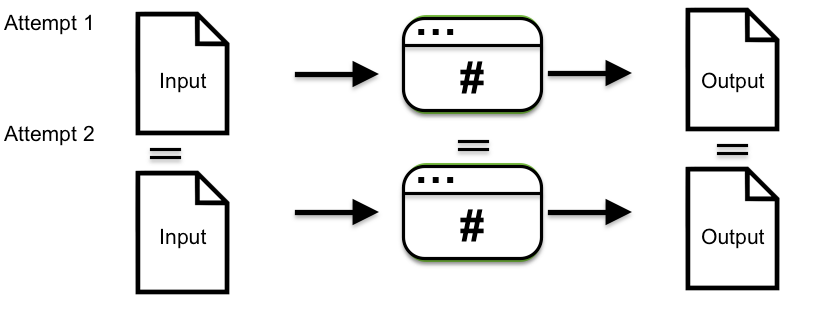
\includegraphics  [scale=0.3]{Images/hash2}
		\begin{centering}
		\end{centering}
	\end{figure}
\end{frame}

% -----------------------------------------------------------------

\begin{frame}{Cryptography - Hash functions}
	\begin{enumerate}
		\item[3] Concealing - it is infeasible to generate a message from its hash value except by trying all possible messages i.e. brute force search
	\end{enumerate}
	\begin{figure}[]
		\centering
		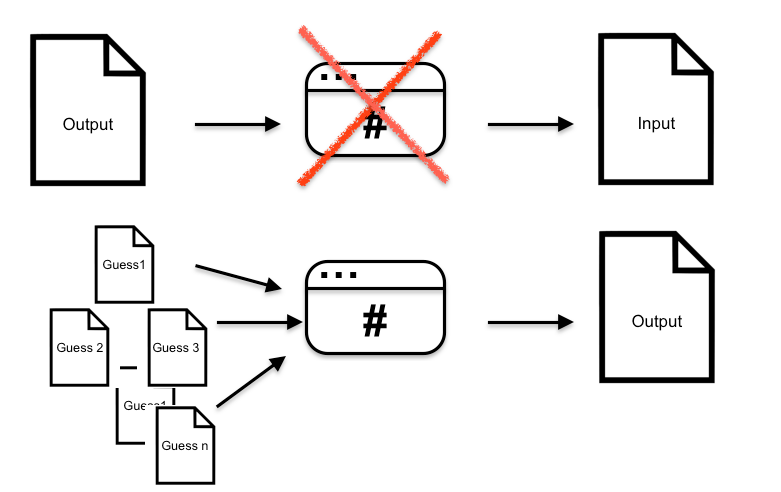
\includegraphics  [scale=0.3]{Images/hash3}
		\begin{centering}
		\end{centering}
	\end{figure}
\end{frame}

% -----------------------------------------------------------------

\begin{frame}{Cryptography - Hash functions}
	\begin{enumerate}
		\item[4] High avalanche effect - a small change to a message should change the hash value so extensively that the new hash value appears uncorrelated with the old hash value
	\end{enumerate}
	\begin{figure}[]
		\centering
		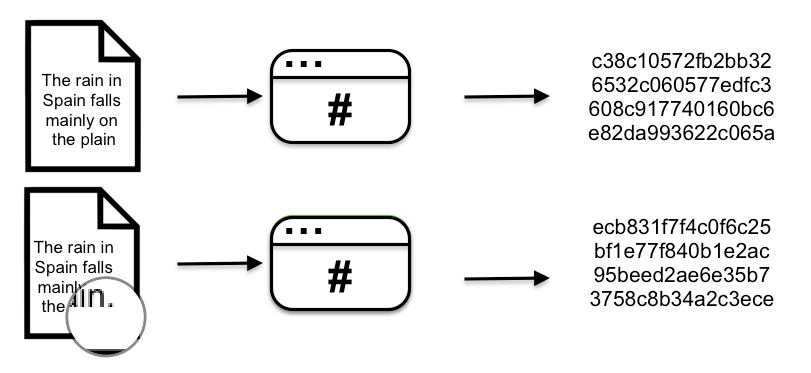
\includegraphics  [scale=0.3]{Images/hash4}
		\begin{centering}
		\end{centering}
	\end{figure}
\end{frame}

% -----------------------------------------------------------------

\begin{frame}{Cryptography - Hash functions}
	\begin{enumerate}
		\item[5] Quick to compute the hash value for any given message
	\end{enumerate}
	\begin{figure}[]
		\centering
		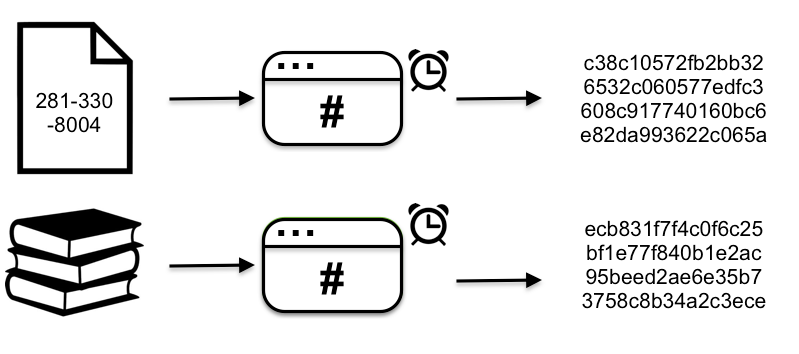
\includegraphics  [scale=0.3]{Images/hash5}
		\begin{centering}
		\end{centering}
	\end{figure}
\end{frame}

% -----------------------------------------------------------------


\begin{frame}{Cryptography - Hash functions}
	\begin{itemize}
		\item Collision resistance does not mean that no collisions exist; simply that they are hard to find
		\item The 'birthday paradox' can be used to understand why there exists an upper bound on collision resistance
		\begin{itemize}
			\item in a set of n randomly chosen people, the probability that some pair will have the same birthday increases with \textit{n}
			\item The probability reaches 100\% when the number of people reaches 367, since there are only 366 possible birthdays (99,9\% probability is reached with just 70 people)
			\item The same concept applies to hashes, given that they are of fixed length
			\item Theoretically, every hash function with more inputs than outputs will necessarily have collisions
		\end{itemize}
	\end{itemize}
\end{frame}


% -----------------------------------------------------------------

\begin{frame}{Birthday paradox}
	\begin{figure}[]
		\centering
		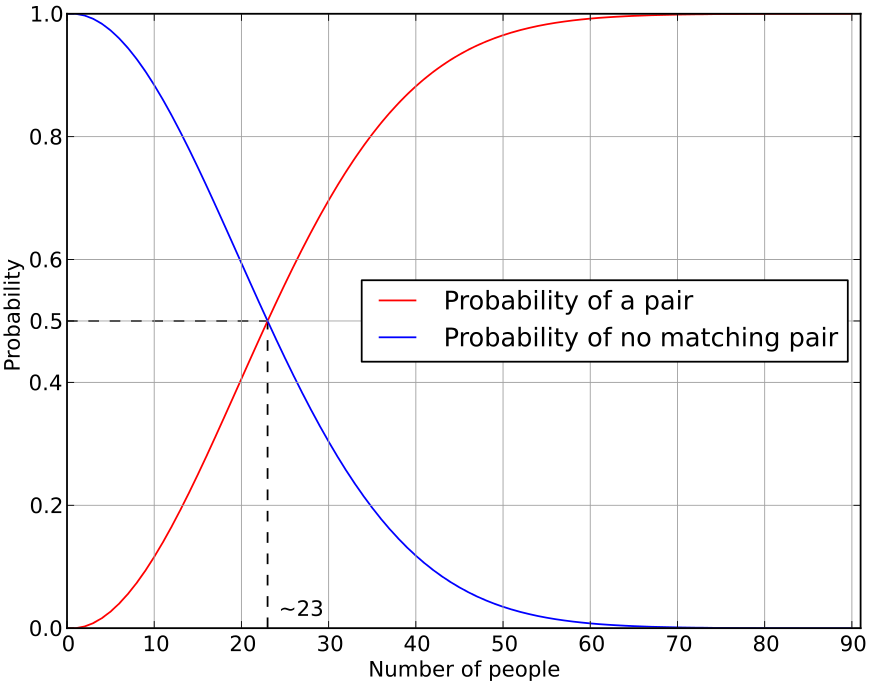
\includegraphics  [scale=0.2]{Images/paradox}
	\end{figure}
	\begin{tiny}
		Source: \href{https://en.wikipedia.org/wiki/File:Birthday_paradox_probability.svg}{https://en.wikipedia.org/wiki/File:Birthday\_paradox\_probability.svg}
	\end{tiny}
\end{frame}

% -----------------------------------------------------------------

\begin{frame}{Cryptography - Hash functions}
	\begin{itemize}
		\item Some hash functions that were previously thought to be collision resistant have been broken e.g. MD5 and SHA-1
		\item Currently there no hash function that is provably collision resistant, but there are hash functions for which a collision has not yet been found.
		\item NB. collision resistance is not sufficient to ensure the function is concealing
		\begin{itemize}
			\item Suppose the input has a known probability distribution that makes certain values more likely than others
			\item For practical purposes, one would need to know only the hashes associated with these inputs since the others are unlikely
			\item Hashes could therefore be pre-computed and looked up
		\end{itemize}
	\end{itemize}
\end{frame}
% -----------------------------------------------------------------

\begin{frame}{Cryptography - Hash functions}
	SHA256 hash
	\begin{itemize}
		\item Part of the SHA-2 set of cryptographic hash functions designed by the United States NSA
		\item Several cryptocurrencies use SHA-256 for verifying transactions and calculating proof-of-work or proof-of-stake
		\item It is also used in the creation of node addresses in order to improve security and privacy
	\end{itemize}
\end{frame}

% -----------------------------------------------------------------

\begin{frame}{Cryptography - Binary trees}
	Blockchains use binary trees to store data \\ \vspace{3mm}
	This is a tree data structure in which each node has at most two children, which are referred to as the left child and the right child \\ \vspace{3mm}
	This data structure is often preferred as it enables efficient searching of large data sets through the use of the principle of binary search \\ \vspace{3mm}
	When searching for a specific point in the tree, lookups and other operations will traverse the tree from root to leaf, at each point deciding to continue searching in the left or right subtrees \\ \vspace{3mm}
	This significantly reduces search time, as on average this allows the operations to skip half the tree
\end{frame}

% -----------------------------------------------------------------

\begin{frame}{Cryptography - Binary trees}
	\begin{figure}[]
		\centering
		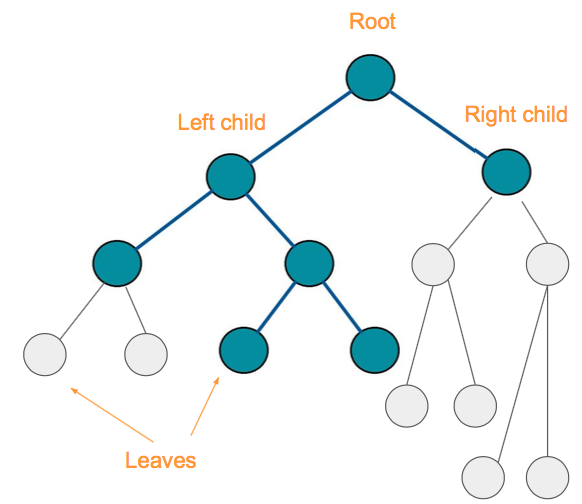
\includegraphics  [scale=0.3]{Images/binary}
		\caption{A binary tree}
	\end{figure}
\end{frame}

% -----------------------------------------------------------------

\begin{frame}{Cryptography - Merkle trees}
	Merkle tree roots
	\begin{itemize}
		\item Transactions are stored in a block header in the form of a Merkle tree root
		\item This is a type of binary tree in which every non-leaf is constructed from the hashes of its child nodes, with the transaction IDs as the leaf nodes
		\item This allows for efficient and secure verification of the contents of large data structures
	\end{itemize}
\end{frame}

% -----------------------------------------------------------------

\begin{frame}{Cryptography - Merkle trees}
	The Merkle root is cryptographic proof of which transactions are in the block, and which order they are in.
	\begin{figure}[]
		\centering
		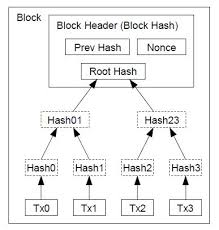
\includegraphics  [scale=0.5]{Images/images}
	\end{figure}
	\begin{tiny}
		Source: \href{https://bitcoin.org/bitcoin.pdf}{https://bitcoin.org/bitcoin.pdf}
	\end{tiny}
\end{frame}

% -----------------------------------------------------------------

\begin{frame}{Simple payment verification}
	\begin{itemize}
		\begin{small}
			\item It is possible to conform the existence of a transaction in a block without having to download the entire blockchain
			\item By keeping copies of only the block headers, transactions can be verified using Merkle trees
			\item A user only needs to obtain the Merkle branch linking the transaction to the Merkle tree root
			\item Proof of inclusion is obtained by reconstructing the root using the transaction hash and non leaf nodes of the pruned Merkle branch
		\end{small}
	\end{itemize}
	\begin{figure}[]
		\centering
		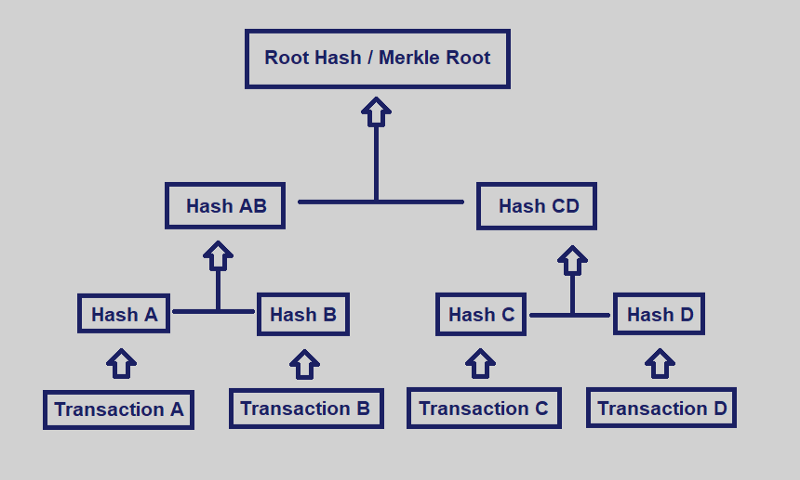
\includegraphics  [scale=0.3]{Images/spv}
	\end{figure}
	\begin{tiny}
		Source: \href{https://bitcoin.org/bitcoin.pdf}{https://bitcoin.org/bitcoin.pdf}
	\end{tiny}
\end{frame}

% -----------------------------------------------------------------

\begin{frame}{Cryptography}
	\begin{figure}[]
		\centering
		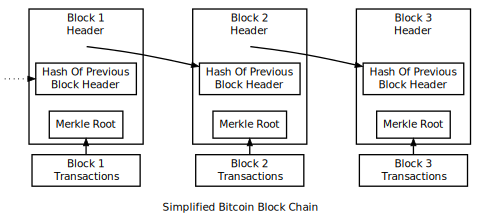
\includegraphics  [width=4.in]{Images/blockchain}
	\end{figure}
	\begin{tiny}
		Source: \href{https://bitcoin.org/en/developer-guide}{https://bitcoin.org/img/dev/en-blockchain-overview.svg}
	\end{tiny}
\end{frame}

% -----------------------------------------------------------------

\begin{frame}{Cryptography}
	\begin{scriptsize}
		Bitcoin block information
	\end{scriptsize}
	\begin{figure}[]
		\centering
		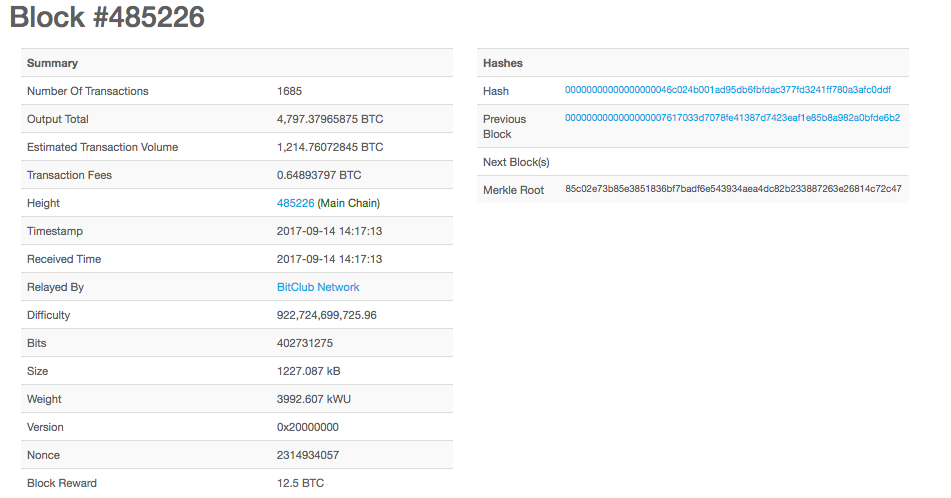
\includegraphics  [width=4.in]{Images/block}
	\end{figure}
	\begin{tiny}
		Source: blockchain.info
	\end{tiny}
\end{frame}

% -----------------------------------------------------------------

\subsection{Public key cryptography}

\begin{frame}
	\begin{figure}[]
		\centering
		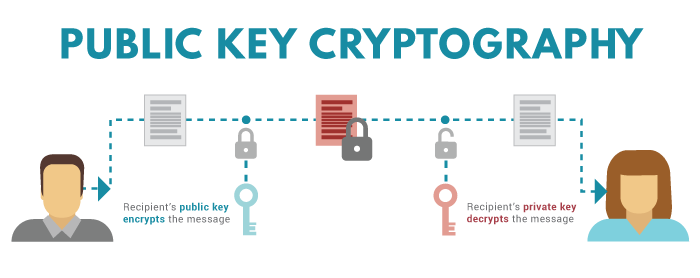
\includegraphics  [width=4.in]{Images/publickey1}
	\end{figure}
	\begin{tiny}
		Source: \href{https://eng.paxos.com/blockchain-separating-hype-from-substance-part-2}{https://eng.paxos.com/hs-fs/hubfs/\_02\_Paxos\_Engineering/Public-Key-Cryptography-1.png?t=1513284613258\&width=1024\&name=Public-Key-Cryptography-1.png}
	\end{tiny}
\end{frame}

	%https://eng.paxos.com/blockchain-separating-hype-from-substance-part-2

% -----------------------------------------------------------------

\begin{frame}{Public key cryptography}
	\begin{itemize}
		\item Traditional blockchain implementations make use of public key/asymmetric cryptography
		\item This is a form of cryptography where there are two keys called a private key and a public key
		\item The public key is derived from an algorithmic transformation the private key
		\item Hashing the public key give the blockchain address
	\end{itemize}
	\begin{figure}[]
		\centering
		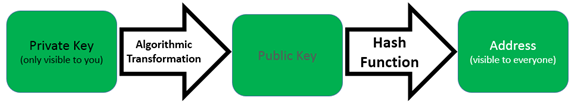
\includegraphics  [scale=0.3]{Images/keys}
	\end{figure}
\end{frame}



% -----------------------------------------------------------------

\begin{frame}{Public key cryptography}
	Encryption and signing
	\begin{itemize}
		\item Data encrypted with the private key an only be decrypted with the corresponding public key and vise versa
		\begin{itemize}
			\item A message can be signed by encrypting its hash with the private key; any one with the corresponding public key can decrypt it, but only you could have encrypted it
			\item If a message is encrypted using the public key, only the corresponding private key can decrypt it
		\end{itemize}
		\item A message can be signed with the sender's private key and then encrypted with the recipient's public key
		\item The integrity of a blockchain is dependent on private keys remaining hidden
	\end{itemize}
\end{frame}



% -----------------------------------------------------------------

\begin{frame}{Public key cryptography}
	\begin{itemize}
		\item Traditional blockchain implementations make use of the Elliptic Curve Digital Signature Algorithm (ECDSA) to sign transactions and generate key pairs
		\item Each coin is associated with its current owner's public ECDSA key
		\item Transactions are fundamentally messages containing the new owner's public key, the amount of the item being transferred and signed by the sender's private key
		\item The signature is used to verify the authenticity of the message
	\end{itemize}
\end{frame}

% -----------------------------------------------------------------

\begin{frame}{Public key cryptography}
	\begin{columns}
	    \column{0.5\textwidth}
		\begin{figure}[]
			\centering
			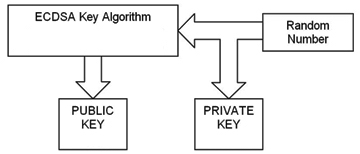
\includegraphics  [scale=0.4]{Images/ECDSA3}
			\caption{Key pair generation}
		\end{figure}
		\column{0.5\textwidth}
		\begin{itemize}
			\item A random number generator is used to produce a value that becomes the private key
			\item Next the public key is computed according to the ECDSA key pair algorithm
		\end{itemize}
	\end{columns}
	\begin{tiny}
		Source: \href{https://eng.paxos.com/blockchain-separating-hype-from-substance-part-2}{https://m.eet.com/media/1203927/Maxim\%20ECDSA\%20Figure\%202.jpg}
	\end{tiny}
\end{frame}


% -----------------------------------------------------------------

\begin{frame}{Public key cryptography}
	\begin{columns}
		\column{0.5\textwidth}
		\begin{figure}[]
			\centering
			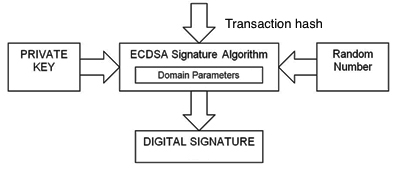
\includegraphics  [scale=0.4]{Images/ECDSA1}
			\caption{Signature computation process}
		\end{figure}
		\column{0.5\textwidth}
		\begin{itemize}
			\item A digital signature allows the recipient of a message to verify its authenticity using the senders public key
			\item To produce a signature, the message first has to be converted to a fixed length message sing a secure hash algorithm
			\item To produce the signature the ECDSA signature algorithm takes in as input the message has, the sender's private key and a random number
		\end{itemize}
	\end{columns}
	\begin{tiny}
		Source: \href{https://eng.paxos.com/blockchain-separating-hype-from-substance-part-2}{https://m.eet.com/media/1203929/Maxim\%20ECDSA\%20Figure\%203.jpg}
	\end{tiny}
\end{frame}

	%https://www.embedded.com/design/safety-and-security/4427811/Using-the-Elliptic-Curve-Digital-Signature-Algorithm-effectively


% -----------------------------------------------------------------

\begin{frame}{Public key cryptography}
	\begin{columns}
		\column{0.5\textwidth}
		\begin{figure}[]
			\centering
			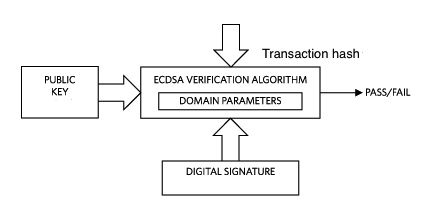
\includegraphics  [scale=0.4]{Images/ECDSA2}
			\caption{Signature verification process}
		\end{figure}
		\column{0.5\textwidth}
		\begin{itemize}
			\item Using the same secure hash algorithm as the signature algorithm, the message hash is computed
			\item The verification algorithm takes in as input the digital signature, the sender's public key and the hashed message
		\end{itemize}
	\end{columns}
	\begin{tiny}
		Source: \href{https://eng.paxos.com/blockchain-separating-hype-from-substance-part-2}{https://m.eet.com/media/1203932/Maxim\%20ECDSA\%20Figure\%204.jpg}
	\end{tiny}
\end{frame}


% -----------------------------------------------------------------

% \begin{frame}{How does it work?}
% Public key and private keys
% \begin{itemize}
% \item Transactions on a blockchain are sent to a hashed version of the 'public key'
% \begin{itemize}
% \item This is a public address that is visible to every node on the blockchain
% \item The public key is derived from an algorithmic transormation of a 'private key'
% \end{itemize}

% \begin{figure}[]
% \centering
% 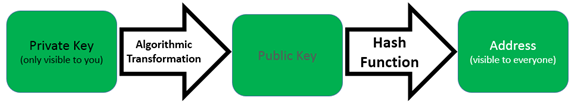
\includegraphics  [width=3.in]{Images/keys}
% \end{figure}
% %\item Every public key has a corresponding private key
% %\begin{itemize}
% %\item This private key is what controls access to the assets held by the public key
% %\item In order for a transaction to be valid, it must be signed by the private key
% %\item This signature is in the form of a hash of the private key
% %\end{itemize}
% \end{itemize}
% \end{frame}

% -----------------------------------------------------------------


% \begin{frame}{How does it work?}
% In order for a transaction to be valid, it must be signed by the private key
% \begin{itemize}
% \item The private key is also used to generate a signature that is included in a transaction, to confirm that it has come from the rightful user
% \end{itemize}
% The integrity of a blockchain is dependent on private keys remaining hidden
% \begin{itemize}
% \item Anyone with the private key can use it to transact with the respective public address
% \end{itemize}
% \end{frame}

% -----------------------------------------------------------------

\begin{frame}{Failure of public key cryptography - Mt Gox hack}
	Mt. Gox was a Bitcoin exchange based Tokyo that collapsed in 2014 after it got hacked ; at its peak, Mt Gox handled 70\% of bitcoin transactions worldwide \\ \vspace{3mm}
	Hackers gained access to private keys held by the exchange on behalf of its customers, after which they stole over \$450million from the exchanges' 'hot wallet'
	\begin{itemize}
		\item A hot wallet is a cryptocurrency wallet that is connected to the internet
	\end{itemize}
	This marked the second major hack that the company faced
	\begin{itemize}
		\item Previously in June 2011 hackers got away with the equivalent of \$8.75million
		\item Allegedly hackers had been skimming money from the company for years
	\end{itemize}
	Inadequate governance contributed to the exchanges' security flaws
%https://www.wired.com/2014/03/bitcoin-exchange/
\end{frame}

% -----------------------------------------------------------------

\subsection{Peer to peer networks}

\begin{frame}{Peer to peer networks}
	\begin{itemize}
		\item In peer to peer networks, peers are equally privileged, equipotent participants
		\item Peers are both suppliers and consumers of resources as there are no client-server relationships
		\item All nodes have the ability to directly communicate
		\item Blockchains are designed to be peer to peer networks, every node is allowed to send new transactions, verify transactions, and create new blocks
	\end{itemize}
\end{frame}
% -----------------------------------------------------------------

\begin{frame}{Peer to peer networks}
	\begin{figure}[]
		\centering
		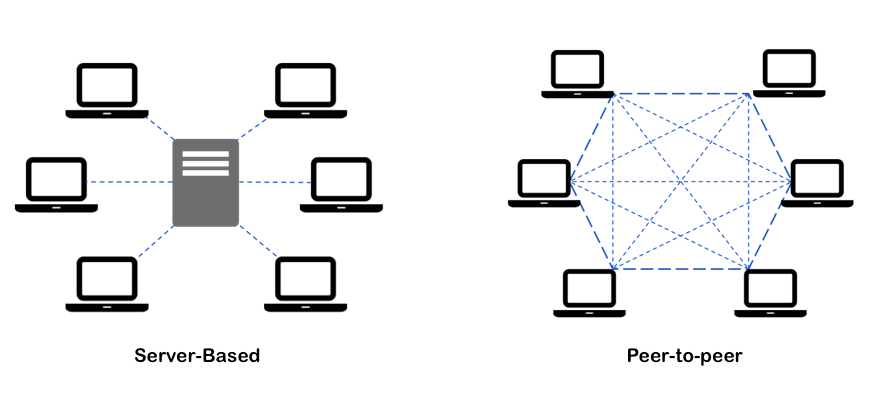
\includegraphics  [scale=0.3]{Images/p2p}
	\end{figure}
\end{frame}

% -----------------------------------------------------------------

\begin{frame}{Peer discovery}
	\begin{itemize}
		\item Peer to peer networks do not impose a particular structure on how communication occurs
		\item A node does not need to connect to every node in the network in order to broadcast and listen to new transactions/blocks
		\item By connecting to a few neighbors, which in turn connect to their neighbors, the whole network remains connected
		\item The way in which peers locate each other will vary by blockchain design
		\item One way is for the client to use a list of nodes from a previous connection to the network
	\end{itemize}
\end{frame}

% -----------------------------------------------------------------

\begin{frame}
	\begin{figure}[]
		\centering
		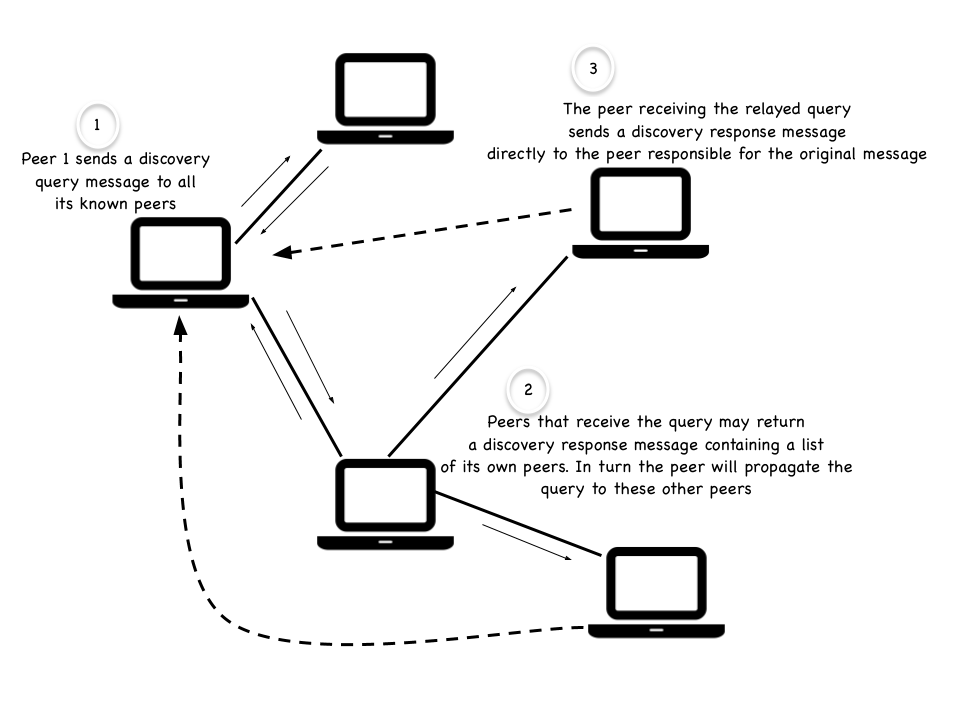
\includegraphics  [scale=0.3]{Images/p2pdisc}
	\end{figure}
\end{frame}

% -----------------------------------------------------------------

\begin{frame}{Peer discovery}
	\begin{itemize}
		\item Another way is through the use of bootnodes i.e. a node hardcoded in the node discovery protocol, that maintains a list of all nodes that have recently connected to it.
		\item When a node, connects to the network, it will automatically connect to the bootnode, which will then share the list of peers to which it can connect
		\item Nodes can generally be split into 3 categories, each with multiple variations: Full nodes, Pruned full nodes and Simple payment verification nodes
	\end{itemize}
\end{frame}

% -----------------------------------------------------------------

\begin{frame}{Node design}
	\begin{enumerate}
		\item Full nodes
			\begin{itemize}
				\item Download every block and transaction and check them against the blockchain's core consensus rules
				\item Require significant bandwidth to allow efficient propagation of data and substantial RAM to process a certain number of transactions per second
				\item There are two types of full nodes. Regular nodes only keep copies of the blockchain, and mining nodes build the blockchain
			\end{itemize}
		\item Pruned full nodes
			\begin{itemize}
				\item Only store the most recent blocks, but are still able to verify all transactions that occur on the blockchain
			\end{itemize}
		\item Simple payment verification (SPV) nodes
			\begin{itemize}
				\item Are only able to use Merkle trees to confirm a transactions existence in a block through the reproduction of hashes
				\item Validate the existence of transactions without being subjected to the load of operating a full node
				\item store only block headers and not contents
			\end{itemize}
	\end{enumerate}
\end{frame}

% -----------------------------------------------------------------

\begin{frame}{Node design}
	\begin{figure}[]
		\centering
		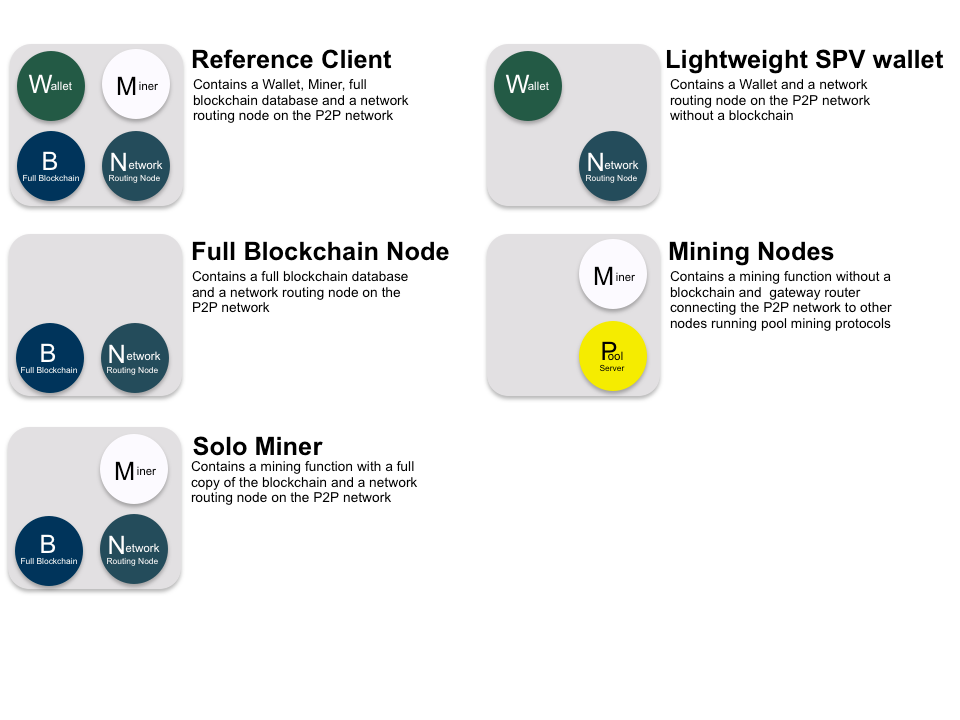
\includegraphics  [scale=0.35]{Images/nodes}
	\end{figure}
\end{frame}

% -----------------------------------------------------------------

\subsection{Types of blockchains}

\begin{frame}{Types of blockchains}
	\begin{itemize}
		\item Blockchains were initially intended to be public and completely transparent in all aspects
		\item However, efforts by are continually being made by institutions to leverage this database structure in examples with varying levels of transparency, anonymity and decentralization
		\item We can therefore divide blockchains into multiple types with distinct but sometimes partly overlapping attributes
	\end{itemize}
\end{frame}

% -----------------------------------------------------------------

\begin{frame}{Public blockchains}
	\begin{itemize}
		\item As the name suggests, these blockchains are open to the public and anyone can participate as a node in the decision making process
		\item These blockchains are also known as permission-less ledgers
		\item All users maintain a copy of the ledger on their local nodes, and use a distributed consensus mechanism in order to reach a decision about the eventual state of the ledger
		\item The majority of cryptocurrencies fall under this category
	\end{itemize}
\end{frame}

% -----------------------------------------------------------------

\begin{frame}{Private blockchains}
	\begin{itemize}
		\item Open only to a consortium or group of individuals or organizations that has decided to share the ledger among themselves
		\item These do away with pseudonymous identities, hence all participating nodes are known.
		\item Proprietary blockchains are a subset of private blockchains that deviate from the fundamental idea of decentralization of the technology
		\item These are typically used within an organizations, hence many traditional features become superfluous due to the absence of conflicting interests
	\end{itemize}
\end{frame}

% -----------------------------------------------------------------

\begin{frame}{Permissioned ledgers}
	\begin{itemize}
		\item A class of blockchains that also does away with pseudonymous identities and access is controlled by a group of nodes
		\item These do not need to use a distributed consensus mechanism, instead an agreement protocol can be used to maintain a shared version of truth about the state of the records
		\item Neither is there a requirement for permissioned blockchains to be private as they can be public blockchains but with regulated access control
	\end{itemize}
\end{frame}

% -----------------------------------------------------------------

\begin{frame}
	\begin{figure}[]
		\centering
		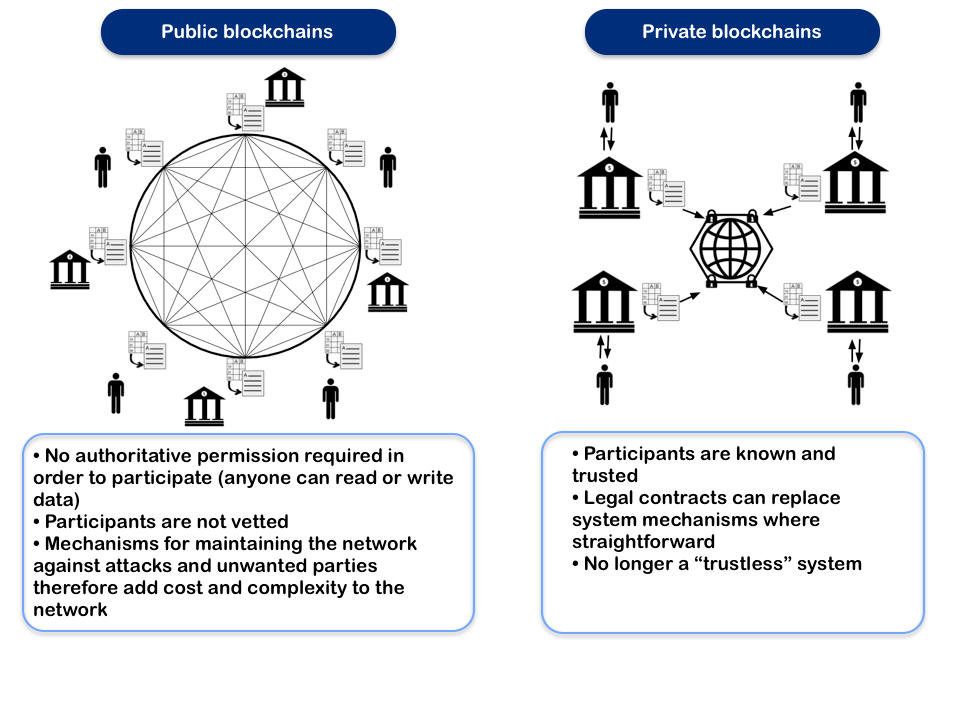
\includegraphics  [scale=0.3]{Images/pvt}
	\end{figure}
\end{frame}

% -----------------------------------------------------------------

\begin{frame}{Genesis block}
	\begin{itemize}
		\item This is the very first block of a blockchain and it is assigned to block number zero
		\item It is a special block in that it does not reference a previous block, neither does it contain any transactions
		\item Two nodes in a network will only pair with each other and synchronize if they have identical genesis blocks
		\item This block is typically hardcoded into the clients used to access the network
	\end{itemize}
\end{frame}

% -----------------------------------------------------------------

\begin{frame}{Bitcoin genesis}
	\begin{figure}[]
		\centering
		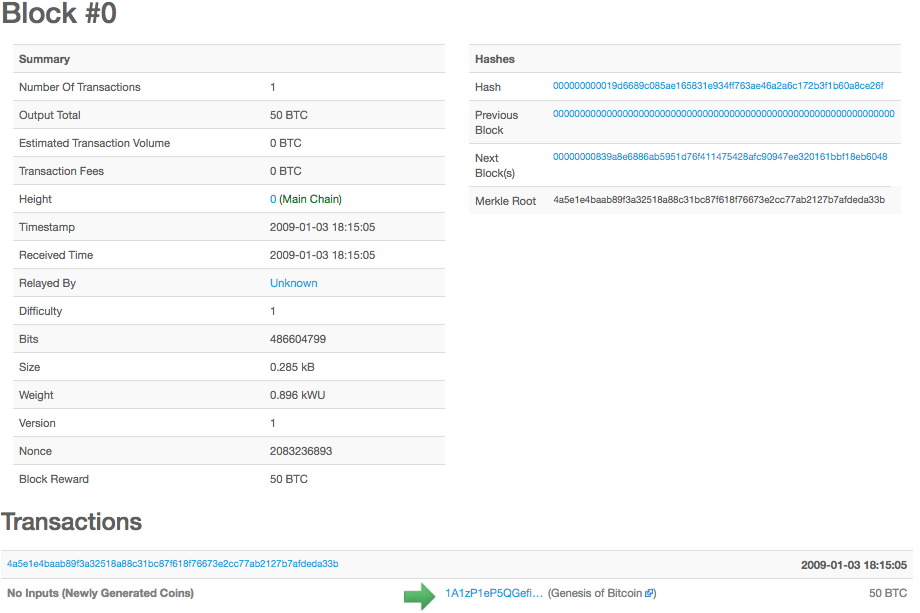
\includegraphics  [width=90mm]{Images/genesis}
	\end{figure}
\end{frame}

% -----------------------------------------------------------------

\subsection{Transactions}

\begin{frame}{Bitcoin transaction structure}
	\begin{itemize}
		\item Because bitcoins exist only as records of transactions, you can end up with many different transactions tied to a particular address
		\item These are not automatically combined but instead sit there as different transaction records
		\item Although it would be possible to handle coins individually, it would be inefficient to make a separate transaction for every cent in a transfer
		\item To allow value to be split and combined, transactions contain multiple inputs and outputs
		\begin{itemize}
			\item Input - A reference to an output from a previous transaction i.e. a record of the value and address used to send the coins being sent in the current transaction. The value being sent in a transaction can be the combination of the value received in multiple previous transactions
			\item Output - Contain instructions for the sending of bitcoins i.e. recipient address and value. Each output then waits as an Unspent Transaction Output (UTXO) until a later input spends it
		\end{itemize}
	\end{itemize}
\end{frame}

% -----------------------------------------------------------------

\begin{frame}{Bitcoin transaction structure}
	\begin{itemize}
		\item Every transaction must refer to one or more previously mined transactions, therefore the entire combined input value needs to be spent in an output
		\item If the input is worth 50 BTC but you only want to send 25 BTC, two outputs worth 25 BTC will be created: one to the destination, and one back to you (i.e. change)
		\item Any input bitcoins not redeemed in an output is considered a transaction fee, hence whoever generates the block will get it
	\end{itemize}
\end{frame}

% -----------------------------------------------------------------

\begin{frame}{Bitcoin transaction structure}
	\begin{itemize}
		\item A transaction at a high level contains the following
		\begin{itemize}
			\item Metadata - This part contains values such as the size of the transaction and its hash
			\item Inputs -  Has three fields. Previous tx is a hash of a previous transaction, Index is the specific output in the referenced transaction and ScriptSig is the first half of a script that contains a signature and a public key
			\item Outputs - Outputs have only two fields Value and ScriptPubKey. The first field contains the value being sent and the second is a locking script that contains the conditions that need to be met in order for the output to be spent.
		\end{itemize}
	\end{itemize}
\end{frame}

	% https://en.bitcoin.it/wiki/Transaction
	% https://www.bitcoin.com/info/how-bitcoin-transactions-work
	% http://davidederosa.com/basic-blockchain-programming/inside-transactions/
	% https://bitcoin.stackexchange.com/questions/52550/bitcoin-transaction-structure
	% https://bitcoin.org/bitcoin.pdf

% -----------------------------------------------------------------

\begin{frame}{Bitcoin transaction structure}
	\begin{figure}[]
		\centering
		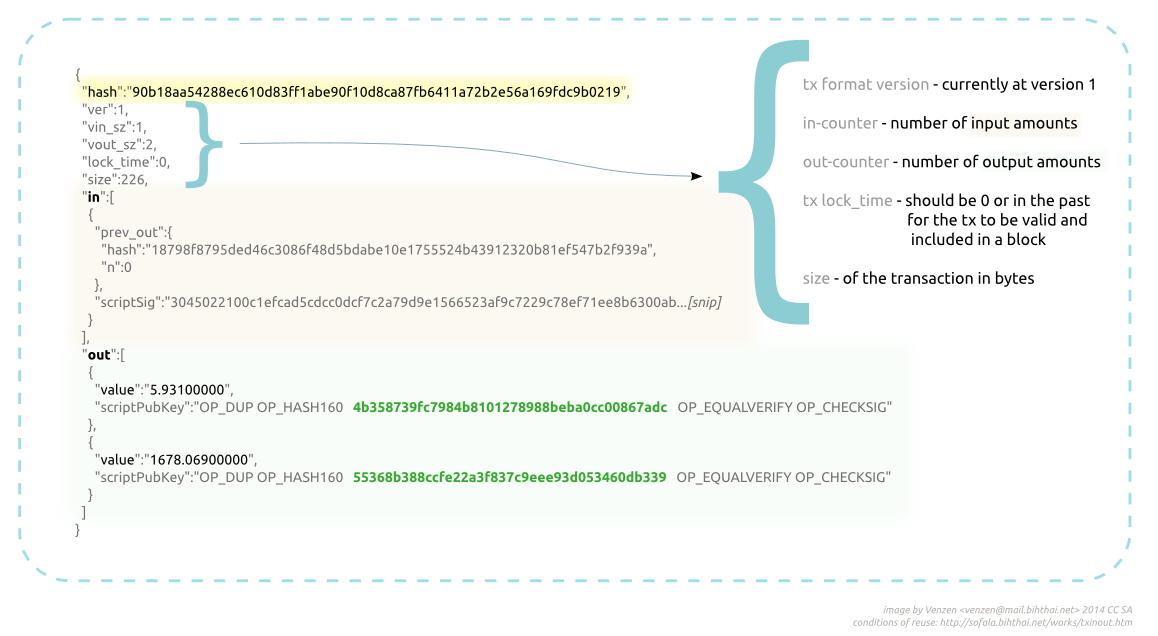
\includegraphics  [scale=0.25]{Images/tx}
	\end{figure}
	\begin{tiny}
		Source: \href{https://www.ccn.com/bitcoin-transaction-really-works/}{https://248qms3nhmvl15d4ne1i4pxl-wpengine.netdna-ssl.com/wp-content/uploads/2014/07/Bitcoin\_tx\_example.png}
	\end{tiny}
\end{frame}

% -----------------------------------------------------------------

\begin{frame}{Bitcoin transaction structure}
	\begin{itemize}
		\item Because each transaction spends value previously received in one or more earlier transactions, transactions are also chained together
		\item All transactions included in the blockchain are categorized as either UTXOs or spent transaction outputs.
		\item For a payment to be valid, it must only use UTXOs as inputs, and if the value of outputs exceeds that of inputs, the transaction will be rejected
		\item Outputs are tied to transaction identifiers (TXIDs), which are the hashes of signed transactions
	\end{itemize}
\end{frame}

% -----------------------------------------------------------------

\begin{frame}{Bitcoin transaction structure}
	\begin{figure}[]
		\centering
		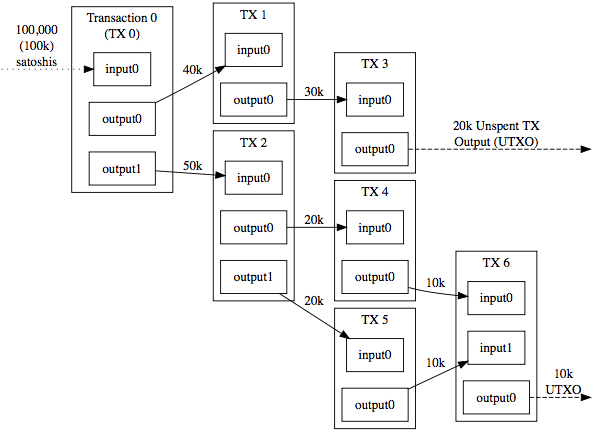
\includegraphics  [scale=0.4]{Images/tx-chain}
		\caption{Transaction chain with a fee of 10k satoshi}
	\end{figure}
	\begin{tiny}
		Source: \href{https://blog-archive.bitgo.com/the-challenges-of-block-chain-indexing/}{https://blog-archive.bitgo.com/content/images/2015/05/txchains.png}
	\end{tiny}
\end{frame}

% -----------------------------------------------------------------

\begin{frame}{Blockchain transactions}
	\begin{itemize}
		\item Account balances aren't explicitly maintained, but are implied by transactions into the accounts
		\item When validating blocks and transactions, nodes are offered transaction fees as a participation incentive
		\item Because, the larger the transaction data size, the longer and more energy it will take to validate the data
	\end{itemize}
\end{frame}

% -----------------------------------------------------------------

\begin{frame}{Choosing which output to spend}
	\begin{figure}[]
		\centering
		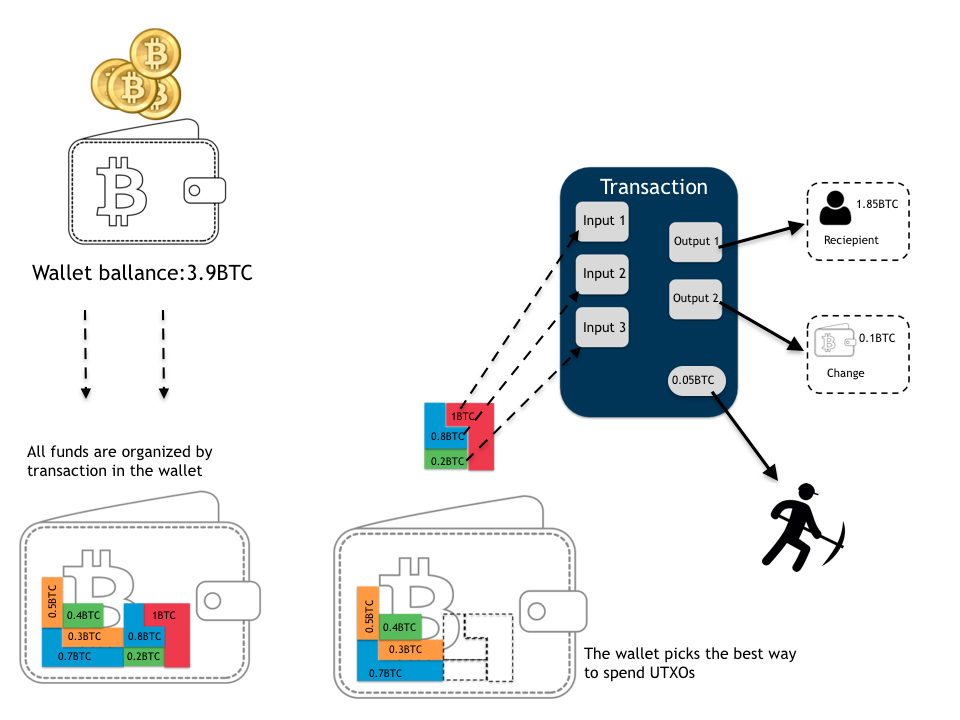
\includegraphics  [scale=0.3]{Images/spend}
	\end{figure}
\end{frame}

% -----------------------------------------------------------------

\begin{frame}{Transaction fees}
	\begin{itemize}
		\item The sender is required to pay the full transaction fee on top of the amount being transfered
		\item Considering that block size is limited, transaction fees can be seen as the cost of purchasing a portion of block space for a transaction, an incentive to mining nodes to include a particular transaction in the next block
		\item This fee is therefore determined by the size of the transaction data and is independent of the value being transferred
		\item The price of this block space is completely driven by supply and demand. When demand is high, fees are higher
	\end{itemize}
\end{frame}

% -----------------------------------------------------------------

\begin{frame}{Transaction fees}
	\begin{itemize}
		\item Typically, users will pay a fee imposed by cryptocurrency wallet providers that use predictive algorithms to determine the required fee per byte of transaction data
		\item However, transaction fees are voluntary on the part of the person making the transaction. A user may opt to pay lower fees or no fees at all, although, this will lower the priority of the transaction and increase confirmation time
		\item Transactions that generate higher fees will always be confirmed faster, as participating mining nodes set out maximize their utility
	\end{itemize}
\end{frame}

% -----------------------------------------------------------------

\begin{frame}
	\begin{scriptsize}
	\end{scriptsize}
	\begin{figure}[]
		\centering
		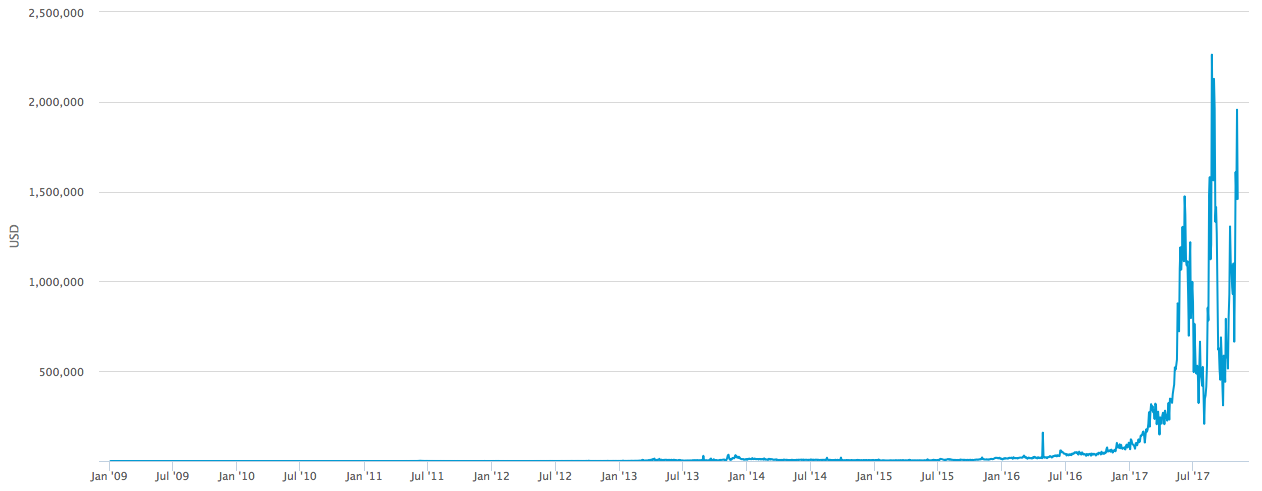
\includegraphics  [scale=0.25]{Images/transaction-fees}
		\caption{	Total value of all Bitcoin transaction fees paid to miners}
	\end{figure}
	\begin{tiny}
		Source: blockchain.info
	\end{tiny}
\end{frame}

% -----------------------------------------------------------------

\begin{frame}{Block reward}
	\begin{itemize}
		\item Processing nodes (miners) are offered a block reward as an additional incentive for securing the blockchain
		\item This is a reward in the form of newly generated cryptocurrency, that is given to the miner that successfully posts a valid block
		\item The value of the reward is determined by the architecture of the blockchain
		\item The Bitcoin reward started at 50BTC in the first block and halves every 210000 blocks ($\approx$ 4 years). It is currently 12.5BTC
		\item Ethereum offers a static block reward of 3 Ether
	\end{itemize}
\end{frame}


% -----------------------------------------------------------------

\begin{frame}{Coinbase transactions}
	\begin{itemize}
		\item The block reward is assigned using a coinbase transaction
		\item This is a special type of transaction used to create new units of the cryptocurrency
		\item Each block will contain one and only one coinbase transaction to reward the block miner, and it must be the first transaction of the block
		\item Coinbase transactions are the only transactions without real inputs as they are not linked to any previous transaction
	\end{itemize}
\end{frame}

% -----------------------------------------------------------------

\begin{frame}{Coinbase transactions}
	\begin{itemize}
		\item The coinbase transaction can have an arbitrary input of 100 byte size. E.g. the Bitcoin genesis block coinbase parameter contained the newspaper  headline "The Times 03/Jan/2009 Chancellor on brink of second bailout for banks", probably believed to be proof that the block was created on or after January 3, 2009
		\item The transaction's output is used to send the block reward and transaction fees to the miners address
		\item The k-block rule applies to these transactions i.e. Bitcoin's coinbase transactions cannot be spent until they have received at least 100 confirmations on the blockchain ($\approx$ 16hrs 40min)
		\item This prevents double spending in the event of a fork (i.e. a split) in the chain
	\end{itemize}
\end{frame}

% -----------------------------------------------------------------

\begin{frame}
	\begin{scriptsize}
	\end{scriptsize}
	\begin{figure}[]
		\centering
		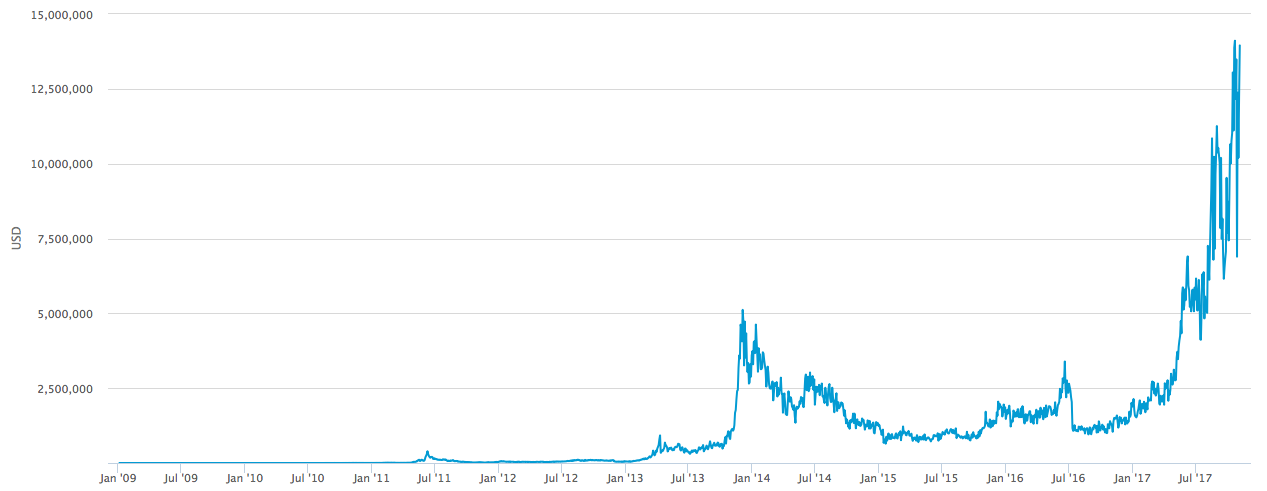
\includegraphics  [scale=0.25]{Images/miners-revenue}
		\caption{Total value of Bitcoin block rewards and transaction fees paid to miners}
	\end{figure}
	\begin{tiny}
		Source: blockchain.info
	\end{tiny}
\end{frame}

% -----------------------------------------------------------------

\begin{frame}{Bitcoin transaction ledger}
	\begin{figure}[]
		\centering
		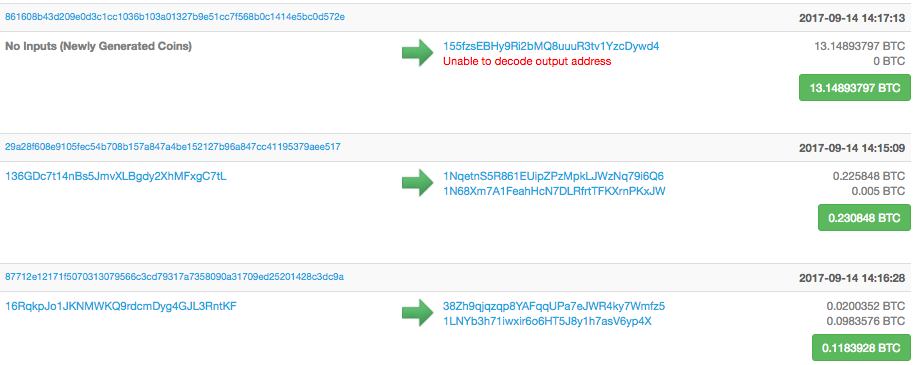
\includegraphics  [scale=0.3]{Images/trans}
	\end{figure}
	\begin{tiny}
		Source: blockchain.info
	\end{tiny}
\end{frame}

% -----------------------------------------------------------------

\begin{frame}{Blockchain anatomy}
	\begin{figure}[]
		\centering
		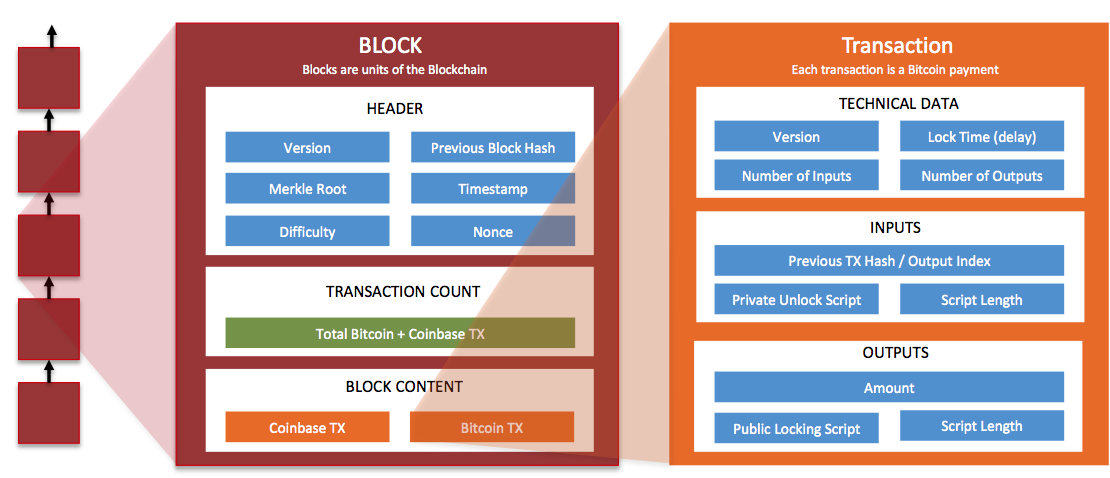
\includegraphics  [scale=0.5]{Images/anatomy}
	\end{figure}
	\begin{tiny}
		Source: \href{https://www.slideshare.net/arcatomia/anatomy-of-a-blockchain}{https://www.slideshare.net/arcatomia/anatomy-of-a-blockchain}
	\end{tiny}
\end{frame}

% -----------------------------------------------------------------

\begin{frame}{Broadcasting transactions}
	\begin{itemize}
		\item Peers will exchange information until it is available to every node on the network
		\item When a transaction is executed on a node and its validity is confirmed, the node stores it and then announces it to its nearest neighbors
		\item The neighbor nodes will in turn confirm the validity of the transaction and broadcast the transaction information to their respective neighbors
		\item This process goes on until the transaction is propagated across the network
		\item Transmission across the entire Bitcoin network takes 1-2 seconds
	\end{itemize}
\end{frame}


% -----------------------------------------------------------------

\begin{frame}{Broadcasting transactions}
	\begin{figure}[]
		\centering
		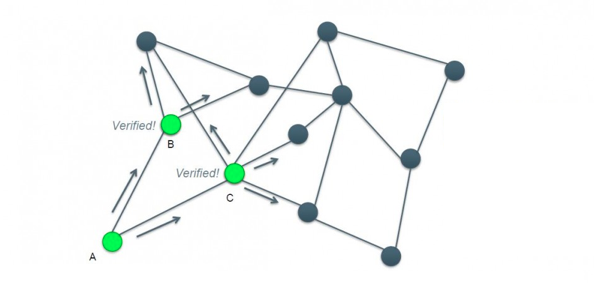
\includegraphics  [scale=0.4]{Images/broadcast}
		\caption{Node A announces a transaction to its peers B and C. If the transaction is verified, B and C announce it to their peers}
	\end{figure}
\end{frame}

	%https://www.actuaries.digital/2015/04/24/bitcoins-banking-and-the-blockchain/

% -----------------------------------------------------------------

\subsection{Consensus}

\begin{frame}{Consensus}
	\begin{itemize}
		\item Consensus is a process of agreement between distrusting nodes on a final state of data
		\item To maintain the transaction ledger, blockchains use distributed consensus i.e. consensus is achieved between multiple nodes on the network
		\item A consensus mechanism describes the set of steps that are taken by all, or most, nodes in order to agree on a proposed state of the data
		\item In order to achieve the desired outcome, a consensus mechanism must meet the following requirements
		\begin{enumerate}
			\item Agreement
			\item Termination
			\item Validity
			\item Byzantine fault tolerant
			\item Integrity
		\end{enumerate}
	\end{itemize}
\end{frame}

% -----------------------------------------------------------------

% \begin{frame}{Consensus}
% 	In order to achieve the desired outcome, a consensus mechanism must meet the following requirements
% 	\begin{itemize}
% 		\item Agreement - all nodes must decide on the same values
% 		\item Termination - all honest nodes terminate execution of the consensus process and eventually reach a decision
% 		\item Validity - the value agreed upon by all honest nodes must be the same as the initial value proposed by at least one honest node
% 		\item Byzantine fault tolerant - the consensus algorithm should be able to run in the presence of faulty or malicious nodes i.e. Byzantine nodes
% 		\item Integrity - each nodes makes a decision only once in a single consensus cycle
% 	\end{itemize}
% \end{frame}

% -----------------------------------------------------------------

\begin{frame}{Consensus}
	\begin{figure}[]
		\centering
		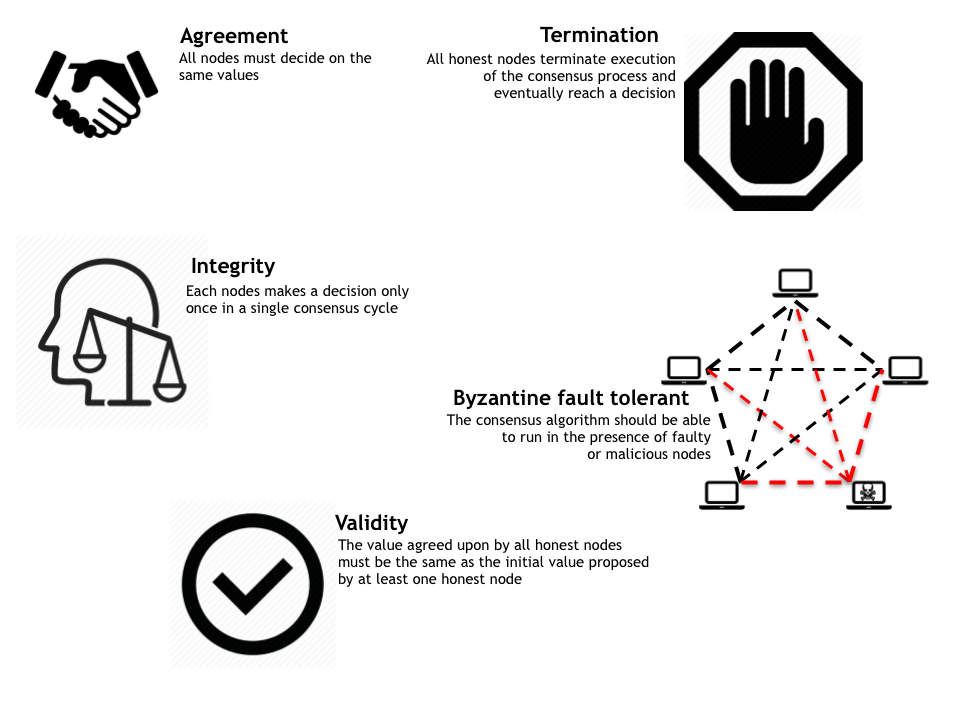
\includegraphics  [scale=0.3]{Images/consensus-req}
	\end{figure}
\end{frame}

% -----------------------------------------------------------------

\begin{frame}{Byzantine Generals' Problem}
	\begin{figure}[]
		\centering
		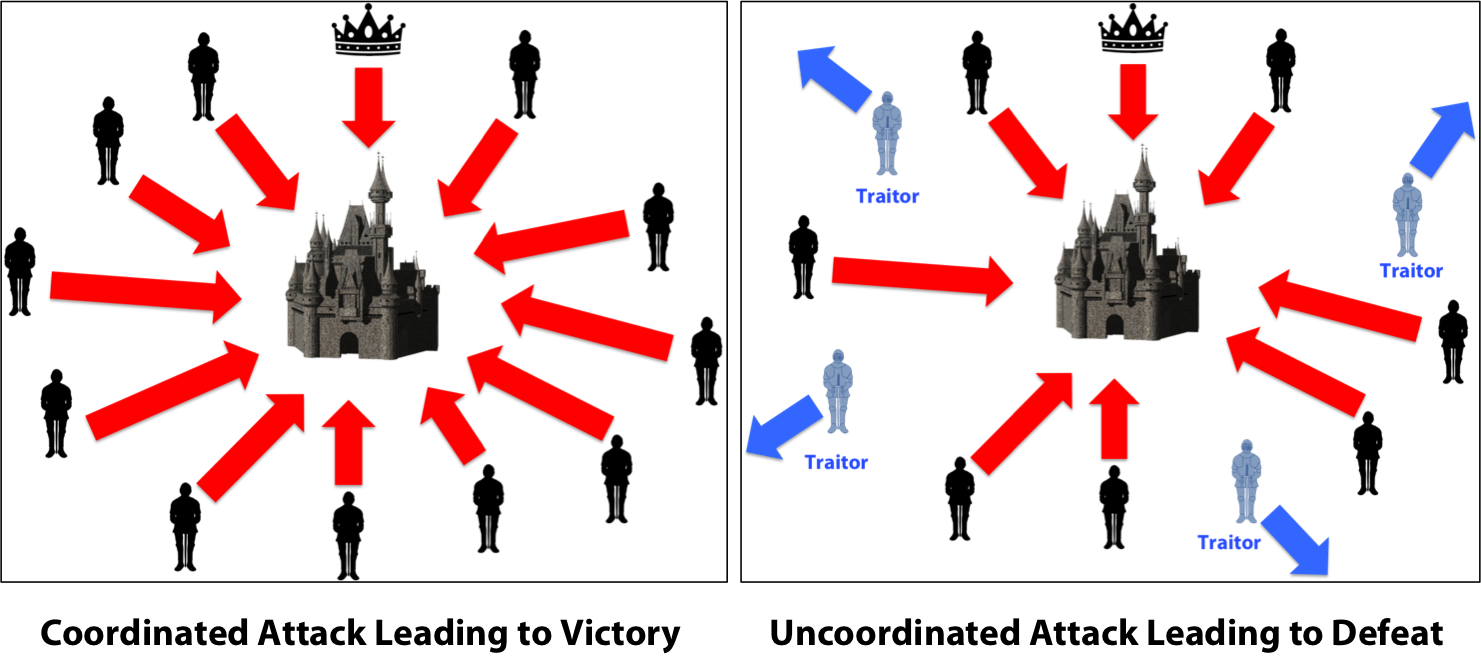
\includegraphics  [width=4.in]{Images/byzantine}
	\end{figure}
	\begin{tiny}
		Source: \href{https://cdn-images-1.medium.com/max/800/0*-xCD-El4LZ48dji1.png}{https://cdn-images-1.medium.com/max/800/0*-xCD-El4LZ48dji1.png}
	\end{tiny}
\end{frame}

% -----------------------------------------------------------------


\begin{frame}{Byzantine Generals' Problem}
	\begin{itemize}
		\item An agreement problem in which a group of generals, each commanding a portion of the Byzantine army, encircle a city
		\item In its simplest form, the generals only need to reach consensus on whether to attack or retreat
		\item For a halfhearted attack by a few generals would become a rout and be worse than a coordinated attack or a coordinated retreat
		\item A Byzantine failure is defined as an arbitrary deviation of a process from its assumed behavior based on the algorithm it is supposed to be running and the inputs it receives
		\item Byzantine fault tolerance is therefore achieved if all loyal generals are able to reach a unanimous agreement on their strategy
		\item And if every loyal general does not deviate from that common decision as a result of the influence of traitorous generals
	\end{itemize}
\end{frame}


% -----------------------------------------------------------------

\begin{frame}{Byzantine Fault Tolerance}
	\begin{itemize}
		\item Formally, the conditions for a consensus protocol tolerating Byzantine failures are
		\begin{itemize}
			\item Termination - every non faulty process (participant) decides on some value
			\item Validity - If all non faulty processes propose the same value, then all correct processes decide on that exact value
			\item Integrity - The value that has been decided on must have been proposed by some process
			\item Agreement - Every non faulty process must agree on the same value
		\end{itemize}
	\end{itemize}
\end{frame}

% -----------------------------------------------------------------

\begin{frame}{Byzantine Fault Tolerance}
	\begin{itemize}
		\item The ability to tolerate byzantine failures is a crucial part of a blockchain's ability to maintain reliable records of transactions in a transparent, tamper-proof way
		\item The need for trust when transacting on a network, that is borne out of fear of malicious entities, is eliminated given that the integrity of the system can be maintained even in the presence of these entities
		\item This allows users to transact in a hostile environment
		\item Fundamentally, BFT systems assign a threshold for consensus, by way of the system allowing for a proportion of processes to fail (reject consensus) and still achieve consensus, before the whole system fails
	\end{itemize}
\end{frame}

% -----------------------------------------------------------------

\begin{frame}{Sybil attacks}
	\begin{itemize}
		\item Traditional blockchain implementations have at a 50\% threshold before the integrity of the system can be compromised (i.e. 51\% attack)
		\item  Because many distributed systems have no form of identity management beyond accounts that are trivially created, such a system would be at risk of a Sybil attack
		\item In a Sybil attack the attacker challenges the integrity of a peer-to-peer network by creating a large number of pseudonymous identities, using them to gain a disproportionately large influence
		\item A Sybil attacker would therefore have to control at least 50\% of the processes in order to pose a threat
	\end{itemize}
\end{frame}

% -----------------------------------------------------------------

\begin{frame}{Sybil attacks}
	\begin{figure}[]
		\centering
		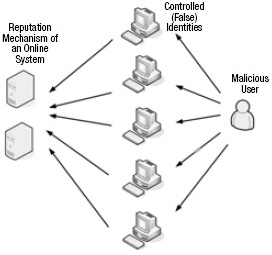
\includegraphics  [scale=0.5]{Images/sybil}
		\caption{A malicious user assumes multiple identities on the network in an attempt to undermine the integrity of the decision making process}
	\end{figure}
	\begin{tiny}
		Source: \href{https://www.isaca.org/Journal/archives/2010/Volume-4/Pages/JOnline-Auditing-Electronic-Auction-Systems.aspx}{https://www.isaca.org/Journal/archives/2010/Volume-4/PublishingImages/10v4auditing-electronic.jpg}
	\end{tiny}
\end{frame}

% -----------------------------------------------------------------

\begin{frame}{Proof of Work}
	\begin{itemize}
		\item Sybil attacks are avoided in Bitcoin by requiring block generation ability to be proportional to computational power available through the Proof-of-Work (PoW) consensus mechanism
		\item A proof-of-work system involves solving a complex puzzle to create a new block
		\item The creation of blocks is made difficult by the puzzle, which requires a significant amount of computational power to solve
		\item The process of creating blocks in the proof-of-work system is called mining
	\end{itemize}
\end{frame}
% -----------------------------------------------------------------

\begin{frame}{Proof of Work}
	\begin{itemize}
		\item To solve the puzzle, nodes must find a nonce that that can be used to generate a valid block
		\item A block will only be valid, if it hashes to value smaller than the hash of the previous block i.e. the new block must have been more difficult to compute
		\item This is achieved by manipulating the nonce until the new block's hash satisfies this condition i.e. the nonce is used as proof that sufficient labor has been undertaken
		\item SHA256 is used as the underlying cryptographic hash function
		\end{itemize}
\end{frame}

	% Nakamoto's design uses the Proof of Work consensus mechanism to verify the validity of a block i.e. the node posting a new block has to prove that sufficient labor was undertaken when computing the value of the nonce\\ \vspace{3mm}
	% 	Consensus on the validity of a block is therefore determined by the majority computational power on the network \\ \vspace{3mm}
	% 	%The use of distributed consensus is what allows for activity to occur in this hostile environment of conflicting interests, as it removes the need for trust between transacting parties\\ \vspace{3mm}
	% 	 and once more than 50\% of the mining nodes do this, consensus is considered as reached

% -----------------------------------------------------------------

\begin{frame}{Proof of Work}
	\begin{itemize}
		\item This design makes the entire process inherently resource intensive, providing strong cryptographic guarantees of Sybil resilience.
		\item If a malicious node decides to alter some transactions in a previous block, then the node will need to compute a nonce for all the succeeding blocks
		\item By the time it re-finds the nonce of all the succeeding blocks, more blocks would have been mined, making it infeasible to edit the history of a blockchain
		\item Furthermore, this fraudulent blockchain would be rejected as on the basis that its combined difficulty would be lower than the current chain
	\end{itemize}
\end{frame}

% ------------------------------------------------------------------

\begin{frame}{Proof of Work}
	\begin{itemize}
		\item However there is no guarantee that the node with the highest hash rate will always find the nonce first, due to the randomness involved in the process
		\item A higher hashrate only means the node can make attempts at finding the nonce at a faster rate
		\item The hash of the block being mined will be different for every miner because the has depends on variable factors like the time stamp and the miners address
		\item As a result, the nonce will be different for every miner
		\item Therefore, it's not a race to solve the puzzle; rather, it's a lottery system where the likelihood of getting lucky is determined by the miner's hash power
	\end{itemize}
\end{frame}

% -----------------------------------------------------------------

\begin{frame}{Proof of Work}
	\begin{figure}[]
		\centering
		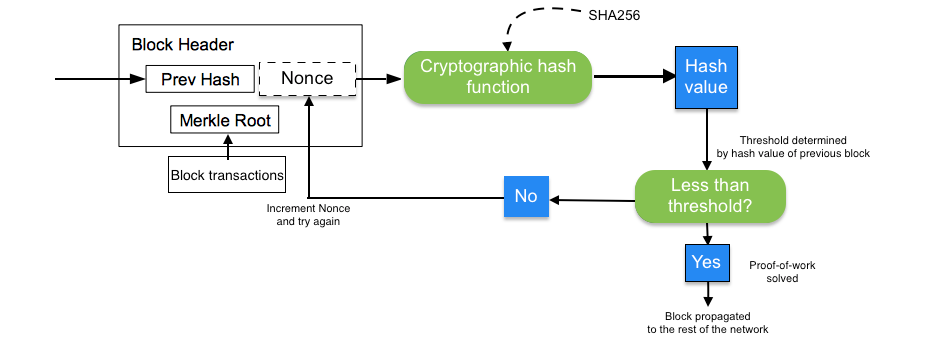
\includegraphics  [scale=0.35]{Images/pow}
	\end{figure}
\end{frame}

% ------------------------------------------------------------------

\begin{frame}{Achieving consensus}
	Once a 'solution' has been found, nodes do not explicitly express their acceptance of a new block\\ \vspace{3mm}
	Instead, consensus is implied by the nodes moving on to 'solve' the next block, with a header that points to the recently accepted block as the previous block in the chain\\ \vspace{3mm}
	Consensus is not guaranteed; failure to achieve it could result in a 'fork' in the blockchain i.e a split in the chain where nodes start operating on different versions of the chain
\end{frame}

% -----------------------------------------------------------------

\begin{frame}{Forking}
	\begin{itemize}
		\item A fork happens when there is a conflict among nodes regarding the validity of a blockchain
		\item When more than one blockchain exists on the network and every blockchain is validated for some miners
		\item Three types of forks exist: A regular fork, soft fork and a hard fork
	\end{itemize}
\end{frame}

% -----------------------------------------------------------------

\begin{frame}{Forking}
	\begin{figure}[]
		\centering
		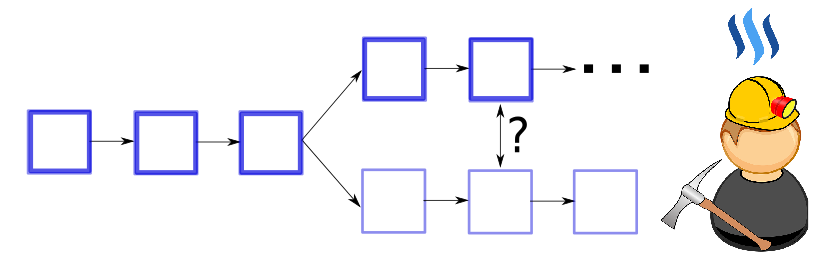
\includegraphics  [scale=0.1]{Images/fork6}
	\end{figure}
	\begin{tiny}
		Source: \href{https://steemkr.com/blockchain/@rtrader/blockchain-split-soft-vs-hard-fork}{https://steemitimages.com/DQmb6KJRQfAwHxQdFbAhrqMq2ZdWSQ9v7687tHViG3EEXpD/chain.png}
	\end{tiny}
\end{frame}

% -----------------------------------------------------------------

\begin{frame}{Forking}
	\begin{enumerate}
		\item Regular fork/ chain split: A temporary fork that happens when two miners find a block at nearly the same time. Resolved by coordination among the miners
		\item Soft fork: Happens when a change to the software protocols invalidates a subset of old blocks/transactions
		\begin{itemize}
			\item This type of fork is forward compatible i.e. all blocks considered valid by the newer version are also valid in the old version
			\item If majority hash power shifts to the newer version, the system will self correct
		\end{itemize}
		\item Hard fork: A change in software protocols that requires all miners to upgrade in order to resolve the conflict
		\begin{itemize}
			\item Hard forks are not forward compatible as previously invalid blocks become valid
			\item Older versions will not accept the new blocks, causing the users of the old software to remain on their own blockchain fork indefinitely
		\end{itemize}
	\end{enumerate}
\end{frame}

	%https://bitcoin.stackexchange.com/questions/30817/what-is-a-soft-fork

% -----------------------------------------------------------------

\begin{frame}{Soft vs hard forks}
	\begin{figure}[]
		\centering
		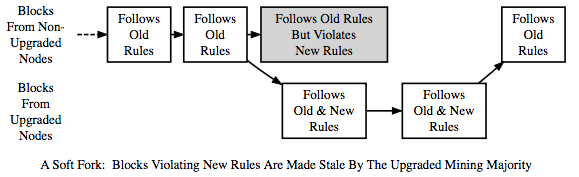
\includegraphics  [scale=0.4]{Images/soft-fork}
	\end{figure}
	\begin{figure}[]
		\centering
		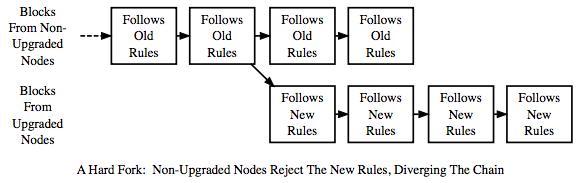
\includegraphics  [scale=0.4]{Images/hard-fork}
	\end{figure}
	\begin{tiny}
		Source: \href{https://bitcoin.org/en/developer-guide}{https://bitcoin.org/en/developer-guide}
	\end{tiny}
\end{frame}

% -----------------------------------------------------------------

\begin{frame}{Coordination in mining}
	Mining as a coordination game
	\begin{itemize}
		\item A direct result of the consensus mechanism is that mining becomes a coordination game
		\item Longest chain rule (LCR): Nodes will always consider the longest chain to be the canonical one and will keep working on extending that chain
		\item Theoretically, if miners follow this rule, there will be no forks and only a single chain
		\item In practice forks sometimes occur, and consensus temporarily disappears
	\end{itemize}
\end{frame}

	%https://bitcoin.stackexchange.com/questions/5540/what-does-the-term-longest-chain-mean

% -----------------------------------------------------------------

\begin{frame}{Longest chain rule}
	To understand the significance of LCR consider the following scenario
	\begin{itemize}
		\item Suppose two miners both find valid blocks within a few seconds of each other and broadcast them to the network. This is entirely feasible, given that it is a peer to peer network
		\item And because the network is global, latency will result in some nodes seeing the first miner's block and others will see the second
		\item Now there are two chains with identical history up until this point, and neither is longer than the other, resulting in a temporary fork
		\item Eventually another miner will find the next valid block, which will be attached to either one of the the chains
		\item This becomes the longest chain, and it becomes the definitive blockchain
		\item Transactions in the alternate fork do not disappear, they get put back in the pool of unconfirmed transactions and wait to be put in subsequent blocks
	\end{itemize}
\end{frame}

% -----------------------------------------------------------------

\begin{frame}{Longest chain rule}
	\begin{figure}[]
		\centering
		\includegraphics  [scale=0.5]{Images/lcr}
	\end{figure}
	\begin{tiny}
		Source: \href{https://shiftnrg.nl/docs/basic-knowledge/blockchain/what-are-blockchains-problems}{hhttps://shiftnrg.nl/wp-content/uploads/2017/05/start-mining-on-longest-1024x382.jpg}
	\end{tiny}
\end{frame}

% -----------------------------------------------------------------

\begin{frame}{Coordination in mining}
	\begin{itemize}
		\item Coordination is required, as each miners will want to attach their blocks to the chain to which they expect the others will attach their blocks
		\item And because of the k-block rule, each miner will have a vested interest in the survival of that chain in order to protect the value of their block rewards
		\item Miners decisions of which chain to mine are therefore strategic complements (i.e. they mutually reinforce one another)
	\end{itemize}
\end{frame}


% -----------------------------------------------------------------

\begin{frame}{Coordination in mining}
	\begin{itemize}
		\item Bitcoin's protocol uses a winner takes all reward scheme
		\item Hence miners will always try to avoid forks as there's the risk of loss of block rewards
		\item If a miner posts a valid block that is subsequently rejected after the fork has been resolved (i.e. a stale block), he has no loss protection from this
		\item Essentially, it is game theoretically optimal for every miner to mine on the longest chain and avoid mining forks
	\end{itemize}
\end{frame}

% -----------------------------------------------------------------

\begin{frame}{Stale blocks}
	\begin{itemize}
		\item The total number of stale blocks produced in the network is inversely proportional to the average time it takes to generate a new block
		\begin{itemize}
			\item Shorter block generation time means less time for the newly mined block to propagate throughout the network, increasing the probability of more than one miner finding a valid block, thereby creating stales
			\item If the average block generation time is longer, there is less chance that multiple miners will be able to find a valid block, increasing the time for the first solved block to be propagated across the network
		\end{itemize}
		\item The problem with stale blocks is that they may delay the confirmation of a transaction, as when two miners post a block at the same time, they won't necessarily always include the same set of transactions
		\item Hence the average confirmation time is not equal to average block generation time
	\end{itemize}
\end{frame}

% -----------------------------------------------------------------

\begin{frame}{Stale blocks}
	\begin{figure}[]
		\centering
		\includegraphics  [scale=0.4]{Images/stale}
	\end{figure}
	\begin{tiny}
		Source: \href{https://bitcoin.org/en/developer-guide}{https://bitcoin.org/en/developer-guide}
	\end{tiny}
\end{frame}

% -----------------------------------------------------------------

\begin{frame}{Stale blocks}
	\begin{itemize}

		\item Stale blocks also have the effect of incentivizing pooled mining, as miners try to avoid wasting computational effort
		\item Ethereum tackles the issues caused by stale blocks using a modified version of the GHOST (Greedy Heaviest Observed Subtree) protocol
		\item GHOST originally was a protocol modification, a chain selection rule, that makes use of blocks that are off the main chain to obtain a more secure and scalable system
		\item With this modification, it would be possible to speed up the blockchain to a velocity of up to 1 block per second, increasing the possible transaction rate without compromising the blockchain consensus and security
		\item This protocol is the reason why, relative to Bitcoin, Ethereum can achieve shorter block times while reducing the incentive for pooled mining
	\end{itemize}
\end{frame}

	% \item Forks also undermine the security of a blockchain
	% \item When the network parts and miners work on multiple blockchains, there is also a split in the hash power of the network as some of it is working on something that will eventually become unnecessary, thereby undermining the security of a blockchain

% -----------------------------------------------------------------

\begin{frame}{GHOST protocol}
	Ethereum refers to stale blocks as uncle blocks and its implementation of the GHOST protocol is defined as follows
	\begin{itemize}
		\item A block must specify a parent, and it must specify 0 or more uncles
		\item An uncle included in a block B must have the following properties:
		\begin{itemize}
			\item It must be a direct child of the $k^{th}$ generation ancestor of B, where $2 \leq k \leq 6$
			\item It cannot be an ancestor of B
			\item An uncle must be a valid block header, but does not need to be a previously verified or even valid block
			\item An uncle must be different from all uncles included in previous blocks and all other uncles included in the same block
		\end{itemize}
		\item For every uncle U in block B, the miner of B gets an additional 3.125\% added to its coinbase reward and the miner of U gets 93.75\% of a standard coinbase reward
	\end{itemize}
\end{frame}

% -----------------------------------------------------------------

\begin{frame}{Uncle mining}
	\begin{itemize}
		\item A maximum of 2 uncles are allowed per block
		\item The inclusion of uncle blocks has two main effects
		\begin{itemize}
			\item It decreases the incentive for centralization in the form of mining pools by removing the effects of network lag on dispersion of mining rewards as producers of stale blocks are still rewarded
			\item It increases the security of the chain by augmenting the amount of work on the main chain by that done in the uncles i.e. the overall difficulty of the blockchain also includes the sum of difficulties of the stale blocks
		\end{itemize}
		\item However, uncle mining also introduces additional economic complexity as some miners now have an incentive to mine empty uncles
	\end{itemize}
\end{frame}

% -----------------------------------------------------------------

\begin{frame}{Mining hardware}
	\begin{itemize}
		\item CPU mining was the first type of mining available in the original bitcoin blockchain, however this quickly became obsolete as nodes switched to GPU mining
		\item GPUs support faster and parallelized calculations, but even these did not last long
		\item Miners started using Field Programmable Gate Arrays (FPGAs), integrated circuits programmed to perform SHA256 calculations
		\item Eventually miners started using Application Specific Integrated Circuits (ASICs) designed to perform the SHA256 operation at a very high hashing rate
		\item Due to the quickly increasing mining difficulty level, single-unit ASICs are no longer profitable
	\end{itemize}
\end{frame}

% -----------------------------------------------------------------

\begin{frame}{Mining hardware}
	\begin{figure}[]
		\centering
		\includegraphics  [scale=0.2]{Images/hardware}
		\caption{Bitcoin relative mining difficulty chart with logarithmic vertical scale. Relative difficulty defined as 1 at 9 January 2009. Higher number means higher difficulty}
	\end{figure}
	\begin{tiny}
		Source: \href{https://commons.wikimedia.org/wiki/File:History_of_Bitcoin_difficulty_and_mining_hardware.svg}{https://commons.wikimedia.org/wiki/File:History\_of\_Bitcoin\_difficulty\_and\_mining\_hardware.svg}
	\end{tiny}
\end{frame}

% -----------------------------------------------------------------

\begin{frame}{Achieving consensus}
	\begin{itemize}
		\item It is possible to use alternative consensus mechanisms that are less centralized and more energy-efficient
		\item This includes Proof of Stake, Proof of Activity, Threshold signature schemes, Proof of Burn
		\item Multiple game theoretic considerations are feasible; with the caveat that the system has to be Byzantine fault tolerant
		\item However, each method will have its own advantages over the others that will make it more desirable, depending on the intended function of the blockchain
	\end{itemize}
\end{frame}

% -----------------------------------------------------------------

\begin{frame}{Alternative consensus mechanisms}
	Proof of stake
	\begin{itemize}
		\item Likelihood of updating the chain is determined by the wealth of the node.
		\item The definition of wealth is subjective and depends on the function of the blockchain e.g. value of currency or assets linked to the node
		\item This system works on the idea that if a node or user has enough stake in the system, acting truthfully would outweigh the benefits of performing an attack on the system
		\item The model aims to provide the same type of fairness in the distribution of the right to create a block without requiring miners to burn external resources
		\item Proof of stake systems are more decentralized, however they must work hard to build communities built around their tokens
	\end{itemize}
\end{frame}

% -----------------------------------------------------------------

\begin{frame}{Alternative consensus mechanisms}
	Proof of stake
	\begin{itemize}
		\item There are no block rewards, instead incentives for miners lie in wanting to guard their own wealth given that they have a vested interest in maintaining the integrity of the blockchain
		\item This design has been criticized for the fact that the wealthiest nodes will always stand to benefit the most from the transaction fees
		\item The concept of coin age can alleviate this; the probability of forging the next block reaches a maximum after an arbitrary number of days in order to prevent very old or very large collections of stakes from dominating the blockchain through centralized mining pools
	\end{itemize}
\end{frame}

% -----------------------------------------------------------------

\begin{frame}
	\begin{figure}[]
		\centering
		\includegraphics  [scale=0.15]{Images/vs}
	\end{figure}
	\begin{scriptsize}
		source: \href{https://blockgeeks.com/guides/proof-of-work-vs-proof-of-stake/}{https://blockgeeks-assets.scdn7.secure.raxcdn.com/wp-content/uploads/2017/03/infographics2017-01.png}
	\end{scriptsize}
\end{frame}

% -----------------------------------------------------------------

\begin{frame}{Alternative consensus mechanisms}
	Threshold signature schemes
	\begin{itemize}
		\item Uses a multi-signature scheme with a subset of nodes that can be tolerated to fail or be corrupted before the system fails
		\item The ability to construct a single signature used to sign a valid block is distributed across the network, with each node producing only a partial signature
		\item Consensus on an update is considered to be reached if the signature threshold $k$ has been met i.e.  $k$ out of $n$ signing nodes have generated valid signatures
		\item The rest of the $n-k$ participating nodes can can fail to deliver any or can deliver invalid signature shares
	\end{itemize}
\end{frame}

% -----------------------------------------------------------------

\begin{frame}{Alternative consensus mechanisms}
	Threshold signature schemes
	\begin{itemize}
		\item Desired network latency and tolerance to network failure will determine the value of n
		\item k will vary with the desired tolerance to Byzantine failures
		\item In a round robin fashion, nodes will take turns to create the next block within a specified time frame, to allow for the communication required to create the multi-signature to take place
		\item While significantly less resource intensive relative to the other consensus models, it reintroduces the requirement of trust
	\end{itemize}
\end{frame}

% -----------------------------------------------------------------

\begin{frame}{Alternative consensus mechanisms}
	Reputation based schemes
	\begin{itemize}
		\item The node to post the next block is selected on the basis of the reputation it has built over time
		\item This can be based on the voting of other member nodes
	\end{itemize}
	Federated byzantine consensus
	\begin{itemize}
		\item Nodes keep a group of publicly trusted peers and propagate only those transactions that have been validated by the majority of trusted nodes
		\item In turn, those trusted nodes do not agree to the transaction until the nodes they consider important agree as well, and so on
	\end{itemize}
\end{frame}

% -----------------------------------------------------------------

\begin{frame}{Alternative consensus mechanisms}
	Proof of burn
	\begin{itemize}
		\item The idea is that miners should show proof that they burned some coins i.e. sent them to a verifiably unspendable address
		\item This is intended such that an individual miner finds the task expensive, without consuming real resources
	\end{itemize}
	Proof of activity
	\begin{itemize}
		\item Designed as a combination of Proof of Work and Proof of Stake
		\item The nodes responsible for singing the next block are identified using a routine called \textit{follow-the-satoshi}
		\item N satoshis (smallest unit of the cryptocurrency) are chosen at random from the available supply. The N addresses identified as those that control these satoshis are then given the right to each sign the block header and a block will be valid only if all N addresses have signed it
	\end{itemize}
\end{frame}

% -----------------------------------------------------------------

\subsection{Digital tokens}

\begin{frame}{Digital tokens}
	\begin{itemize}
		\item Blockchains have the ability to store on them digital tokens
		\item These tokens exist conceptually as entries in the ledger
		\item You own these tokens because you have a key that lets you create a new entry re-assigning the ownership to someone else
		\item These can be used to represent assets such as USD or gold to company stocks, individual tokens representing smart property, secure unforgeable coupons, and even token systems with no ties to conventional value at all, used as point systems for incentivization
	\end{itemize}
\end{frame}

% -----------------------------------------------------------------

\begin{frame}{Digital tokens}
	Two types of digital tokens can be issued on a blockchain
	\begin{enumerate}
		\item Intrinsic tokens
			\begin{itemize}
				\item These are also called native tokens
				\item They are not backed by anything and their utility lies within the token itself
				\item The value of these tokens is determined within the system that they are created, by the people who own them e.g. cryptocurrencies
			\end{itemize}
		\item Asset backed tokens
			\begin{itemize}
				\item Represent claims to an underlying asset
				\item The tokens can be transferred from person to person and anyone holding the token can go back to the issuer and claim the underlying asset
				\item Unlike native tokens, these have no fungibility
			\end{itemize}
	\end{enumerate}
\end{frame}

% -----------------------------------------------------------------

\begin{frame}{Token rights}
	\begin{figure}[]
		\centering
		\includegraphics  [scale=0.35]{Images/token-rights}
	\end{figure}
\end{frame}

% -----------------------------------------------------------------

\subsection{How it works}


\begin{frame}{How it works}
	\begin{figure}[]
		\centering
		\includegraphics  [scale=0.25]{Images/infographic}
	\end{figure}
	\begin{scriptsize}
		source: \href{https://blockgeeks.com/guides/what-is-blockchain-technology/}{https://blockgeeks-assets.scdn7.secure.raxcdn.com/wp-content/uploads/2016/09/infographics0517-01-1.png}
	\end{scriptsize}
\end{frame}

% -----------------------------------------------------------------

\begin{frame}{How it works}
	The network runs in the following way
	\begin{enumerate}
		\item New transactions are validated and broadcast to all nodes.
		\item Each mining node collects new transactions into a block
		\item Mining nodes work on finding a difficult proof-of-work for their respective blocks
		\item When a node finds a valid block, it broadcasts it to its neighbors block to propagate across the network
		\item Nodes accept the block only if it has a valid block header
		\item Nodes express their acceptance of the block by working on creating the next block in the chain, using the hash of the accepted block as the new parent hash
	\end{enumerate}
\end{frame}

% -----------------------------------------------------------------

\begin{frame}{How it works}
	\begin{enumerate}
		\item New transactions are validated and broadcast to all nodes.
			\begin{itemize}
				\item Distributed databases require synchronicity in order to maintain a uniform record of information
				\item Once a transaction is executed by a node, it is broadcast to its nearest peers which in turn validate and then broadcast it to their nearest peers until the entire network has received the transaction details
				\item The validation process involves filtering out transactions not properly signed by private keys or transactions from accounts with insufficient balances
				\item After peers exchange their information they store it to be processed.
			\end{itemize}
	\end{enumerate}
\end{frame}

% -----------------------------------------------------------------

\begin{frame}{How it works}
	\begin{enumerate}
		\setcounter{enumi}{1}
		\item Each mining node collects new transactions into a block
		\begin{itemize}
			\item Miners collect all the new un-mined and valid transactions waiting to be confirmed and construct a merkle tree
			\item The miner creates a block, whose header contains the Merkle tree root of all the transactions, a timestamp, nonce, coinbase transaction and the hash of the parent block
			\item Using a Merkle tree is preferable over a hash chain or a hash of concatenated transactions because it allows for a much quicker and simpler test of whether a particular transaction is included in the set
		\end{itemize}
	\end{enumerate}
\end{frame}

% -----------------------------------------------------------------

\begin{frame}{How it works}
	\begin{enumerate}
		\setcounter{enumi}{2}
		\item Mining nodes work on finding a difficult proof-of-work for their respective blocks
		\begin{itemize}
			\item This step of finding a valid block varies with the consensus mechanism used
			\item The nonce is used as the proof-of-work and since finding valid one is computationally expensive, nodes are compensated for their efforts if successful
			\item Mining nodes are incentivised by being offered a 'block reward' in addition to the fees generated by the transactions in that block
		\end{itemize}
	\end{enumerate}
\end{frame}

% -----------------------------------------------------------------


\begin{frame}{How it works}
	\begin{enumerate}
		\setcounter{enumi}{3}
		\item When a node finds a valid block, it broadcasts it to its neighbors block to propagate across the network
		\item Nodes accept the block only if it has a valid block header
		\begin{itemize}
			\item A block is valid only if it hashes to a value less than the parent block and this can be checked by any node
			\item Validity can further be confirmed by checking whether the transactions in the block are valid, the block's timestamp or if the miner has assigned a block reward
		\end{itemize}
		\item Nodes express their acceptance of the block by working on creating the next block in the chain, using the hash of the accepted block as the new parent hash.
	\end{enumerate}
\end{frame}

% -----------------------------------------------------------------

\subsection{Blockchains outside of finance}

\begin{frame}{Blockchains outside of finance}
	A number of use cases of blockchains have been emerged across different industries since the technology's introduction \\ \vspace{3mm}
	This includes but is not limited to the Internet of Things, recording of events, medical records, identity management or any type of data that needs tracking \\ \vspace{3mm}
	Many of the leaders in the cloud space have since started offering blockchain solutions to their customers.
	Microsoft (\href{https://azure.microsoft.com/en-us/solutions/blockchain/}{Azure}), IBM (\href{https://console.bluemix.net/catalog/services/blockchain/}{BlueMix}) and Amazon (\href{https://aws.amazon.com/marketplace/}{AWS}) are the the leaders in the space for Blockchain as a Service (BaaS)
\end{frame}

	%http://it.toolbox.com/blogs/mainframe-world/blockchain-as-a-service-76361

% -----------------------------------------------------------------

\begin{frame}{Blockchains outside of finance}
	Internet of Things
	\begin{itemize}
		\item The concept of connecting devices embedded with sensors, software and network connectivity to the internet which enables these devices to communicate and collect and exchange data
		\item  IoT allows objects to be sensed or controlled remotely across existing network infrastructure, creating opportunities for more direct integration of the physical world into computer-based systems
		\item This has led to concepts, such as wearables, smart homes, smart grids, smart connected cars, and smart cities, all based on the basic concept of an IoT device
		\item Blockchains are promising for IoT security for the same reasons they works for cryptocurrency; immutability of data and authentication protocols guarantee fast, low cost and secure peer-to-peer communication between devices
	\end{itemize}
\end{frame}

% -----------------------------------------------------------------

\begin{frame}
	\begin{figure}[]
		\centering
		\includegraphics  [scale=0.2]{Images/iot-ecosystem1}
	\end{figure}
	\begin{scriptsize}
		source: \href{https://acceleratingbiz.com/proof-point/internet-things-iot-overview-selected-devices/}{https://acceleratingbiz.com/wp-content/uploads/2017/08/Internet-of-Things.png}
	\end{scriptsize}
\end{frame}

% -----------------------------------------------------------------

\begin{frame}{Blockchains outside of finance}
	Cloud storage
	\begin{itemize}
		\item Blockchain technology is continually being developed in an attempt to address concerns regarding existing models of cloud-based storage which are all centralized solutions.
		\item The technology is being used to provide decentralized and distributed storage across communities instead of a single central organization
		\item Nodes avail storage space on their hard drives and are able to act autonomously to perform various functions such as data transfer, validation and perform data integrity checks
		\item Files are encrypted and divided into small pieces (shards) to be distributed across the network
		\item Participating nodes are typically compensated with cryptocurrency for their contribution to the storage space available on the network
	\end{itemize}
\end{frame}

% -----------------------------------------------------------------

\begin{frame}{Blockchains outside of finance}
	\begin{figure}[]
		\centering
		\includegraphics  [scale=0.3]{Images/storj}
		\caption{The sharding process}
	\end{figure}
		\begin{scriptsize}
		source: \href{https://decentralize.today/simplifying-the-storj-whitepaper-ef38ad0ea7de}{https://decentralize.today/simplifying-the-storj-whitepaper-ef38ad0ea7de}
	\end{scriptsize}
\end{frame}

% -----------------------------------------------------------------

\begin{frame}{Implementation challenges}
	\begin{figure}[]
		\centering
		\includegraphics  [scale=0.3]{Images/implementation}
	\end{figure}
\end{frame}

% -----------------------------------------------------------------

\begin{frame}{Streamlining existing markets}
	\begin{figure}[]
		\centering
		\includegraphics  [scale=0.3]{Images/savings}
	\end{figure}
\end{frame}

% -----------------------------------------------------------------

\begin{frame}{Blockchain consortiums}
	A handful of consortiums have also since emerged, with the intention of advancing the use of blockchains in the financial services industry
	\begin{itemize}
		\item R3
		\begin{itemize}
			\item A distributed database technology company that leads a consortium of more than 70 of the world's biggest financial institutions in blockchain research and development
			\item The consortium started on September 15, 2015 with nine financial companies, including Barclays, Credit Suisse, Goldman Sachs and J.P. Morgan
			\item Their flagship product is Corda, a distributed ledger platform designed for financial institutions to record, manage and automate legal agreements between business partners
			\item Although it is inspired by blockchain databases, and is expected to have many of the benefits of blockchains, it is not a blockchain
			\item Makes use of "supervisory observer nodes", which can be used by regulators to monitor the system
		\end{itemize}
	\end{itemize}
\end{frame}

% -----------------------------------------------------------------

\begin{frame}{Blockchain consortiums}
	\begin{itemize}
		\item Hyperledger
		\begin{itemize}
			\item An umbrella project of open source blockchains and related tools started in December 2015 by the Linux Foundation, with the objective of advance cross-industry collaboration and a focus on improving the performance and reliability of blockchains and distributed ledgers
			\item Early members include IBM, Intel, J.P. Morgan, Wells Fargo and SAP
			\item Has multiple blockchain platforms including Hyperledger Burrow, Hyperledger Fabric, Hyperledger Iroha and Hyperledger Sawtooth
			\item Hyperledger Fabric is a permissioned blockchain infrastructure, originally contributed by IBM and Digital Asset
			\item It provides a modular architecture with a delineation of roles between the nodes in the infrastructure, execution of Smart Contracts, and configurable consensus and membership services
		\end{itemize}
	\end{itemize}
\end{frame}

% -----------------------------------------------------------------

\begin{frame}{Blockchain consortiums}
	\begin{itemize}
		\item South African Financial Blockchain Consortium
		\begin{itemize}
			\item A collective of 24 institutions that have come together to explore the use of blockchain technology in the South African financial market
			\item Members include Capitec, the Reserve Bank of South Africa and UCT
			\item In addition to Ethereum, they are exploring the use of the Corda, Hyperledger and Chain Core platforms
			\item Primary objectives include reducing inefficiencies and creating opportunities to save costs for institutions and end consumers
			\item It also intends to explore using a permissioned distributed ledger to store identity information to alleviate administrative requirements and costs associated with Know-Your-Customer (KYC) and the Financial Intelligence Centre Act (Fica)
		\end{itemize}
	\end{itemize}
\end{frame}

	%https://www.moneyweb.co.za/news/tech/sa-takes-steps-to-set-up-national-financial-blockchain/

% -----------------------------------------------------------------

\begin{frame}{Recap}
	\begin{itemize}
		\item Blockchains reintroduce a form of single entry bookkeeping in financial services
		\item Cryptography is used to enable secure communication and guarantee overall security of the system
		\item The integrity of a blockchain depends on private keys remaining private
		\item There are multiple consensus mechanisms preferable over Proof-of-Work as they are significantly less resource intensive. The ideal choice ultimately depends on the desired function of the blockchain
		\item Ethereum makes use of the GHOST protocol to prevent wastage of resources that comes with mining stale blocks under Proof-of-work
		\item Two kinds of digital tokens can be issued on a blockchain; intrinsic tokens and asset backed tokens
	\end{itemize}
\end{frame}

% -----------------------------------------------------------------

\begin{frame}{Recap}
	\begin{figure}[]
		\centering
		\includegraphics  [scale=0.3]{Images/block-key}
		% \caption{}
	\end{figure}
\end{frame}

% -----------------------------------------------------------------

\begin{frame}{Recap}
	\begin{figure}[]
		\centering
		\includegraphics  [scale=0.3]{Images/benefits}
		% \caption{}
	\end{figure}
\end{frame}

% -----------------------------------------------------------------

\begin{frame}{Recap}
	\begin{figure}[]
		\centering
		\includegraphics  [scale=0.3]{Images/consensus}
		\caption{A basic consensus model}
	\end{figure}
\end{frame}

% -----------------------------------------------------------------

\section{Cryptocurrency}

\begin{frame}
	\begin{center}
		\begin{large}
			Cryptocurrency
		\end{large}
	\end{center}
\end{frame}

% -----------------------------------------------------------------


\begin{frame}{}
	\begin{itemize}
		\item A cryptocurrency is a form of digital cash issued on a blockchain platform
		\item Bitcoin was the first cryptocurrency launched in 2009 and since then well over 900 other cryptocurrencies have emerged
		\item Generally no two cryptocurrencies are alike as they all leverage blockchains in unique ways
		\item Some blockchain platforms allow users to issue their own cryptocurrency through the use of smart contracts
		\item Cryptocurrencies were designed with the intention of not having to require sovereign backing, however multiple central banks are looking to leverage the benefits of blockchains by developing their own digital currencies
	\end{itemize}
\end{frame}

% -----------------------------------------------------------------

\subsection{Cryptocurrency}

\begin{frame}{Currency}
	Currency is a generally accepted form of money that is accepted within an economy\\ \vspace{3mm}
	A sovereign state retains the right to decide which currency it shall use, therefore a currency will have limited boundaries of acceptance \\ \vspace{3mm}
	Modern financial systems evolved and have come to use fiat money\\ \vspace{3mm}
	This is a currency without intrinsic value, established as money by government regulation or law. It was introduced as an alternative to commodity money i.e. money created from precious metal such as gold or silver and hence intrinsically valuable
\end{frame}

% -----------------------------------------------------------------

\begin{frame}{Cryptocurrency}
	A decentralized digital currency that uses cryptography to regulate the issue of new units of the currency, to verify transactions and ownership of the currency and maintain the security of the system independent of a central authority
	\begin{figure}[]
		\centering
		\includegraphics  [width=2.in]{Images/cryptocurrency}
	\end{figure}
\end{frame}

% -----------------------------------------------------------------


\begin{frame}{Cryptocurrency}
	"Digital tokens like bitcoin, ethereum that are stateless, do not have sovereign endorsement, a qualified issuing body or a country's trust, are not legal currencies and should not be spoken of as digital currencies"- \begin{scriptsize}
	\textit{Li Lihui, former president of the Bank of China}
	\end{scriptsize}
\end{frame}

% -----------------------------------------------------------------


\begin{frame}{Cryptocurrency}
	\begin{itemize}
		\item As of July 2017 there were over 900 cryptocurrencies available online
		\item The combined value of all digital currencies stood at \$17.5bn at the start of 2017 and reached an all time high of \$150bn in August of the same year
		\item Prior to the existence of cryptocurrencies, peer-to-peer exchange was restricted to physical forms of money
	\end{itemize}
\end{frame}

% -----------------------------------------------------------------

\begin{frame}{Cryptocurrency}
	The main features of a cryptocurrency are
	\begin{enumerate}
		\item Has no intrinsic value that is redeemable for another commodity or asset of value
		\item Has no physical for and exists only on the network
		\item Supply is not determined by a central issuing authority and the network is completely decentralized
	\end{enumerate}
\end{frame}

% -----------------------------------------------------------------

\begin{frame}{Cryptocurrency}
	Some, but not all of the features of a cryptocurrency are also common to other forms of money
	\begin{itemize}
		\item Cash is peer-to-peer, but it is not electronic, and it is the liability of a central bank
		\item Commercial bank deposits are a liability of the bank that issues them and exchanged in a centralized manner either across the books of a given bank or between different banks via the central bank
		\item Commodity money may also be transferred in a peer-to-peer fashion but it is neither the liability of anyone nor electronic
	\end{itemize}
\end{frame}

% -----------------------------------------------------------------

\begin{frame}{Cryptocurrency}
	\begin{figure}[]
		\centering
		\includegraphics  [scale=0.3]{Images/markcap}
	\end{figure}
	*not mineable\\
	\begin{tiny}
		as at 12 Sept 2017
	\end{tiny}
\end{frame}

% -----------------------------------------------------------------


\begin{frame}{Cryptocurrency}
	\begin{figure}[]
		\centering
		\includegraphics  [width=3.in]{Images/price}
	\end{figure}
	\begin{scriptsize}
		source \href{https://www.tradingview.com}{https://www.tradingview.com}
	\end{scriptsize}
\end{frame}

% -----------------------------------------------------------------


\begin{frame}{Cryptocurrency}
	\begin{figure}[]
		\centering
		\includegraphics  [width=4.in]{Images/vol}
	\end{figure}
	\begin{scriptsize}
		source \href{https://www.buybitcoinworldwide.com/ethereum-volatility/}{https://www.buybitcoinworldwide.com/ethereum-volatility/}
	\end{scriptsize}

\end{frame}

% -----------------------------------------------------------------


\begin{frame}{Cryptocurrency}
	Unlike conventional currency, there is no issuing authority to regulate the supply in circulation \\ \vspace{3mm}
	The People's Bank of China has on multiple occasions made clear their discontentment with cryptocurrencies because of this\\ \vspace{3mm}
	In September 2017, Chinese authorities ordered Beijing-based cryptocurrency exchanges to stop trading and immediately notify users of their closure, in an attempt to contain financial risks \\ \vspace{3mm}
	Authorities cited concerns about illegal fund flows and limiting risks to consumers amid a highly speculative market that has grown rapidly
\end{frame}

% -----------------------------------------------------------------



\begin{frame}{Cryptocurrency}
		New units are typically issued in a deterministic way as currencies are either mined or pre-mined
	\begin{itemize}
		\item In the case of mined currencies, new units are created in the form of block rewards with the creation of new blocks e.g. Bitcoin, Ethereum, Litecoin
		\item 'pre-mined' currencies will have have a fixed supply from the inception of the blockchain and all the available coin will be active and readily available e.g. Ripple
		\item Most currencies are pre-mined to a certain extent. Developers and stake holders to do this to assure that if their project is very valuable they get a piece of it and at the same time avoid having a large percentage of the coin is in the hands of a few people in the long run.
	\end{itemize}
	Bitcoin (BTC), Ethereum (ETH) and Ripple (XRP) are the most relevant platforms in terms of their potential contribution to the financial services industry
\end{frame}

% -----------------------------------------------------------------

\subsection{Bitcoin}

\begin{frame}
	\begin{figure}[]
		\centering
		\includegraphics  [scale=0.1]{Images/bitcoin-logo}
	\end{figure}
\end{frame}

% -----------------------------------------------------------------

\begin{frame}{Bitcoin}
	\begin{figure}[]
		\centering
		\includegraphics  [scale=0.5]{Images/dilbert-bitcoin}
	\end{figure}
\end{frame}

% -----------------------------------------------------------------

\begin{frame}{Bitcoin}
	\begin{itemize}
		\item Introduced by Nakamoto in 2008 as a decentralized peer-to-peer electronic cash system
		\item The first viable, decentralized, reliable form of digital cash. Previous attempts include:
		\begin{itemize}
			\item e-cash, an anonymous cryptographic electronic cash system conceived by David Chaum in 1983
			\item B-money, an early proposal created by Wei Dai for an "anonymous, distributed electronic cash system" in 1998. Nakamoto referenced b-money when creating Bitcoin
			\item At the same time, Nick Szabo introduced BitGold, also based on the PoW mechanism
		\end{itemize}
		\item Operates on a public blockchain, with over 10000 functioning nodes worldwide
	\end{itemize}
\end{frame}

	% https://bitcoin.org/en/developer-guide#block-chain-overview

% -----------------------------------------------------------------

\begin{frame}{Bitcoin}
	\begin{itemize}
		\item Bitcoin can be defined in various ways; it is a protocol, a digital currency and a platform
		\item Supply of the currency is controlled and limited to 21million BTC. By July 2017, 16.4 million Bitcoins were in circulation; the smallest unit of measurement is a satoshi ($ 10^{-8}$BTC)
		\item The number of bitcoins generated per block is set to decrease geometrically, with a 50\% reduction every 210,000 blocks($\approx$ 4 years)
		\item It is estimated that by 2140, there will be no more Bitcoin left to mine and at that point, miners will only be incentivised by transaction fees
		\item Approximately 1800 Bitcoins are mined everyday
		\end{itemize}
\end{frame}

% -----------------------------------------------------------------

\begin{frame}{Bitcoin supply}
	\begin{figure}[]
		\centering
		\includegraphics  [scale=0.2]{Images/btc-circulation}
	\end{figure}
		\begin{scriptsize}
		source: \href{https://blockchain.info/charts/total-bitcoins?timespan=all}{https://blockchain.info/charts/total-bitcoins?timespan\=all}
	\end{scriptsize}
\end{frame}

% -----------------------------------------------------------------

\begin{frame}{Bitcoin}
	To date there is no clear regulatory stance on whether Bitcoin should be classified as investment or a currency \\ \vspace{3mm}
	Nonetheless many vendors and merchants already accept it as a form of payment
	\begin{itemize}
		\item In May 2010, a developer bought two pizzas using 10,000BTC worth \$41 at the time. Today the pizzas are worth more than \$31million
		\item Microsoft allows users to buy content with on Xbox and Windows store
		\item Tesla also accepts bitcoin as a method of payment
	\end{itemize}
\end{frame}

% -----------------------------------------------------------------

\begin{frame}{Bitcoin}
	\begin{figure}[]
		\centering
		\includegraphics  [width=3in]{Images/pizza1}
	\end{figure}
\end{frame}

% -----------------------------------------------------------------

\begin{frame}{Bitcoin}
	\begin{figure}[]
		\centering
		\includegraphics  [width=3in]{Images/pizza2}
	\end{figure}
\end{frame}

% -----------------------------------------------------------------

\begin{frame}{Bitcoin}
	\begin{itemize}
		\item Underpinning the security of the network is a the Proof of Work consensus mechanism
		\item Miners operating full nodes update the system and are incentivised to by being offered Bitcoin as a reward for their work
		\item The use of Bitcoin has extended beyond trading and investment to being used as a channel for low cost global remittances
		\item Currently, Asia has the biggest market for cryptocurrency remittances with Bitcoin handling about 20\% of the remittances being made to the Philippines from South Korea
		\item In Venezuela, Bitcoin has become the leading parallel currency as people use it to conduct every day transactions
	\end{itemize}
\end{frame}

% -----------------------------------------------------------------

\begin{frame}{Bitcoin legality}
	\begin{figure}[]
		\centering
		\includegraphics  [scale=0.3]{Images/bitlegal}
	\end{figure}
		\begin{scriptsize}
		source: \href{http://bitlegal.io}{http://bitlegal.io}
	\end{scriptsize}
\end{frame}

% -----------------------------------------------------------------

\begin{frame}{Block difficulty}
	Bitcoin uses the Hashcash cost-function to determine the difficulty of updating the blockchain \\ \vspace{3mm}
	Hashcash imposes a cost that a miner must hope to recoup through the block rewards given for cooperation \\ \vspace{3mm}
	Hashcash is fundamentally a way to publicly prove that sufficient energy was spent on solving an arbitrary solution (i.e. finding a valid nonce), using a hashing algorithm
	\begin{itemize}
		\item Block difficulty adjusts with the computing power (network hashrate measured in GH/sec) participating in the mining process
		\item The difficulty is controlled by fixing the number of zeros the proof-of-work nonce is required to start with
		\item The hash target value is updated every 2016 blocks ($\approx$ 2 weeks) so that blocks get generated once every 10 minutes on average.
	\end{itemize}
\end{frame}

% -----------------------------------------------------------------

\begin{frame}{Bitcoin difficulty}
	\begin{figure}[]
		\centering
		\includegraphics  [scale=0.2]{Images/difficulty}
	\end{figure}
		\begin{scriptsize}
		source: \href{https://blockchain.info/charts/difficulty?timespan=2years}{https://blockchain.info/charts/difficulty?timespan=2years}
	\end{scriptsize}
\end{frame}

% -----------------------------------------------------------------

\begin{frame}{Bitcoin ownership}
	\begin{itemize}
		\item Because Bitcoin operates on a public blockchain, anyone with access to a functioning node can access the information stored on the network and map out transaction histories
		\item A coin can be represented as a series of transactions between successive owners such that only the current owner can "spend" it by digitally signing the next transaction
		\item This way, anyone can verify who the coin currently belongs to. However, pseudonymous identities still protect the privacy of the owners
	\end{itemize}
\end{frame}

% -----------------------------------------------------------------

\begin{frame}{Bitcoin ownership}
	\begin{figure}[]
		\centering
		\includegraphics  [scale=0.5]{Images/ownership}
		\caption{The chain of ownership of a bitcoin}
	\end{figure}
	\begin{tiny}
		Source: \href{https://bitcoin.org/bitcoin.pdf}{https://bitcoin.org/bitcoin.pdf}
	\end{tiny}
\end{frame}

% -----------------------------------------------------------------

\begin{frame}{Bitcoin bubble?}
	\begin{itemize}
		\item In just 2017, Bitcoin has gone up nearly five times in price
		\item Much of it growth has been due to the network effect i.e. the more users the network has, the more valuable it becomes
		\item Considered the "most crowded trade," as measured by sentiment in the monthly global Bank of America Merrill Lynch Fund Managers survey (i.e. Investors believe there are too many people on one side of the trade and it could be due for a reversal)
		\item By percent change, bitcoin's surge has already well surpassed that of any major stock market bubble.
		\item However, the value of all digital currencies amounts to less than 5 percent of the more than \$4 trillion inflation-adjusted value of stocks during the tech and telecom boom
	\end{itemize}
\end{frame}

% -----------------------------------------------------------------

\begin{frame}{Bitcoin bubble?}
	\begin{figure}[]
		\centering
		\includegraphics  [width=4.in]{Images/bubble1}
	\end{figure}
	\begin{scriptsize}
		source: \href{https://www.wsj.com/articles/bitcoin-hits-10-000-as-sharp-rise-drowns-out-skeptics-1511919295}{The Wall Street Journal}
	\end{scriptsize}
\end{frame}

% -----------------------------------------------------------------

\begin{frame}{Criticism}
	Are cryptocurrencies really democratized? \vspace{5mm}
	\begin{itemize}
		\item 2013 Bitcoin fork
		\begin{itemize}
			\item Versions 0.7 and 0.8 of the software diverged from each other in behavior due to a bug, causing the block chain to fork into two
			\item Mining is a coordination game, therefore it was essential for consensus to be reached on which chain to continue mining
			\item In the end the decision was made by a few individuals in the developers chat-room and the BTC Guild mining pool operator was able to single handedly roll back the software by tilting the majority hash power
			\item This contradicts the idea of decentralization and distributing power among thousands of small independent miners; and is hence serious threat to the security and integrity of the system
		\end{itemize}
	\end{itemize}
\end{frame}

% -----------------------------------------------------------------
\subsubsection{2013 Bitcoin fork}

\begin{frame}{2013 Bitcoin fork}
	\begin{figure}[]
		\centering
		\includegraphics  [width=4.in]{Images/fork1}
	\end{figure}
	\begin{small}
		Five minutes later the first measure to mitigate the damage is taken by Mark Karpeles, founder of Mt. Gox
	\end{small}
	\begin{figure}[]
		\centering
		\includegraphics  [width=4.in]{Images/fork2}
	\end{figure}
\end{frame}

% -----------------------------------------------------------------

\begin{frame}{2013 Bitcoin fork}
	\begin{footnotesize}
		Developers start to debate about the appropriate action and come to the conclusion that a downgrade is the pragmatic choice
	\end{footnotesize}
	\begin{figure}[]
		\centering
		\includegraphics  [width=4.in]{Images/fork3}
	\end{figure}
	\begin{figure}[]
		\centering
		\includegraphics  [width=4.in]{Images/fork4}
	\end{figure}
\end{frame}

% -----------------------------------------------------------------

\begin{frame}{2013 Bitcoin fork}
	\begin{footnotesize}
		At this point the hashpower is 2/3 vs 1/3 in favor of the 0.8 branch, with no clear way how to end the fork. Then the BTC guild operator offers to end it
	\end{footnotesize}
	\begin{figure}[]
		\centering
		\includegraphics  [width=4.in]{Images/fork5}
	\end{figure}
	\begin{footnotesize}
		 BTC Guild controlled somewhere between 20\% and 30\% of total hash power, which made coordinating the downgrade feasible\\ \vspace{2mm}
		Consensus is eventually reached and the downgrade happens\\ \vspace{8mm}
		Source: \href{http://freedom-to-tinker.com/2015/07/28/analyzing-the-2013-bitcoin-fork-centralized-decision-making-saved-the-day/}{http://freedom-to-tinker.com/2015/07/28/analyzing-the-2013-bitcoin-fork}
	\end{footnotesize}
\end{frame}

% -----------------------------------------------------------------
\subsubsection{Scalability}

\begin{frame}{Criticism - Scalability}
	\begin{itemize}
		\item The scalability problem is a consequence of the fact that blocks are limited to one megabyte in size
		\item This is widely regarded as the single most important problem that could mean the difference between blockchains being widely adapted or being limited to small scale use only by niche markets and private consortiums
		\item The general approaches to tackling this problem can be divided into two categories
		\begin{itemize}
			\item On-chain solutions - revolve around protocol level enhancements e.g. increasing the block size
			\item Off chain solutions - make use of network and processing resources off-chain in order to increase efficiency of the blockchain e.g. state channels
		\end{itemize}
	\end{itemize}
\end{frame}

% -----------------------------------------------------------------

\begin{frame}{Block size increase}
	\begin{itemize}
		\item The current block size limit restricts the network to a rate of about 3-7 transactions per second (tps)
		\item The limit has created a bottleneck in bitcoin, resulting in increasing transaction fees and delayed processing of transactions that cannot fit into a block
		\item This has also been a major inhibiting factor in the adaptation of the bitcoin blockchain for processing micro-transactions
		\item In comparison, on average VISA handles around 2000tps
	\end{itemize}
\end{frame}

	%https://en.bitcoin.it/wiki/Block_size_limit_controversy
	%https://www.coindesk.com/what-is-the-bitcoin-block-size-debate-and-why-does-it-matter/

% -----------------------------------------------------------------

\begin{frame}{Block size increase}
	While a 1MB hard limit remains in place, miners aren't obliged to fill blocks all the way up; The standard bitcoin client has a default setting of around 732KB \\\vspace{3mm}
	Increasing the block size has implications for hardware and bandwidth requirements that cannot be overlooked
	\begin{itemize}
		\item Storage requirement for full nodes will increase significantly; the size of the entire blockchain exceeded 100GB in December 2016
		\item Eventually mining on desktops will not be feasible and the task will be left to specialized nodes, thereby further contributing to the problem of centralized mining
	\end{itemize}
\end{frame}

% -----------------------------------------------------------------

\begin{frame}{Block size increase}
	\begin{figure}[]
		\centering
		\includegraphics  [width=4.in]{Images/blocksize}
		\caption{Average Bitcoin block size}
	\end{figure}
\end{frame}

% -----------------------------------------------------------------

\begin{frame}{Block size increase}
	Larger blocks will improve throughput and reduce transaction confirmation times \\ \vspace{3mm}
	%\item Miners will always have an incentive to process larger transactions first as they generate more fees, thereby creating
	This prevents the network from being overloaded with data in which case some transactions could be severely delayed or even rejected altogether\\ \vspace{3mm}
	Transaction fees, which are fundamentally a bid to purchase block space, are also likely to be decrease as the supply of block space increases
	The argument for larger blocks is not necessarily out of benevolence as larger blocks means that miners are able to collect more transaction fees \\ \vspace{3mm}
\end{frame}

% -----------------------------------------------------------------

\begin{frame}{Sidechains}
	\begin{itemize}
		\item A sidechain is a blockchain that run parallel to the main bitcoin network, and allows transfer of value between them
		\item Two types of sidechains exist; a one-way pegged sidechain allows for coins to be sent only from the main chain to the side chain, whereas a two-way pegged sidechain allows for movement back and forth between the main chain and side chain
		\item There is no real transfer of coin between chains. The idea revolves around the concept of locking the same amount and value of coins on the main chain and unlocking the equivalent amount of tokens on the secondary chain
	\end{itemize}
\end{frame}

% -----------------------------------------------------------------

\begin{frame}{Sidechains}
	\begin{itemize}
		\item They can improve scalability indirectly by allowing multiple sidechains to run along with the main blockchain, thereby reducing the load on the latter
		\item This implementation eliminates the need for major protocol changes or block size increase and can significantly increase transaction throughput
		\item Furthermore, sidechain protocols are easier to modify to allow for faster transaction confirmation times
	\end{itemize}
\end{frame}

% -----------------------------------------------------------------

\begin{frame}{Sidechains}
	\begin{figure}[]
		\centering
		\includegraphics  [scale=0.3]{Images/sidechain}
	\end{figure}
\end{frame}

% -----------------------------------------------------------------

\begin{frame}{State channels}
	\begin{itemize}
		\item The fundamental idea behind state channels is to use off-chain channels for state updating and processing in order to offload time consuming operations from the main chain.
		\item State channels work by performing the following steps
		\begin{enumerate}
			\item A part of the blockchain state is locked under a smart contract, ensuring the agreement and business logic between participants
			\item Off-chain transaction processing and interaction is started between the participants that update the state only between themselves. In this step, infinitely man transactions can be performed without requiring the blockchain for execution
			\item Once the final state is achieved, the channel is closed and the final state is written back to the main blockchain
		\end{enumerate}
	\end{itemize}
\end{frame}
% -----------------------------------------------------------------

\begin{frame}{State channels}
	State channels have been implemented in bitcoin's Lightning Network and Ethereum's Raiden
	\begin{itemize}
		\item The Lightning Network is a proposed implementation of Hashed Timelock Contracts (HTLCs) with bi-directional payment channels which allows payments to be securely routed across multiple peer-to-peer payment channels
		\item Parties are able to maintain a balance between themselves by exchanging valid signed transactions and the balance will be settled on the main blockchain via a final signed
		transaction
		\item Raiden was inspired by and for the most part functions like the Lightning network; the major difference being that Raiden is designed to also facilitate the transfer of any type of digital token and not just cryptocurrency
	\end{itemize}
\end{frame}

% -----------------------------------------------------------------

\begin{frame}{SegWit}
	SegWit refers to a change in the transaction format of bitcoin to increase the block size limit
	\begin{itemize}
		\item The protocol achieves this by splitting the transaction into two segments
		\item Digital signatures are segregated from the transactions data, and are instead appended as a separate structure at a later stage
		\item This frees up space to include more transactions into a block as a digital signature accounts for 65\% of the space in a given transaction
		\item The block size remains the same, but it can contain data more efficiently
		\item The original section will still contain the sender and receiver data, while the new 'witness' segment would now contain the scripts (signatures and the public key of sender)
	\end{itemize}
\end{frame}

% -----------------------------------------------------------------

\begin{frame}{SegWit}
	\begin{figure}[]
		\centering
		\includegraphics  [scale=0.3]{Images/segwit1}
	\end{figure}
\end{frame}

% -----------------------------------------------------------------

\begin{frame}{SegWit}
	\begin{figure}[]
		\centering
		\includegraphics  [scale=0.3]{Images/segwit2}
	\end{figure}
\end{frame}

% -----------------------------------------------------------------

\begin{frame}{SegWit2x}
	SegWit2x is an alternative proposal to address the network performance limitations
	\begin{itemize}
		\item Just like SegWit, this protocol segregates the witness data, but in addition to this, block size limit increases from 1 MB to 8 MB allowing for significantly grater transaction rates
		\item SegWit2x will be a hard fork, meaning it will not be compatible with previous blocks; a hard fork is a permanent divergence from the previous/existing blockchain
		\item SegWit2x does have the support of a significant number of high-profile businesses and individuals attached to Bitcoin, although the Bitcoin Core team itself does not endorse the proposal
		\item It is considered as a move towards ensuring bitcoin remains viable as transactional currency and not just as an investment
	\end{itemize}
\end{frame}

	%https://www.coindesk.com/explainer-what-is-segwit2x-and-what-does-it-mean-for-bitcoin/

% -----------------------------------------------------------------

\begin{frame}{Bitcoin Cash}
	On 1 Aug 2017, bitcoin split into bitcoin and bitcoin cash, an alternative version supported by only a few developers \\ \vspace{3mm}
	This was a hard fork in the blockchain after block \# 478558 that happened after some developers were not satisfied with the implementation of SegWit stating that it alone is not sufficient to address the scalability issue \\ \vspace{3mm}
	97\% of the bitcoin miners voted in favor of SegWit and the rest opted to adopt SegWit2x, hence the fork\\ \vspace{3mm}
	Bitcoin Cash an is referred to as an  "altcoin," a term that usually denotes a fork of the software that creates a new cryptocurrency, with its own market. \\ \vspace{3mm}
	The price is up almost two times from its August 1 low
\end{frame}

	%https://www.coindesk.com/coindesk-explainer-bitcoin-cash-forking-blockchain/

% -----------------------------------------------------------------

\begin{frame}{Criticism - Mining pools}
	Because mining is a coordination game, it is often beneficial for miners to pool their resources into 'mining pools'
	\begin{itemize}
		\item This contributes to the problem of centralized mining, which undermines the security of the blockchain
		\item We saw with the 2013 fork what the implications of concentrated hashpower are
		\item This puts the network at risk of a 51\% attack; occurs a group of miners controls more than 50\% of the network's mining hashrate. The attackers would be able to prevent new transactions from gaining confirmations, allowing them to halt payments between some or all users and even the ability to reverse transactions
		\item Mining hardware is becoming more specialized and costly and in so doing inadvertently contributing to the problem
		\item Running a mining node on a desktop is no longer economically feasible, hence mining is gradually being left to a minute group of nodes in comparison to the rest of the network
	\end{itemize}
\end{frame}

% -----------------------------------------------------------------
\subsubsection{Mining pools}

\begin{frame}{Criticism - Mining pools}
	\begin{figure}[]
		\centering
		\includegraphics  [scale=0.35]{Images/pool}
		\caption{Bitcoin mining pools by block contribution}
	\end{figure}
	\begin{scriptsize}
		source: \href{https://blockchain.info/pools?timespan=4days}{https://blockchain.info/pools?timespan=4days}
	\end{scriptsize}
\end{frame}

% -----------------------------------------------------------------

\begin{frame}{Criticism - Proof of Work}
	By design, Proof of Work is resource intensive to deter malicious activity
	\begin{itemize}
		\item PoW powered blockchains accounted for more than 90\% of the total market capitalization of existing digital currencies
		\item Bitcoin alone has been calculated to consume electricity comparable to Ireland's power consumption
		\item There have been suggestions to make PoW perform useful functions (e.g. finding prime numbers or computing gene sequences for cancer research)
	\end{itemize}
\end{frame}

% -----------------------------------------------------------------

\begin{frame}{Energy consumption}
	\begin{figure}[]
		\centering
		\includegraphics  [scale=0.3]{Images/bitcoin-energy}
		\caption{Percentage of energy consumption that could be powered by bitcoin}
	\end{figure}
	\begin{scriptsize}
		source: \href{https://digiconomist.net/bitcoin-energy-consumption}{https://digiconomist.net/bitcoin-energy-consumption}
	\end{scriptsize}
\end{frame}

	% https://digiconomist.net/bitcoin-energy-consumption

% -----------------------------------------------------------------

\begin{frame}
\begin{center}
\begin{large}
Alt-coins
\end{large}
\end{center}
\end{frame}

% -----------------------------------------------------------------
\subsection{Ethereum}

\begin{frame}
	\begin{figure}[]
		\centering
		\includegraphics  [scale=0.3]{Images/ethereum-logo}
	\end{figure}
\end{frame}

% -----------------------------------------------------------------

\begin{frame}{Ethereum}
	Second largest cryptocurrency by market cap \\ \vspace{3mm}
	Designed to be open software platform based on blockchain technology that enables developers to build and deploy decentralized applications\\ \vspace{3mm}
	Its biggest advantage over the Bitcoin platform is that it comes with a built-in "Turing complete" programming language i.e. you can write programs that can solve any reasonable computational problem given enough resources\\ \vspace{3mm}
	The ethereum blockchain has the ability to execute smart contracts i.e. a self executing digital contract (computer code) that can facilitate the exchange of money, content, property, shares, or anything of value
\end{frame}

% -----------------------------------------------------------------

\begin{frame}{Ethereum}
	\begin{itemize}
		\item Around 72 million ETH were created for the crowdsale in July/Aug 2014
		\item It was decided that post-crowdsale, future ETH generation would be capped at 25\% of that per year
		\item This means that no more than 18m ETH can be mined per year
		\item The smallest denomination of ether is a Wei (1e-18 ETH)
	\end{itemize}
\end{frame}

% -----------------------------------------------------------------

\begin{frame}{Ethereum supply}
	\begin{figure}[]
		\centering
		\includegraphics  [scale=0.25]{Images/eth-supply}
	\end{figure}
	\begin{scriptsize}
		source: \href{https://etherscan.io/chart/ethersupplygrowth}{https://etherscan.io/chart/ethersupplygrowth}
	\end{scriptsize}
\end{frame}

% -----------------------------------------------------------------

\begin{frame}{Ethereum supply}
	\begin{figure}[]
		\centering
		\includegraphics  [scale=0.5]{Images/eth-breakdown}
	\end{figure}
	\begin{scriptsize}
		source: \href{https://etherscan.io/stat/supply}{https://etherscan.io/stat/supply}
	\end{scriptsize}
\end{frame}

% -----------------------------------------------------------------

\begin{frame}{Accounts}
	\begin{itemize}
		\item There are two types of accounts in Ethereum
		\item Externally owned accounts
		\begin{small}
			\begin{itemize}
				\item has an ether balance,
				\item can send transactions (ether transfer or trigger contract code),
				\item controlled by private keys,
				\item has no associated code.
			\end{itemize}
		\end{small}
		\item Contract accounts
		\begin{small}
			\begin{itemize}
				\item has an ether balance,
				\item has associated code,
				\item code execution is triggered by transactions or messages (calls) received from other contracts.
				\item when executed, it can perform operations of arbitrary complexity and call other contracts
			\end{itemize}
		\end{small}
	\end{itemize}
\end{frame}

% -----------------------------------------------------------------

\begin{frame}{Transactions}
	\begin{itemize}
		\item Transactions can be divided into two types based on the output they produce; either a message or a new autonomous object
		\begin{itemize}
			\item Message call transactions - These produce a message call that passes messages from one account to another. Signed messages are transactions created using private keys. Unsigned messages are internal transactions created by contracts using a function call
			\item Contract creation transactions - Result in the creation of a new contract with an associated address when executed successfully
		\end{itemize}
	\end{itemize}
\end{frame}
	% https://ethereum.stackexchange.com/questions/27441/is-transfer-a-transaction-or-a-call-message

% -----------------------------------------------------------------

\begin{frame}{Transactions}
	\begin{itemize}
		\item Transactions typically contain the following parameters
		\begin{itemize}
			\item to - this field contains the address of the recipient
			\item signature - contains three fields, two representing the digital signature and the third being information that can be used to recover the public key linked to that signature
			\item Value - represents the total number of wei to be transferred to the recipient address
			\item gasPrice - represents the fee the sender is willing to pay for gas. One unit of gas corresponds to the execution of computational step
			\item gasLimit - contains a value that represents the maximum amount of gas that can be used to execute the transaction
			\item init -  this is only used in transactions intended to create contracts. Specifies the EVM code to be used only once in the account initialization process
			\item data - an optional field which can contain a message sent to a contract
		\end{itemize}
	\end{itemize}
\end{frame}

	% https://medium.com/@codetractio/inside-an-ethereum-transaction-fa94ffca912f

% -----------------------------------------------------------------

\begin{frame}{Gas}
	\begin{itemize}
		\item Gas is the name for the execution fee that senders of transactions need to pay for every operation made on an Ethereum blockchain
		\item It is purchased for ether from the miners that execute the code, who also determine its price as they can refuse to process a transaction with a lower gas price than their minimum limit
		\item Ethereum clients automatically purchase gas for your ether in the amount you specify as your gasLimit
	\end{itemize}
\end{frame}

% -----------------------------------------------------------------

\begin{frame}{Gas}
	\begin{itemize}
		\item Gas and ether are decoupled deliberately in order to stabilize the cost of mining from the volatility of the cryptocurrency
		\item If the total amount of gas used by the transaction, including any sub-messages that may be triggered, is less than or equal to the gas limit, then the transaction is processed
		\item If the total gas exceeds the gas limit, then all changes are reverted, except that the transaction is still valid and the fee can still be collected by the miner
	\end{itemize}
\end{frame}

% -----------------------------------------------------------------

\begin{frame}{Transaction cost}
	\begin{itemize}
		\item Total transaction costs are based on two factors
		\begin{enumerate}
			\item gasUsed - the total gas that is consumed by all the operations executed by the transaction. A spreadsheet is available on Ethereum's github repository detailing the gas cost of each type of possible operation
			\item gasPrice - the price (in ether) of one unit of gas specified in the transaction
		\end{enumerate}
		\item \texttt{transaction fee gasUsed * gasPrice}
		\item If the transaction uses less gas than specified by the limit, the excess gas is reimbursed to the sender as Ether
		\item It is good practice to use the estimateGas function before execution
	\end{itemize}
\end{frame}

% -----------------------------------------------------------------

\begin{frame}
	\begin{figure}[]
		\centering
		\includegraphics  [scale=0.25]{Images/eth-fee}
		\caption{Network transaction fees}
	\end{figure}
	\begin{scriptsize}
		source: \href{https://etherscan.io/chart/transactionfee}{https://etherscan.io/chart/transactionfee}
	\end{scriptsize}
\end{frame}

% -----------------------------------------------------------------

\begin{frame}{Transaction validation and execution}
	\begin{itemize}
		\item In ethereum, each transaction will also contain a nonce
		\item This is a number that is incremented by one every time a transaction is sent by the sender. It must be equal to the number of transactions sent and is used as a unique identifier for the transaction
		\item A transactions is executed after its validity is confirmed by the following tests
		\begin{itemize}
			\item The digital signature used to sign the transaction is valid
			\item The transaction nonce must be equal to the sender's current nonce
			\item Gas limit must not be less than the gas use by the transaction
			\item The sender's balance is sufficient to cover the execution cost
		\end{itemize}
	\end{itemize}
\end{frame}

% -----------------------------------------------------------------

\begin{frame}{Block validation}
	\begin{itemize}
		\item A block is considered valid if it passes the following tests
		\begin{itemize}
			\item Consistent with uncles and transactions i.e. proposed uncles actually satisfy the property that they are indeed uncles with valid proof of work
			\item A valid parent (previous) block exists
			\item The block has a valid timestamp less than 15mins into the future from the parent timestamp
		\end{itemize}
		\item If any of these checks fail, the block will be rejected
	\end{itemize}
\end{frame}

% -----------------------------------------------------------------

\begin{frame}{Block difficulty}
	\begin{itemize}
		\item Ethereum allows each block to perform a positive or negative adjustment of a factor of at most 1/2048 of the previous difficulty
		\item In order to calculate the difficulty of the new block using the algorithm below, the following are required; timestamps of the proposed block and the parent block, the block number of the parent block and the difficulty
	\end{itemize}
	\begin{centering}
		\begin{footnotesize}
			\begin{align*}
				 \texttt{block\_diff} & \texttt{= parent\_diff + parent\_diff // 2048 * }\\
				 &   \texttt{max(1 - (block\_timestamp - parent\_timestamp) // 10, -99) }\\
				 &   \texttt{+ int(2**((block.number // 100000) - 2))}
			\end{align*}
		\end{footnotesize}
	\end{centering}
\end{frame}

% -----------------------------------------------------------------

\begin{frame}{Block difficulty}
	\begin{itemize}
		\item If the time difference between the generation of the parent block and the current block is less than 10 seconds, the difficulty goes up.
		\item If the time difference is between 10 to 19 seconds, the difficulty level remains the same. And if the time difference is 20 seconds or more, the difficultly level decreases proportional to the time difference
		\item The average number of blocks required to stabilize the difficulty after a drop of 25\% is 589 blocks ($\approx$ 2 hours)
	\end{itemize}
\end{frame}

% -----------------------------------------------------------------

\begin{frame}{Block difficulty}
	\begin{itemize}
		\item The last line of the difficulty algorithm shows the \textit{difficulty time bomb} or \textit{Ice age}
		\item This is a mechanism built into Ethereum that increases the difficulty exponentially every 100000 blocks
		\item It was intentionally put in place to encourage users to switch to the proposed Proof-of-Stake scheme (Casper), when the time comes as mining on the PoW chain becomes prohibitively difficult
		\item Estimates suggest that increasing block difficulty will eventually make it impossible to mine on the PoW chain in 2021, forcing miners to switch over to Casper
	\end{itemize}
\end{frame}

% -----------------------------------------------------------------

\begin{frame}
	\begin{figure}[]
		\centering
		\includegraphics  [scale=0.25]{Images/eth-difficulty}
		\caption{Ethereum block difficulty growth}
	\end{figure}
	\begin{scriptsize}
		source: \href{https://etherscan.io/chart/difficulty}{https://etherscan.io/chart/difficulty}
	\end{scriptsize}
\end{frame}

% -----------------------------------------------------------------

\begin{frame}{Mining}
	\begin{itemize}
		\item Ethash is the name of the PoW work algorithm used in Ethereum
		\item It is a memory-hard algorithm (i.e. uses the most memory possible for a given number of operations), which makes it difficult to be implemented on specialized hardware, unlike Bitcoin where ASICs have been developed
		\item Computing the PoW requires choosing subsets of a fixed resource called DAG (Directed Acyclic Graph)
		\item Mining involves grabbing random slices of the dataset and hashing them together multiple times
	\end{itemize}
\end{frame}

% -----------------------------------------------------------------

\begin{frame}{Mining}
	\begin{figure}[]
		\centering
		\includegraphics  [scale=0.25]{Images/eth-miners}
		\caption{Top 25 miners by block contribution\footnote{as at 12 Dec 2017}}
	\end{figure}
	\begin{scriptsize}
		source: \href{https://etherscan.io/stat/miner/1?range=7\&blocktype=blocks}{https://etherscan.io/stat/miner/1?range=7\&blocktype=blocks}
	\end{scriptsize}
\end{frame}

% -----------------------------------------------------------------

\begin{frame}{Ethash DAG}
	\begin{itemize}
		\item The DAG changes after every epoch (30000 blocks $\approx$ 100hrs). It is currently $\approx$ 2GB in size and will grow linearly with time
		\item The DAG takes a long time to generate, however since it only depends on block height, it can be pre-generated
		\item Unless clients actually pre-cache DAGs ahead of time the network may experience a massive block delay on each epoch transition
		\item the DAG does not need to be generated for verifying the PoW only to produce it, thereby allowing for verification with both low CPU and small memory
		\item Geth (ethereum's Go client) implements automatic DAG generation and maintains two DAGs at a time for smooth epoch transitions
	\end{itemize}
\end{frame}

% -----------------------------------------------------------------

\begin{frame}{Ethash}
	The flow of the Ethash hashing algorithm can be described as follows
	\begin{enumerate}
		\item The header of the proposed block and the current nonce  are combined using a SHA3-like algorithm to create a initial 128 byte hash
		\item This hash is then used to pseudorandomly pick which section to retrieve from the DAG
		\item The hash is combined with the retrieved DAG page. This is done using a ethereum-specific hashing function to generate the next hash
		\item Steps 2 \& 3 are repeated 64 times
		\item Hash 64 is post processed, yielding a shorter, 32 byte final hash
		\item The final hash is compared against the predefined 32 byte target threshold. If it is less than or equal to the target threshold, then a valid nonce has been found and the block will be broadcast to the network
	\end{enumerate}
\end{frame}

% -----------------------------------------------------------------

\begin{frame}
	\begin{figure}[]
		\centering
		\includegraphics  [scale=0.3]{Images/ethash}
	\end{figure}
	\begin{scriptsize}
		source: \href{https://www.vijaypradeep.com/blog/2017-04-28-ethereums-memory-hardness-explained/}{https://www.vijaypradeep.com/static/media/uploads/ethash\_algorithm.png}
	\end{scriptsize}
\end{frame}

% -----------------------------------------------------------------

\begin{frame}{Mining}
	\begin{itemize}
		\item When a mining node starts its operation of verifying blocks, it starts with the highest paying transactions in the transaction pool and executes them one by one
		\item When the gas limit is reached or no more transactions are left to be processed in the transaction pool, the mining starts
		\item Before a contract can be fully functional with a valid public address, it has to be successfully mined
	\end{itemize}
\end{frame}

% -----------------------------------------------------------------

\begin{frame}{Serenity}
	\begin{itemize}
		\item Serenity is the name of the next major update for Ethereum that will require a hard fork
		\item The whole point of Serenity is to increase the flexibility of the platform by changing it into a general purpose decentralized computation platform through two major features, abstraction, and Casper
		\item Ethereum abstraction is the ability to swap out consensus protocols within Ethereum and the ability to have different types of account security by giving users the ability use cryptographic hash functions of their choice
		\item Casper is a modified PoS mechanism that is an adaptation of some of the principles of the GHOST protocol
		\item The exact timing of this release is unknown as it has been delayed to allow development
	\end{itemize}
\end{frame}

% -----------------------------------------------------------------

\begin{frame}{Casper}
	\begin{itemize}
		\item Casper is a security-deposit based economic consensus protocol
		\item Nodes will be required to place a security deposit (i.e. "bonding") in order to serve the consensus by producing blocks
		\item If a validator produces anything that Casper considers "invalid", their deposit are forfeited along with the privilege of participating in the consensus process
		\item This addresses the "nothing at stake" problem of PoS i.e. behaving badly is not expensive
	\end{itemize}
\end{frame}

% -----------------------------------------------------------------

\begin{frame}{Casper}
	\begin{itemize}
		\item A validator's signature is therefore only economically meaningful so long as that validator currently has a deposit
		\item Nodes will maintain a list of currently-bonded validators that will change over time and can be used to authenticate the consensus
		\item validators are made to bet a large part of their security deposits on how the consensus process will turn out i.e. betting on how they expect everyone else to be betting their deposits
		\item If they bet correctly, they earn their deposit back with transaction fees; if on the other hand they do not quickly agree, they re-earn less of their deposit
	\end{itemize}
\end{frame}

% -----------------------------------------------------------------

\begin{frame}{Casper}
	\begin{itemize}
		\item Validators bet independently on blocks at every height by assigning it a probability and publishing it as a bet
		\item Each validator's incentive is to bet in the way that they expect others to bet in the future, driving the process toward convergence
		\item When every member of a supermajority of bonded validators bets on a block with a very high probability, the fork-choice rule never accepts a fork where this block does not win i.e. the block is final
		\item These features make Casper suitable for a a trustless system by making the platform more Byzantine Fault Tolerant
	\end{itemize}
\end{frame}

	% https://blog.ethereum.org/2015/12/28/understanding-serenity-part-2-casper/

% -----------------------------------------------------------------

\begin{frame}{Casper}
	Vitalik Buterin, Ethereum's founder, described it with a rough analogy:
	\begin{itemize}
		\item Imagine 100 people sitting around a circular table. One person has a bundle of papers, each with a different transaction history
		\item The first participant picks up a pen and signs one, then passes it onto the next person, who makes a similar choice
		\item Each participant only gets \$1 if they sign the transaction history that most of the participants sign in the end
		\item And if you sign one page and later sign a different page, your house burns down
	\end{itemize}
\end{frame}

% -----------------------------------------------------------------

\begin{frame}{Ethereum virtual machine}
	\begin{itemize}
		\item The Ethereum Virtual Machine (EVM) is designed to serve as a runtime environment for smart contracts
		\item Not only is it sandboxed, but is actually completely isolated, which means that code running inside the EVM has no access to network, filesystem, or other processes
		\item Every full node on the network runs its own EVM and uses it to perform code execution for their own security and verify computation results
		\item All nodes execute all the transactions that point to smart contracts using EVM, so every node does the same calculations and stores the same values
		\item Smart contracts can therefore be tested using the EVM, without affecting the main blockchain operations
	\end{itemize}
\end{frame}

	% https://easythereentropy.wordpress.com/2016/07/21/guide-to-the-ethereum-virtual-machine/

% -----------------------------------------------------------------

% \begin{frame}{Smart Contracts}
%\begin{figure}
%    \centering
%    \includemedia[
%    width=0.6\linewidth,height=0.3375\linewidth,
%    activate=pageopen,
%    flashvars={
%        modestbranding=1 % no YT logo in control bar
%        &autohide=0 % controlbar autohide
%        &showinfo=1 % no title and other info before start
%        &rel=0 % no related videos after end
%        }
%        ]{}{https://www.youtube.com/watch?v=iphsRWQoFDI}
%\end{figure}
% \end{frame}

% -----------------------------------------------------------------

\begin{frame}{Smart Contracts}
	Fundamentally, smart contracts are
	\begin{itemize}
		\item pre-written logic
		\item that is stored and replicated on a distributed storage platform
		\item executed by a network of computers
		\item and can result in ledger updates
	\end{itemize}
	Smart contracts are typically written in Solidity, a high level object orientated language whose syntax is similar to that of JavaScript \\ \vspace{3mm}
	They can also be written in LLL, a low level Lisp like language, or Serpent, a high level language designed to be very similar to Python \\ \vspace{3mm}
	Just like accounts, smart contracts are able to hold ether
\end{frame}

% -----------------------------------------------------------------

\begin{frame}{Smart Contracts}
	The execution of the contract is guaranteed by the blockchain. Once an agreement has been entered into, it cannot be rescinded \\ \vspace{2mm}
	Contracts can be designed to function entirely by themselves as legally binding agreements, or in conjunction with already existing traditional contracts \\ \vspace{2mm}
	A smart contract can have access to a number of accounts and can transfer assets according to the terms of the contract as soon as an event (either within or outside the chain) triggers the application of these terms \\ \vspace{2mm}
	These contracts are able to provide for automatic transactions - such as crediting a dividend or coupon payment, issuing and reacting to margin calls
\end{frame}

% -----------------------------------------------------------------

\begin{frame}{Using smart contracts}
	Why are smart contracts useful
	\begin{itemize}
		\item The inherit from blockchains the ability to allow multiple parties who may not trust each other fully to transact
		\item There is only one set of succinct terms of agreement written in computer code, which means there are less points of contention
		\item Smart contracts provide complete transparency in the context of the agreement
		\item The contracts can be designed to eliminate counterparty risk and introduce autonomy
		\item Turing complete contracts have the ability to fulfill any computationally feasible agreement.
		\item Smart contracts have the ability to decrease the costs of mediation, self-enforcement, and arbitration
		\item They are designed to run exactly as programmed without any possibility of downtime, censorship, fraud, or third party interface
	\end{itemize}
\end{frame}

% -----------------------------------------------------------------


\begin{frame}{Using smart contracts}
	Arguments have been made against using smart contracts in financial markets as lone standing agreements due to their robustness
	\begin{itemize}
		\item Changes in legislation can render an agreement invalid after it has been entered into, the immutability of the contract will inevitably be an issue once execution occurs
		\item Smart contracts also lose the benefit (or disadvantage) of linguistic nuances that come with the interpretation of the law. Code cannot be ambiguous, therefore conditions of execution have to be explicit
		\item Smart contracts cannot be renegotiated. This is a concern from a regulatory perspective, as entities may enter into completely legal agreements that may bring about significant systemic risk if executed in times of distress
	\end{itemize}
	Hence contracts would be best left to simple functions based on rules that are defined mathematically and enforced mechanically
\end{frame}

% ------------------------------------------------

	%https://bitsonblocks.net/2016/02/01/a-gentle-introduction-to-smart-contracts/
	%https://blockgeeks.com/guides/smart-contracts/
	%https://medium.com/blockchannel/understanding-the-ethereum-ico-token-hype-429481278f45

% --------------------------------------------------------------------


\begin{frame}
	\begin{figure}[]
		\centering
		\includegraphics  [scale=0.5]{Images/smart4}
	\end{figure}
	\begin{scriptsize}
		source: \href{https://blockchainhub.net/blog/infographics/smart-contracts-explained/}{https://media.blockchainhub.net/wp-content/uploads/2017/08/Smart-Contracts-2.0.jpg}
	\end{scriptsize}
\end{frame}


% --------------------------------------------------------------------

\begin{frame}{Smart Contracts}
	Use examples
	\begin{itemize}
		\item Bank accounts with embedded instructions
		\begin{itemize}
			\item Some elements of bank accounts already behave like smart contracts
			\item Every month debit orders deduct fixed amounts.
			\item If there isn't enough money, the payment fails, the account holder is fined and a different work-flow is triggered
			\item A smart contract can also do this, the only difference being that the process is no longer controlled by a single central party
			\item Smart contract can also increase the flexibility to the account holder
			\item Logic that can be run within a normal bank account is limited to recurring payments, and some other basic functionalities
			\item However, a Turing complete smart contract can do anything that a normal computer can do e.g. automate a payment from cheque account to savings every day it is sunny, then have it all sent back when there is a storm i.e. a rainy day smart contract
		\end{itemize}
	\end{itemize}
\end{frame}

% -----------------------------------------------------------------

\begin{frame}{Smart Contracts}
	Other uses of smart contracts include and are not limited to:
		\begin{itemize}
			\item The pre-contracted resolution of a firm in financial distress
			\item Managing employment contracts and the automation of payroll systems
			\item SAFE (Simple Agreement for Future Equity) i.e. an agreement between an investor and a company that provides rights to the investor for equity in the company similar to a warrant, except without determining a specific price per share
			\item Supply chain management
			\item Insurance payouts
		\end{itemize}
	Smart contract platforms include \href{https://chromaway.com/}{ChromaWay}, \href{http://openlaw.io/}{OpenLaw} and \href{https://etherparty.io/}{Etherparty}
\end{frame}

% --------------------------------------------------------------------

\begin{frame}{}
	\begin{figure}[]
		\centering
		\includegraphics  [scale=0.4]{Images/smart-use}
	\end{figure}
	\begin{scriptsize}
		source: \href{https://www.everestgrp.com/2016-10-smart-contracts-use-cases-market-insights-36265.html/}{https://www.everestgrp.com/wp-content/uploads/2016/10/smrt-cntrcts-use-cases.png}
	\end{scriptsize}
\end{frame}

% -----------------------------------------------------------------

\begin{frame}{Decentralized Autonomous Organization}
	\begin{itemize}
		\item A Decentralized Autonomous Organization (DAO) is an organization with the objective of codifying its rules and decision making apparatuses, eliminating the need for documents and people in governing, creating a structure with decentralized control
		\item How it works
		\begin{enumerate}
			\item Smart contracts designed to run the organization are written
			\item In an initial funding period, people add funds to the DAO by purchasing tokens that have rights attached. These tokens are not meant to represent equity and are only intended to give people voting rights
			\item When the funding period is over, the DAO begins to operate
			\item People then  make proposals to the DAO on how to spend the money, and token holders vote to approve proposals
		\end{enumerate}
	\end{itemize}
\end{frame}

% -----------------------------------------------------------------

\begin{frame}{The DAO}
	\begin{itemize}
		\item The DAO was a smart contract on the Ethereum blockchain that operated like a venture fund
		\item DAO tokens to were sold to purchasers in exchange for ether. The DAO was crowdfunded in May 2016, setting the record for the largest crowdfunding campaign in history at the time
		\item The ether was pooled, and then DAO token holders would vote on investments strategies to be applied portions of the pooled funds
		\item Token holders would then share in profits from the investments proportional to their holdings
	\end{itemize}
\end{frame}

% -----------------------------------------------------------------

\begin{frame}{The DAO}
	\begin{itemize}
		\item In June 2016, The DAO was hacked and a user gained control of 3.6million Ether ($\approx\$50m$), a third of all funds raised
		\item All funds sent to the contract were subject to a 28day holding period, hence they weren't actually gone, allowing The DAO and the Ethereum community to debate on what to do next
		\item Eventually a decision was made to hard-fork the Ethereum blockchain and restore all funds to the original contract
		\item The original un-forked blockchain was maintained as Ethereum Classic after some users rejected the hard fork on philosophical grounds, arguing that Ethereum worked exactly as intended and  involvement of the Ethereum foundation in The DAO was a mistake
	\end{itemize}
\end{frame}

% --------------------------------------------------------------------

\begin{frame}{}
	\begin{figure}[]
		\centering
		\includegraphics  [scale=0.3]{Images/dao-attack}
	\end{figure}
	\begin{scriptsize}
		source: \href{http://www.kwm.com/en/knowledge/insights/smart-contracts-open-source-model-dna-digital-analogue-human-20160630}{http://www.kwm.com/\~/media/library/Images/Knowledge/Insights/au/2016/06/30/dao-attack-times-figures-infographic.ashx?w=100\%25\&la=en}
	\end{scriptsize}
\end{frame}

% --------------------------------------------------------------------

\begin{frame}{Issuing a currency}
	The following contract will implement the simplest form of a cryptocurrency
	\begin{figure}[]
		\centering
		\includegraphics  [scale=0.4]{Images/contract1}
	\end{figure}
\end{frame}

% --------------------------------------------------------------------

\begin{frame}{Issuing a currency}
	\begin{columns}
	    \column{0.4\textwidth}
	    \includegraphics  [scale=0.3]{Images/contract5}

	    \column{0.6\textwidth}
	    \begin{itemize}
		    \item The first line, \texttt{`address public minter`} declares a state variable \texttt{minter} of type address that is publicly accessible
			\item The \texttt{address} type is a 160-bit value that does not allow any arithmetic operations. It is suitable for storing addresses of contracts or keypairs belonging to external persons
	    \end{itemize}
	\end{columns}
\end{frame}

% --------------------------------------------------------------------

\begin{frame}{Issuing a currency}
	\begin{columns}
	    \column{0.4\textwidth}
	    \includegraphics  [scale=0.3]{Images/contract5}

	    \column{0.6\textwidth}
	    \begin{itemize}
		    \item Line 8, \texttt{mapping (address => unit) public balances}, also creates a public state variable, \texttt{balances}
			\item This variable allows addresses to be mapped to unsigned integers
			\item Using a function, one can easily query the balance of a single account
	    \end{itemize}
	\end{columns}
\end{frame}

% --------------------------------------------------------------------

\begin{frame}{Issuing a currency}
	\begin{columns}
	    \column{0.4\textwidth}
	    \includegraphics  [scale=0.3]{Images/contract5}

	    \column{0.6\textwidth}
	    \begin{itemize}
			\item Line 10, \texttt{event Sent(address from, address to, unit amount)} declares an event, \texttt{Sent} which is fired by the function \texttt{send}
			\item Events allow the usage of the Ethereum Virtual Machine (EVM) logging facilities
			\item Each time an event is fired, its input variables \texttt{from}, \texttt{to} and \texttt{amount} are logged
			\item Any node can easily track transactions by following these events
	    \end{itemize}
	\end{columns}
\end{frame}

% --------------------------------------------------------------------

\begin{frame}{Issuing a currency}
	\begin{columns}
	    \column{0.4\textwidth}
	    \includegraphics  [scale=0.3]{Images/contract5}

	    \column{0.6\textwidth}
	    \begin{itemize}
			\item The first function in the contract, starting in line 12 serves as a constructor
			\item This is a function that is executed only once when the contract is deployed and has the same name as the contract
			\item In this contract, the constructor permanently stores the address of the person creating the contract
			\item \texttt{msg} is a global variable that contains some properties which allow access to the blockchain.
			\item \texttt{msg.sender} is always the address where the current (external) function call came from
	    \end{itemize}
	\end{columns}
\end{frame}

% --------------------------------------------------------------------

\begin{frame}{Issuing a currency}
	\begin{columns}
	    \column{0.4\textwidth}
	    \includegraphics  [scale=0.3]{Images/contract5}

	    \column{0.6\textwidth}
	    \begin{itemize}
			\item The functions that will be ultimately accessible to users and contracts alike are \texttt{mint} and \texttt{send}.
			\item By default, functions are externally accessible, unless otherwise stated
	    \end{itemize}
	\end{columns}
\end{frame}

% --------------------------------------------------------------------

\begin{frame}{Issuing a currency}
	\begin{columns}
	    \column{0.4\textwidth}
	    \includegraphics  [scale=0.3]{Images/contract5}

	    \column{0.6\textwidth}
	    \begin{itemize}
			\item The \texttt{mint} function is used to control the supply of the currency by allowing the creator of the contract to issue new units to any address
			\item The if statement in line 17 ensures that the function can only be executed by the creator of the contract
			\item The \texttt{send} function can be used by anyone with a positive balance to send coins to anyone else
			\item The if statement in line 22 ensures that the sender is unable to send an amount greater than their available balance
			\item Balances of the sender and receiver are updated and the transaction is logged using the \texttt{Sent} event in line 26
	    \end{itemize}
	\end{columns}
\end{frame}

% --------------------------------------------------------------------

\begin{frame}{Issuing a currency}
	\begin{itemize}
		\item The events can be used to create a "blockchain explorer" that tracks transactions and balances of that particular contract
		\item This is a useful feature, because if this contract is used to send the user created coins to an address, the balances will not be visible on the main network when looked up on a blockchain explorer
		\item This is because a coin contract only changes balances that are stored in the data storage of that particular contract
		\item It is possible to create a UI to interact with the functions and query balances
	\end{itemize}
\end{frame}

% --------------------------------------------------------------------

\begin{frame}{Smart Contract platforms}
	Other smart contract compatible blockchains include
	\begin{itemize}
		\item Bitcoin: Works well in processing bitcoin transactions but has limited capabilities when processing documents. The scope for processing documents can be improved through the use of sidechains (i.e. blockchains that run parallel to Bitcoin)
		\item NXT: A public blockchain that contains a selection of smart contract templates. However it is not Turing complete, therefore users are restricted to the templates and cannot code their own contracts
	\end{itemize}
\end{frame}

% --------------------------------------------------------------------

\begin{frame}
	\begin{figure}[]
		\centering
		\includegraphics  [scale=0.25]{Images/btcvseth}
	\end{figure}
\end{frame}

% -----------------------------------------------------------------

\begin{frame}{Setting up an Ethereum client - Ubuntu}
	\begin{enumerate}
		\item [1] Install geth
		\begin{itemize}
			\item To run an ethereum node on your machine you will first need to install geth
			\item Geth is the the command line interface for running a full node on the ethereum blockchain, written in the go programming language
			\item Geth supports both binary and scripted installation. The latter is recommended only if you want to modify the source code before installing geth. Binary installation is simpler and straight forward.
			\item To install from Ubuntu's Personal Package Archives (PPA) (a collection of software not included in Ubuntu by default), run the code below. Installation instructions for Windows and MacOS are available \href{https://github.com/qobolwakhe/MSc2018/wiki/Installing-Geth}{here}
		\end{itemize}
	\end{enumerate}
	\begin{figure}[]
		\centering
		\includegraphics  [scale=0.5]{Images/geth1}
	\end{figure}
\end{frame}

% -----------------------------------------------------------------

\begin{frame}{Setting up an Ethereum client - macOS}
	\begin{itemize}
		\item The recommended way to install geth in macOS is using Homebrew
		\item Homebrew is a open-source software package management system for macOS
		\item Once Homebrew has been installed, run the following commands in Terminal to install geth
	\end{itemize}
	\begin{figure}[]
		\centering
		\includegraphics  [scale=0.5]{Images/geth3}
	\end{figure}
\end{frame}

% -----------------------------------------------------------------

\begin{frame}{Setting up an Ethereum client - Windows}
	\begin{itemize}
		\item Geth comes in an executable file for Windows available \href{https://geth.ethereum.org/downloads/}{here}
		\item Inside the zip archive you will find the \texttt{geth.exe} file, which can be used without installing
		\item Open a command prompt and change the working directory to the folder to which the \texttt{geth.exe} file has been extracted
		\item to use geth, open the \texttt{geth.exe} file
	\end{itemize}
\end{frame}

% -----------------------------------------------------------------

\begin{frame}{Setting up an Ethereum client}
	\begin{enumerate}
		\item[2] Connect to the network
		\begin{itemize}
			\item After geth has been successfully installed, run \texttt{geth console}
			\item This will set up a full node in the JavaScript interactive mode and instantly connect it to the Ethereum main network.
			\item Make sure to check the different options and commands with \texttt{geth ---help}
			\item It is also possible to set up a custom network of nodes that are not connected to the main network nodes
		\end{itemize}
	\end{enumerate}
\end{frame}

% -----------------------------------------------------------------

\begin{frame}{Setting up an Ethereum client}
	\begin{enumerate}
		\item[3] Setting up a custom network
		\begin{itemize}
			\item Connections between nodes are valid only if peers have identical network IDs
			\item The network ID is used to identify exactly which blockchain your node will be connecting to
			\item Your network can effectively be isolated by setting this to a non default value. It is recommended that you use the \texttt{---networkid} command line option for this
			\item Its argument is an integer, the main network has ID 1 (the default). Ethereum also has multiple test networks where applications can be deployed and tested before being deployed on the main network. A list is available \href{https://ethereum.stackexchange.com/questions/17051/how-to-select-a-network-id-or-is-there-a-list-of-network-ids}{here}
			\item So if you supply your own custom network ID which is different than the main network your nodes will not connect to other nodes and form a private network
			\item e.g. \texttt{geth ---networkid 12345 console} will run a JavaScript console in the interactive mode
		\end{itemize}
	\end{enumerate}
\end{frame}

% -----------------------------------------------------------------

\begin{frame}{Setting up an Ethereum client}

	If the private network has been successfully set up, you should see a screen similar to the one below
	\begin{figure}[]
		\centering
		\includegraphics  [scale=0.3]{Images/geth4}
	\end{figure}
\end{frame}

% -----------------------------------------------------------------

\begin{frame}{Setting up an Ethereum client}
	\begin{itemize}
		\item Users are also able to run geth with a custom genesis block from a JSON file by supplying the \texttt{- -genesis} flag in the command line
		\item  One can use this option to customize the blockchain even more e.g. adjusting mining difficulty or preallocation of ether
		\item If this option is left unspecified, the default Ethereum genesis block is used, leading up to the most recently published block on the main network
		\item It is advised that you keep the data directory of your private network separated, so do also specify a custom \texttt{---datadir} flag.
		\item The genesis JSON file should have format shown below. The input parameters are described \href{https://github.com/qobolwakhe/MSc2018/wiki/Genesis-Block}{here}
	\end{itemize}
\end{frame}

% -----------------------------------------------------------------

\begin{frame}{Setting up an Ethereum client}
		\begin{figure}[]
			\centering
			\includegraphics  [scale=0.4]{Images/geth2}
		\end{figure}
\end{frame}

% -----------------------------------------------------------------

\begin{frame}{Setting up an Ethereum client}
	\begin{itemize}
		\item In order to allocate pre-mined ether, you will need to first create an account
		\item To create an account, run \texttt{geth ---datadir path/to/custom/data/folder account new}
		\item This will prompt you to to provide a password that will be used to generate the private and public keys
		\item The output will be the public address of your newly created account, as shown below
	\end{itemize}
	\begin{figure}[]
		\centering
		\includegraphics  [scale=0.4]{Images/geth5}
	\end{figure}
\end{frame}

	%recommend changing the nonce to some random value so you prevent unknown remote nodes from being able to connect to you

% -----------------------------------------------------------------
\begin{frame}{Setting up an Ethereum client}
	\begin{itemize}
		\item To allocate ether to your new account, enter its address as the first argument in the \texttt{"alloc"} section of the \texttt{genesis.json} file
		\item Next to \texttt{balance} enter value of ether to be allocated, denominated in satoshi. It is possible to allocate ether to more than one account by creating a comma separated list of the accounts and balances as shown in our genesis file
		\item To create a blockchain that uses your custom genesis block, execute the following command: \texttt{geth ---datadir path/to/custom/data/folder init genesis.json}
		\item Future runs of geth on this data directory will use the genesis block you have defined
	\end{itemize}
\end{frame}

% -----------------------------------------------------------------

\begin{frame}{Setting up an Ethereum client}
	\begin{itemize}
		\item Running \texttt{geth ---datadir path/to/custom/data/folder ---networkid 12345 console} will set up a node on the custom network running in the interactive JavaScript mode
	\end{itemize}
	\begin{figure}[]
		\centering
		\includegraphics  [scale=0.3]{Images/geth6}
	\end{figure}
\end{frame}

% -----------------------------------------------------------------

\begin{frame}{Setting up an Ethereum client}
	\begin{enumerate}
		\item[4] Connecting member nodes
		\begin{itemize}
			\item Nodes can be added via the JavaScript console using \texttt{admin.addPeer()}
			\item This takes in as input the enode URL of the peer node, which can be viewed using \texttt{admin.nodeInfo}
		\end{itemize}
	\end{enumerate}
	\begin{figure}[]
		\centering
		\includegraphics  [scale=0.3]{Images/geth7}
	\end{figure}
\end{frame}

% -----------------------------------------------------------------

\begin{frame}{Setting up an Ethereum client}
	\begin{itemize}
		\item The \texttt{[::]} part of the enode url refers to the ipv4 address of the node
		\item Therefore, to add a peer, run \begin{footnotesize}\texttt{admin.addPeer("enode://f4642fa65af50...66f416c0@ipv4:30303")} \end{footnotesize}
		\item To check if a peer has been successfully added execute \texttt{admin.peers} and this should output a list of all the connected peers along with their details
	\end{itemize}
	\begin{figure}[]
		\centering
		\includegraphics  [scale=0.35]{Images/geth8}
	\end{figure}
\end{frame}

% -----------------------------------------------------------------

\begin{frame}{Setting up an Ethereum client}
	\begin{enumerate}
		\item[5] Setting up multiple local nodes
		\begin{itemize}
			\item It is also possible to run multiple ethereum nodes locally on one machine
			\item In order to set them up, make sure the following flags are supplied in the command line
			\begin{itemize}
				\item each instance has a separate data directory (\texttt{---datadir})
				\item each instance runs on different network and JSON RPC ports (\texttt{---port} and \texttt{---rpcport})
				\item in case of a cluster the instances must know about each other
				\item the ipc endpoint is unique or the ipc interface is disabled (\texttt{---ipcpath} or \texttt{---ipcdisable})
				\item all nodes must have the same genesis block
			\end{itemize}
		\end{itemize}
	\end{enumerate}
\end{frame}

% -----------------------------------------------------------------

\begin{frame}{Setting up an Ethereum client}
	\begin{itemize}
		\item To set up an additional node locally, first set up a genesis block identical to the one of the one of the initial node by executing \texttt{geth ---datadir path/to/second/custom/data/folder init genesis.json}
		\item making use of the flags defined in the previous slide, execute \texttt{geth ---datadir path/to/second/custom/data/folder ---networkid 12345 ---port 30304 ---rpcport 3032 ---ipcdisable console}
	\end{itemize}
\end{frame}

% -----------------------------------------------------------------

\begin{frame}{Setting up an Ethereum client}
	\begin{figure}[]
		\centering
		\includegraphics  [scale=0.3]{Images/geth9}
	\end{figure}
\end{frame}

% -----------------------------------------------------------------
\subsection{Ripple}

\begin{frame}
	\begin{figure}[]
		\centering
		\includegraphics  [scale=0.3]{Images/ripple-logo}
	\end{figure}
\end{frame}

% -----------------------------------------------------------------

\begin{frame}{Ripple}
	Also known as the Ripple Transaction Protocol (RTXP) or Ripple protocol
	A real-time gross settlement system (RTGS), that also operates as a currency exchange with its native currency known as XRP and functions as a remittance network\\ \vspace{3mm}
	Unlike other cryptocurrency platforms, information is tracked using accounts instead of using transactions\\ \vspace{3mm}
	It is the fastest (4secs) and most scalable (1000 transactions per second) of the major cryptocurrencies\\ \vspace{3mm}
	Used by BBVA in April 2017 to complete first real-time international money transfer between Europe and Mexico
\end{frame}

% -----------------------------------------------------------------

\begin{frame}{Hawala}
	The protocol was designed to function like the hawala system
	\begin{itemize}
		\item An informal value transfer system based not on the movement of cash, but instead on the performance and honor of a huge network of money brokers
		\item Payments occur by transfer of debt, which will either be settled in cash later or netted off if there are clients who wish to move money in the opposite direction
		\item Agents take the money and a password from the sender, then contact the payee's agent and instruct them to release funds to the person who can provide the password
		\item This design is what enables Ripple to be a payment system for arbitrary currencies with support for cross-currency transactions
	\end{itemize}
\end{frame}

% -----------------------------------------------------------------

\begin{frame}{Hawala}
	\begin{figure}[]
		\centering
		\includegraphics  [scale=0.3]{Images/hawala}
	\end{figure}
\end{frame}

% -----------------------------------------------------------------

\begin{frame}{Ripple}
	\begin{itemize}
		\item The network is managed by a network of independent validating servers that constantly compare their transaction records
		\item Relative to other cryptocurrencies, Ripple is significantly centralized as there are network operators and regulators involved
		\item Currently, much of the network infrastructure is maintained by Ripple with only 55 validator nodes
		\item The validating process runs asynchronously every few seconds in rounds and the ledger is updated accordingly
	\end{itemize}
\end{frame}

% -----------------------------------------------------------------

\begin{frame}{Ripple Protocol Consensus Algorithm}
	\begin{itemize}
		\item This network contains two types of nodes
		\begin{enumerate}
			\item User nodes - used in payment transactions and can send or receive payments
			\item Validator nodes - participate in the consensus mechanism
		\end{enumerate}
		\item The blockchain uses a consensus mechanism akin to federated byzantine consensus, the Ripple Protocol Consensus Algorithm (RPCA), where each validator keeps a unique node list (UNL) of trusted validators
		\item This low latency protocol allows almost real time settlement on the platform
	\end{itemize}
\end{frame}

% -----------------------------------------------------------------

\begin{frame}{Ripple Protocol Consensus Algorithm}
	\begin{itemize}
		\item The validation process is iterative and consensus on a set of transactions is eventually achieved as UNLs will inevitably overlap due to the size of the network
		\item Transactions that are agreed upon by a "supermajority" of peers are considered validated
		\item If the supermajority isn't in consensus, "this implies that transaction volume was too high or network latency too great for the consensus process to produce consistent proposals," then the consensus process is again attempted by the nodes
	\end{itemize}
\end{frame}

% -----------------------------------------------------------------

\begin{frame}{Ripple}
	\begin{figure}[]
		\centering
		\includegraphics  [scale=0.3]{Images/ripple1}
		\caption{Ripple network structure}
	\end{figure}
\end{frame}

% -----------------------------------------------------------------

\begin{frame}{Ripple}
	\begin{itemize}
		\item Unlike Bitcoin where transaction fees are optional, Ripple transactions always have an XRP (the native cryptocurrency) cost, which is still on average lower than that of the other cryptocurrencies
		\item This transaction cost is designed to increase along with the load on the network, making it very expensive to deliberately or inadvertently overload the network
		\item The transaction fees are not paid to any party. The XRP is irrevocably destroyed by being sent to an unspendable address
		\item In addition to account balances, the ledger holds information about offers to buy or sell currencies and assets
	\end{itemize}
\end{frame}

% -----------------------------------------------------------------

\begin{frame}{Ripple}
	\begin{figure}[]
		\centering
		\includegraphics  [scale=0.3]{Images/ripple}
	\end{figure}
\end{frame}

% -----------------------------------------------------------------

\begin{frame}{Ripple transactions}
	\begin{itemize}
		\item Transactions can be categorized into three types
		\begin{enumerate}
			\item Payments related - these are used to send funds to one another. Funds are sent through payment channels and transfers are facilitated by funding and claiming from the unidirectional channels
			\item Order related - the ripple platform also functions as an exchange for assets and currencies. These transactions are used to create and withdraw limit orders on the ledger
			\item Account and security related - these transactions are responsible for modifying the attributes and signing keys of an account. They can also be used to create multi-signature transactions
		\end{enumerate}
	\end{itemize}
\end{frame}

% -----------------------------------------------------------------

\subsection{IOTA}

\begin{frame}
	\begin{figure}[]
		\centering
		\includegraphics  [scale=0.4]{Images/iota-logo}
	\end{figure}
\end{frame}

% -----------------------------------------------------------------

\begin{frame}{IOTA}
	\begin{itemize}
		\item IOTA is an IoT blockchain which makes use of Tangle, a new data structure based on a Directed Acyclic Graph (DAG), instead of a conventional blockchain structure  with blocks
		\item IOTA was borne from the desire to address the problem that demand driven fees associated with cryptocurrency transactions will become impractical as the demand micro-payments increases
		\item Transactions are free regardless of the size of the transaction, confirmation times are fast, the number of transactions the system can handle simultaneously is unlimited, and the system can easily scale
		\item At inception, a supply of 2,779,530,283,277,761 Iota was created, and as there is no mining, no more will be created
	\end{itemize}
\end{frame}

% -----------------------------------------------------------------

\begin{frame}{IOTA}
	\begin{figure}[]
		\centering
		\includegraphics  [scale=0.3]{Images/iota-features}
	\end{figure}
\end{frame}

% -----------------------------------------------------------------

\begin{frame}{IOTA}
	\begin{itemize}
		\item At its core, the Tangle still has the same underlying principles as a Blockchain:
		\begin{enumerate}
			\item a distributed database,
			\item a P2P Network
			\item and relies on a consensus and validation mechanism.
		\end{enumerate}
		\item The biggest differences are how the Tangle is structured and how consensus is achieved
	\end{itemize}
\end{frame}

% -----------------------------------------------------------------

\begin{frame}{Blockchain vs Tangle}
	\begin{figure}[]
		\centering
		\includegraphics  [scale=0.2]{Images/tanglevsblock}
	\end{figure}
	\begin{scriptsize}
		source: \href{https://blog.iota.org/a-primer-on-iota-with-presentation-e0a6eb2cc621}{https://cdn-images-1.medium.com/max/1200/1*fTOSBJmdaIIpvikk89jI-w.png}
	\end{scriptsize}
\end{frame}

% -----------------------------------------------------------------

\begin{frame}{Tangle}
	\begin{figure}[]
		\centering
		\includegraphics  [scale=0.35]{Images/iota-dag}
	\end{figure}
	\begin{scriptsize}
		source: \href{https://steemkr.com/iota/@wolfofcrypto/iota-is-it-worth-one-iota}{https://steemit-production-imageproxy-thumbnail.s3.amazonaws.com/U5dtyqUWreuU2qioSuThYEewccKwp8w\_1680x8400}
	\end{scriptsize}
	\begin{itemize}
		\item The transactions issued by nodes constitute the site set of the Tangle (DAG), which is used as the ledger for storing transactions
		\item There is also the genesis transaction, which is approved either directly or indirectly by all other transactions
	\end{itemize}
\end{frame}

% -----------------------------------------------------------------

\begin{frame}{IOTA}
	\begin{itemize}
		\item To issue a transaction, users must work to validate and approve other transactions. Therefore, users who issue a transaction are contributing to the network's security
		\item This referencing of transactions is seen as an attestation: with a single transaction a user attests directly that two transactions, and indirectly that a subsection of the Tangle are valid and conform to the protocols rules
		\item A sent transaction must be validated a sufficient number of times by other users in order to be accepted as confirmed by its recipient
		\item IOTA currently works with a single administrator called the Coordinator which confirms all transactions at regular intervals
	\end{itemize}
\end{frame}

% -----------------------------------------------------------------

\begin{frame}{Coordinator}
	\begin{itemize}
		\item Every minute the Coordinator makes a normal transaction called a Milestone, with its signature on it
		\item The coordinator is decides, where the tangle needs to grow and where to coordinate the next steps. This is the reason why IOTA is not distributed yet per definition, but decentralized
		\item Milestones exist because if you just picked any random transaction, there's the possibility that a malicious peer node is trying to trick you into verifying its fraudulent transactions
		\item Without the Coordinator, the IOTA DAG is not considered sufficiently secured in its early stages. This Coordinator is meant to be removed when the network is sufficiently large
		\item Once the coordinator has bee switched off, transactions will be validated probabilistically using a Monte-Carlo methods
	\end{itemize}
\end{frame}

% -----------------------------------------------------------------

\begin{frame}{Transactions in IOTA}
	\begin{itemize}
		\item The transaction making process can be summarized in a 3 step process
		\begin{enumerate}
			\item Signing - transaction inputs are signed by the user's private keys
			\item Tip Selection - Markov chain Monte Carlo (MCMC) is used to randomly select two tips (i.e. unconfirmed transactions), which will be referenced by the user's transaction. Nodes check if the approved transactions are not conflicting. If a node finds that a transaction is in conflict with the tangle history, the node will not approve the conflicting transaction in either a direct or indirect manner
			\item Proof of Work - In order for a transaction accepted by the network, the user needs to do some Proof of Work - similar to Hashcash. Nodes must find a nonce such that the hash of that nonce concatenated with some data from the approved transaction has a particular form
		\end{enumerate}
		\item Only once these steps are complete, will the transaction be broadcast to the network, for another user to come along, and choose the transaction in the tip selection process and validate it
	\end{itemize}
\end{frame}

% -----------------------------------------------------------------

\begin{frame}{Consensus}
	\begin{figure}[]
		\centering
		\includegraphics  [scale=0.3]{Images/iota-consensus}
	\end{figure}
	\begin{scriptsize}
		source: \href{https://blog.iota.org/a-primer-on-iota-with-presentation-e0a6eb2cc621}{https://cdn-images-1.medium.com/max/800/1*Co2IBbi8SxWZSJS5\_UxkFw.png}
	\end{scriptsize}
\end{frame}

% -----------------------------------------------------------------

\begin{frame}{Consensus}
	\begin{itemize}
		\item Looking at the colored tangle picture in the previous slide:
		\begin{itemize}
			\item The green blocks are transactions on which consensus has been achieved
			\item These blocks have transaction finality with some guarantees, as they are all indirectly referenced by the tips (grey blocks) that represent unconfirmed transactions
			\item The red blocks are transactions where there is still uncertainty about their full acceptance
			\item The transactions probability of acceptance is therefore M of N, where M is the number of times you land on a tip that has a direct path to your transaction after executing the MCMC algorithm N times
		\end{itemize}
	\end{itemize}
\end{frame}

% -----------------------------------------------------------------

\begin{frame}{Consensus}
	\begin{itemize}
		\item Users come to consensus on the status of the green blocks only, however they retain complete discretion to decide at what probability they start considering the red blocks as confirmed, making them eligible to be selected as tips
		\item This threshold can further be increased for high value transactions to guarantee transaction finality
		\item As more time passes and more transactions are added, these red blocks eventually turn green as they become referenced by the majority of the tips returned by the Monte Carlo Random Walk
	\end{itemize}
\end{frame}

% -----------------------------------------------------------------

\begin{frame}{Consensus}
	\begin{itemize}
		\item In general, nodes do not necessarily see the same set of transactions, as the network is asynchronous. Therefore there may be conflicting transactions.
		\item Nodes do not have to achieve consensus on which valid transactions have the right to be in the ledger, meaning all of them can be in the tangle.
		\item However, in the case where there are conflicting transactions, the nodes need to decide which transactions will become orphaned
	\end{itemize}
\end{frame}

% -----------------------------------------------------------------

\begin{frame}{Consensus}
	\begin{itemize}
		\item As such, consensus is no longer decoupled from the transaction making process (e.g. mining), instead it's an intrinsic part of it, and it's what enables IOTA to scale without any transaction fees
		\item Since consensus is parallelized, and not done in sequential intervals of batches as with blockchains, the network is able to grow and scale dynamically with the number of transactions
		\item The more transactions are made, the more secure and the more efficient the Tangle gets
		\item Tests have already shown Confirmed Transactions Per Second above 100 in smaller networks of less than 250 nodes, with confirmation times of 10seconds or less
	\end{itemize}
\end{frame}

% -----------------------------------------------------------------

\begin{frame}{}
	\begin{figure}[]
		\centering
		\includegraphics  [scale=0.3]{Images/tangle}
	\end{figure}
	\begin{scriptsize}
		source: \href{http://tangle.glumb.de}{http://tangle.glumb.de}
	\end{scriptsize}
\end{frame}

% -----------------------------------------------------------------

\begin{frame}{Cryptography}
	\begin{itemize}
		\item IOTA uses the Winternitz One-Time Signature Scheme instead of elliptic curve cryptography to produce signatures
		\item Hash-based signatures are known to be much faster than ECC
		\item The Winternitz hash is known as a post-quantum signature because quantum attacks don't significantly lower the security given by this hashes
	\end{itemize}
\end{frame}

% -----------------------------------------------------------------

% \begin{frame}{Subtangle}
% 	\begin{itemize}
% 		\item
% 	\end{itemize}
% \end{frame}

% -----------------------------------------------------------------
\subsection{Central Bank Cryptocurrencies}

\begin{frame}
	\begin{center}
		\begin{large}
			Central Bank Cryptocurrencies
		\end{large}
	\end{center}
\end{frame}

% -----------------------------------------------------------------


\begin{frame}{Central Bank Cryptocurrencies}
	The Bank for International Settlements (BIS) defines a Central Bank Cryptocurrencies (CBCC) as " an electronic form of central bank money that can be
	exchanged in a decentralized manner known as peer-to-peer" \\ \vspace{3mm}

	Their definition distinguishes CBCCs from other existing forms of electronic central bank money, such as reserves, which are exchanged in a centralized fashion across accounts at the central bank\\ \vspace{3mm}

	The definition also distinguishes between two possible forms of CBCC
	\begin{enumerate}
		\item A widely available, consumer-facing payment instrument targeted at retail transactions
		\item A restricted-access, digital settlement token for wholesale payment applications
	\end{enumerate}
\end{frame}

% -----------------------------------------------------------------


\begin{frame}{Central Bank Cryptocurrencies}
	\begin{figure}[]
		\centering
		\includegraphics  [width=4.in]{Images/taxonomy}
	\end{figure}
	\begin{scriptsize}
		source: \href{https://www.bis.org/publ/qtrpdf/r_qt1709f.pdf}{Bank of International Settlements}
	\end{scriptsize}
\end{frame}

% -----------------------------------------------------------------

\begin{frame}{Central Bank Cryptocurrencies}
	Central banks from across the world are looking into issuing their own virtual currencies
	\begin{itemize}
		\item In March 2017, Vietnam's central bank said it was seriously studying the possibility of using bitcoin
		\item The People's Bank of China has run trials of its prototype cryptocurrency
		\item Sweden's central bank, the Riksbank, floated the idea of creating a national digital currency, the e-krona
		\item Singapore and Canada have tested blockchain-based currency systems for Internet payments
	\end{itemize}
	However, Federal Reserve Board Governor Jerome Powell has been quoted saying the U.S. central bank is not considering a digital currency.
\end{frame}

% -----------------------------------------------------------------

\begin{frame}{Central Bank Cryptocurrencies}
	Sweden has seen physical cash circulation drop by 40\% since 2009 as the population turns to cards and digital payments for transactions\\ \vspace{3mm}
	The demand for cash continues to drop rapidly and already, many stores no longer accept cash and some bank branches no longer disburse or collect cash\\ \vspace{3mm}
	Having taken notice of the trend toward a cash-free society, Riksbank's deputy governor publicly revealed plans for a central bank-issued digital currency in November 2016\\ \vspace{3mm}
\end{frame}

	%http://nordic.businessinsider.com/the-swedish-central-bank-just-revealed-5-proposed-features-of-the-e-krona-potentially-the-worlds-first-national-digital-currency-2017-9/
	%https://www.bis.org/publ/qtrpdf/r_qt1709f.pdf

% -----------------------------------------------------------------

\begin{frame}{Central Bank Cryptocurrencies}
	In an initial partial report, the Riksbank proposes a number of characteristics for the currency
	\begin{itemize}
		\item It's mainly intended for small payments between consumers, companies and authorities
		\item The currency will be directly connected to the Riksbank's balance sheet and made available in real-time, around the clock
		\item It will not be interest bearing, but should have a built-in feature whereby interest can be paid out at a later time
		\item Accounts will be combined with a value-based solution that allows you to pay small amounts offline and increases availability for groups that do not want or can have an account
		\item The Riksbank will be responsible for the basic features of the e-krona, but is looking into the possibility of using existing digital infrastructure
	\end{itemize}
\end{frame}

% -----------------------------------------------------------------

\begin{frame}{Project Ubin}
	The Monetary Authority of Singapore (MAS) announced the successful completion of the first phase of Project Ubin in March 2017\\ \vspace{3mm}
	This is a collaborative project with the industry to explore the use of distributed ledger technology for clearing and settlement of payments and securities \\ \vspace{3mm}
	The project leveraged on MAS's New MAS Electronic Payment System (MEPS+), a RTGS system, to issue funds on a distributed ledger \\ \vspace{3mm}
	An Ethereum-based blockchain was designed to interface with the existing MEPS+ RTGS system, and the prototype was tested for the ability to transact 24/7, resilience against single points of failure, and timeliness of settlements.
\end{frame}

% -----------------------------------------------------------------

\begin{frame}{Project Ubin}
	MAS plans to implement Project Ubin in multiple phases starting with distributed ledger technology for domestic payments\\ \vspace{3mm}
	Project Ubin's Phase 1 model was designed so that credit exposures do not arise between participants when payments are transferred\\ \vspace{3mm}
	Participants pledge cash into a custody account held at the central bank after which MAS creates an equal value in digital currency on the distributed ledger and sends each bank an amount of digital currency equal to the amount they pledged\\ \vspace{3mm}
	Going forward, the second phase plans to focus on securities settlement (led by Singapore Exchange) and cross-border payments (led by MAS)
\end{frame}

	%http://www.mas.gov.sg/~/media/ProjectUbin/Project%20Ubin%20%20SGD%20on%20Distributed%20Ledger.pdf
	%https://coinjournal.net/singapore-central-bank-uses-ethereum-digitalize-national-currency/
	%http://www.mas.gov.sg/Singapore-Financial-Centre/Smart-Financial-Centre/Project-Ubin.aspx

% -----------------------------------------------------------------

\begin{frame}{Project Ubin}
	\begin{figure}[]
		\centering
		\includegraphics  [width=93mm]{Images/ubin}
	\end{figure}
	\begin{scriptsize}
		source: \href{http://www.mas.gov.sg/~/media/ProjectUbin/Project\%20Ubin\%20\%20SGD\%20on\%20Distributed\%20Ledger.pdf}Deloitte
	\end{scriptsize}
\end{frame}

% -----------------------------------------------------------------

\begin{frame}{Central Bank Cryptocurrencies}
	The BIS suggested that central banks should consider introducing their own cryptocurrencies to counter the risks from the explosive growth in bitcoin and other virtual currencies\\ \vspace{3mm}
	In contrast to other cryptocurrencies, the value of the central bank's digital currency would be fixed in nominal terms\\ \vspace{3mm}
	Moreover, the central bank's digital currency could be implemented using an account-based system, thereby avoiding the resource intensive mining process
\end{frame}

% -----------------------------------------------------------------

\begin{frame}{Recap}
	\begin{itemize}
		\item A cryptocurrency is a decentralized digital currency that uses cryptography to secure transactions
		\item The blockchain does not store actual coins but rather maintains transactions that can be used to establish records of ownership
		\item Scalability is widely regarded as one of the biggest problems affecting bitcoin and other cryptocurrencies
		\item Either on-chain or off-chain solutions can be used to address challenges surrounding scalability
		\item Ethereum - the most popular alt-coin - was designed as a Turing complete platform on which decentralized applications and smart contracts are built and deployed
	\end{itemize}
\end{frame}

% --------------------------------------------------------------------

\begin{frame}{Recap}
	\begin{itemize}
		\item Ethereum uses a modified proof of work consensus protocol - Ethash, making it difficult to mine using specialized hardware - which will be replaced by a proof of stake protocol (Casper)
		\item GHOST protocol distributes mining rewards, to compensate miners of uncle blocks
		\item Transactions are paid for using 'gas'
		\item Ethereum's block difficulty will eventually get to a point where the chain is impossible to mine, encouraging users to switch over to Casper
	\end{itemize}
\end{frame}

% -----------------------------------------------------------------

\begin{frame}{Recap}
	\begin{itemize}
		\item Ripple is a RTGS platform that also operates as a asset exchange and remittance network
		\item The platform functions like the hawala system, where payments occur by transfer of debt
		\item Not entirely decentralized as most validator nodes are still maintained by Ripple
		\item IOTA makes use of a DAG to store transactions instead of a blockchain, while still maintaining the advantages of using a blockchain
		\item The asynchronous nature of the network allows it to grow and scale dynamically with the number of transactions
	\end{itemize}
\end{frame}

% -----------------------------------------------------------------

\begin{frame}{Recap}
	\begin{itemize}
		\item There is no mining, instead transactions are validated through attestation by other transactions
		\item The only bottleneck for IOTA is availability of bandwidth
		\item Central banks from across the world are looking into issuing their own virtual currencies as the demand for cash continues to drop
		\item The BIS suggested that central banks consider introducing their own cryptocurrencies to counter the risks from the explosive growth in bitcoin and other virtual currencies
	\end{itemize}
\end{frame}
% -----------------------------------------------------------------

\section{Blockchain applications}

\begin{frame}
	\begin{center}
		\begin{large}
			Blockchain applications
		\end{large}
	\end{center}
\end{frame}

% -----------------------------------------------------------------

\begin{frame}{}
	\begin{itemize}
		\item Blockchain technology is flexible enough that it can be leveraged for a range of activities in the financial markets
		\item This includes being used as a platform that could support near real time settlement in the equity markets
		\item Another popular use is the ICO, a crowdfunding process that uses smart contract and has been likened to the IPO process
		\item Investors are given tokens in the ICO process, however these often have no rights attached to them
		\item Ethereum is the most popular platform used for ICOs
		\item A standard has been established for the design of these tokens to ensure that tokens perform in a predictable way throughout the ecosystem
	\end{itemize}
\end{frame}

%
% -----------------------------------------------------------------

\subsection{Clearing and settlement}

\begin{frame}{Clearing and settlement}
	The functioning of stock exchanges in the modern financial system has come to be a complex procedures that can be time consuming, cost inefficient, cumbersome, and prone to risks\\ \vspace{3mm}
	Clearing is a process where a trusted entity acts as an intermediary and assumes the position of buyer and seller for transactions in order to reconcile orders between transacting parties
	This process is necessary for the matching of all buy and sell orders in the market
	\begin{itemize}
		\item It creates smoother and more efficient markets
		\item Ensures trades are settled in accordance with market rules by managing post-trade and pre-settlement credit exposures
	\end{itemize}
\end{frame}

% -----------------------------------------------------------------

\begin{frame}{Clearing and settlement}
	Settlement takes place once the clearing process has been completed
	\begin{itemize}
		\item The intermediary receives cash from the buyers and securities from the sellers and at the end of the process gives the securities to the buyers and cash to the sellers
		\item Typically settlement takes place three days after (T+3) after the transaction, however this differs in some jurisdictions
		\item One of the reasons behind this, is to efficiently deal with high volumes of trades and minimize the number of failed trades
	\end{itemize}
\end{frame}

% -----------------------------------------------------------------

\begin{frame}{Clearing and settlement on the JSE}
	\begin{figure}[]
		\centering
		\includegraphics  [width=2in]{Images/settle}
	\end{figure}
	\begin{scriptsize}
		source: \href{https://www.jse.co.za/services/post-trade-services/clearing-and-settlement/cash-equities}{https://www.jse.co.za/PublishingImages/Pages/clearingandsettlement/equitymarket/Clearing-and-Settlements\_Equity-Market.jpg}
	\end{scriptsize}
\end{frame}

	%https://www.bis.org/cpmi/publ/d105_za.pdf

% -----------------------------------------------------------------


\begin{frame}{Equity markets}
	Although technology has improved the efficiency of the equity markets over time, certain problems still persist
	\begin{itemize}
		\item Centralization means depositories and transfer agents are a single point of failure, making counter-party risk systemic
		\item The involvement of intermediaries generates significant administrative costs
		\item Limited transparency results in information asymmetry
		\item Legal ownership rests with the transfer agent in most jurisdictions, however this does not affect beneficial ownership (e.g. Cede \& Co. in the U.S)
		\item Short selling may result in the appearance of two legitimate owners of a stock at any given time, otherwise known as 'phantom shares'
	\end{itemize}
	Blockchains are expected to reduce or even eliminate operational and financial inefficiencies with current methods of record keeping and transfer of assets in the financial markets
\end{frame}

% -----------------------------------------------------------------

\begin{frame}{Blockchains in equity markets}
	A \href{https://www.ecb.europa.eu/pub/pdf/scpops/ecbop172.en.pdf}{report by the European Central Bank} highlights the potential impact of blockchains in the equities market
	\begin{itemize}
		\begin{small}
			\item The need for a intermediary to assume counter-party risk is eliminated as blockchains can be used to directly transfer share ownership between investors
			\item Blockchains have the potential to allow trading and settlement of securities to take place in almost real time (e.g. JSE has a t+3 settlement cycle)
			\item Being able to require the availability of securities and cash to transact, would eliminate liquidity and credit risk from any trade executed for immediate delivery
			\item The report identifies that he need for a central authority does not disappear, It just takes on a different role, as a reliable institution will be required to verify the that the number of securities recorded in the distributed ledger corresponds to the description of the issuance given
			\item The report also raises concerns regarding transparency and confidentiality which were previously discussed
		\end{small}
	\end{itemize}
\end{frame}

% -----------------------------------------------------------------

\begin{frame}{Blockchains in equity markets}
	In 2016 online retailer Overstock.com became the first publicly traded company to issue stock over the internet, distributing more than 126,000 shares on a proprietary blockchain through a subsidiary called t-zero, raising \$10.9m in capital\\ \vspace{3mm}
	In Feb 2017 Northern Trust Corp deployed a blockchain-based system built with IBM to record information on transactions involving private equity funds \\ \vspace{3mm}
	IBM also revealed they are working with London Stock exchange to build a blockchain solution to digitize the issuance of securities for small and medium enterprises\\ \vspace{3mm}
	In each instance, blockchains are used to facilitate the use and transfer of asset backed tokens
\end{frame}

	%https://www.coindesk.com/equity-markets-blockchain-delawares-potential-impact/
	%http://www.reuters.com/article/nthern-trust-ibm-blockchain/northern-trust-uses-blockchain-for-private-equity-record-keeping-idUSL1N1G61TX

% -----------------------------------------------------------------

\begin{frame}{Dole stock crisis}
	\begin{itemize}
		\item A class action lawsuit revealed that there were 12 million more shares of Dole Foods than the company thought existed
		\item Thought to have been caused by the 'chill' period instituted by the Depository Trust \& Clearing Corporation (DTCC)
		\item During a transition from a public to a private company, trades under the terms of a chill are allowed to continue, but for accounting purposes, the DTCC ignores them
		\item Short selling may have contributed to the existence of phantom shares
	\end{itemize}
	The immutability of blockchains would improve auditability and traceability of transactions, which would prevent similar situations
\end{frame}

	%https://www.bloomberg.com/view/articles/2017-02-17/dole-food-had-too-many-shares

% -----------------------------------------------------------------

\begin{frame}{Blockchains in equity markets}
	Nasdaq - At the turn of 2015, Nasdaq unveiled the use of its Nasdaq Linq blockchain ledger technology to successfully complete and record private securities transactions for Chain.com\\ \vspace{3mm}
	Australian Stock Exchange - Began to evaluate replacement options for the Clearing House Electronic Subregister System (CHESS) in 2015. This project is expected to end in 2017\\ \vspace{3mm}
	Japan Exchange Group - Working with IBM towards testing the potential of blockchain technology for use in trading in low transaction markets.\\ \vspace{3mm}
	Korea Exchange -  Launched Korea Startup Market (KSM) with Blocko's blockchain technology to enable equity shares of startup companies to be traded in the open market.\\ \vspace{3mm}
\end{frame}

	%https://www.finextra.com/blogposting/14245/stock-exchanges-and-blockchain-open-positions
	%http://www.nasdaq.com/article/how-stock-exchanges-are-experimenting-with-blockchain-technology-cm801802

% -----------------------------------------------------------------

\subsection{Initial Coin Offerings}

% \begin{frame}
% 	\begin{center}
% 		\begin{large}
% 			Initial Coin Offerings
% 		\end{large}
% 	\end{center}
% \end{frame}
% -----------------------------------------------------------------

\begin{frame}
	\begin{figure}[]
		\centering
		\includegraphics  [scale=0.07]{Images/dilbert-ico}
	\end{figure}
\end{frame}

% -----------------------------------------------------------------

\begin{frame}{ICO}
	Initial Coin Offerings (ICO) are a hybrid between the Initial Public Offerings (IPO) of the equity markets, crowd-funding and venture capital, allowing start-ups to raise funds and funded entirely in virtual money\\ \vspace{3mm}
	Investors purchase tokens that represent ownership in an underlying company that will undertake a particular technology project starting at a later date \\ \vspace{3mm}
	According to the \href{https://www.coindesk.com/ico-tracker/}{CoinDesk ICO tracker}, an excess of \$2.2 billion has been raised through ICOs worldwide since 2014 \\ \vspace{3mm}
	ICOs have since become a primary means of fundraising for projects built on blockchain technology
\end{frame}
	%In 2017, there have been 92 ICOs which collectively have raised over \$1.25 billion
	%https://www.forbes.com/sites/kenrapoza/2017/09/06/chinas-ico-ban-doesnt-mean-its-giving-up-on-crypto-currencies/#2083107f7aeb
	%https://www.cnbc.com/2017/08/09/initial-coin-offerings-surpass-early-stage-venture-capital-funding.html

% -----------------------------------------------------------------

\begin{frame}{ICO}
	\begin{figure}[]
		\centering
		\includegraphics  [width=93mm]{Images/ico2}
	\end{figure}
\end{frame}

% -----------------------------------------------------------------

\begin{frame}{ICO}
	\begin{figure}[]
		\centering
		\includegraphics  [width=85mm]{Images/ico1}
	\end{figure}
	\begin{scriptsize}
		source: \href{https://blockchainhub.net/ico-initial-coin-offerings/}{https://media.blockchainhub.net/wp-content/uploads/2017/04/History-of-ICOs-1.jpg}
	\end{scriptsize}
\end{frame}

% -----------------------------------------------------------------

\begin{frame}{ICO}
	\begin{itemize}
		\item ICOs have gained popularity among startups as this method allows them to raise capital without having to promise to pay dividends or sell any equity
		\item Ideally, the token sold at ICO should be an integral part of the system or application
		\item Tokens can have some voting rights for investors, however in some jurisdictions this may have them classified as securities
	\end{itemize}
\end{frame}

% -----------------------------------------------------------------

\begin{frame}{ICO}
	Generally, there are three different ways in which to conduct an ICO
	\begin{enumerate}
		\item Developing and launching your own blockchain - this method is typically used by startups looking to create their own cryptocurrency. This has the advantage of having more control over characteristics like security and additional features
		\item Launching a second layer token on top of an existing one - this is the most popular method used. Ethereum's Turing complete language allows users to build custom tokens through the use of smart contracts
		\item Using a purpose built ICO platform - Platforms such as \href{https://wavesplatform.com/product}{Waves} or \href{https://www.iconomi.net}{ICONOMI} have been created specifically for the purpose of easing the process of launching and conducting an ICO as much as possible, allowing allowing the startups to begin their ICOs in just a few clicks
	\end{enumerate}
\end{frame}

% -----------------------------------------------------------------

\begin{frame}{ICOs - Step by step guide}
	\begin{enumerate}
		\item Present a white paper to describe the idea in greater technical depth for the cryptocurrency community to review
		\item Lay out project specification as well as terms of token distribution
		\item Start the crowdfunding campaign
	\end{enumerate}
\end{frame}

	%https://www.cryptocompare.com/coins/guides/how-does-an-ico-work/
	%https://www.fxempire.com/education/article/ico-initial-coin-offering-work-418446

% -----------------------------------------------------------------

\begin{frame}{ICOs - Step by step guide}
	\begin{enumerate}
		\item The Issuing company presents a whitepaper describing the business model and the technical specifications of a project
		\begin{itemize}
			\item This is typically advertised on cryptocurrency forums and supported by a prototype
			\item Whitepapers are aimed at experts and opinion leaders, professionals who are able to understand the technical essence of the product
			\item Among other things, it should outline the relevance of the project and the market it operates on, the economics of the project and token and the team involved
			\item However there is no need to explicitly start with a working product. Sometimes an ICO is just that - a fundraising campaign, whose only purpose is to secure money for the production of the actual solution
			\item More sophisticated projects will offer a Yellow paper, that will present in scientific detail the technology and the innovations that they have created, or propose to create
		\end{itemize}
	\end{enumerate}
\end{frame}

% -----------------------------------------------------------------

\begin{frame}{ICOs - Step by step guide}
	\begin{enumerate}
		\setcounter{enumi}{1}
		\item A timeline for the project is set along with target budget describing the future funds spending (marketing, R\&D, etc.) until launch, as well as token distribution is laid out
		\begin{itemize}
			\item This stage also includes marketing efforts in the form of creation and dissemination of websites, banner advertisements, press releases, and collaboration with media outlets
			\item Token supply can either be static or dynamic depending on whether there is a specific goal or limit on the funds to be raised
			\item A static supply with a set goal will mean that tokens have pre-designated price that will not change during the process
			\item A dynamic supply with a dynamic goal would mean that a new token is created every time funds are received
		\end{itemize}
	\end{enumerate}
\end{frame}

% -----------------------------------------------------------------

\begin{frame}{ICOs - Step by step guide}
	\begin{enumerate}
		\setcounter{enumi}{2}
		\item The token is then offered to investors in exchange for the cryptocurrency native to the blockchain on which the token is being issued i.e. Bitcoin or Ethereum
		\begin{itemize}
			\item Investors participate through the use of token compatible wallets; examples are provided \href{https://tokenmarket.net/what-is/how-to-participate-ethereum-token-crowdsale/}{here}
			\item Due to strict regulations, US residents are in theory not allowed to participate in ICOs as only accredited investors can partake in private placements of securities
			\item Although the issuer can not guarantee it, they are expected to take the necessary steps to prevent most US citizens from investing
			\item A time limit for participation is determined either by a set time frame or by the funding goals
			\item Best practices dictate that all funds raised ultimately be held in a multi-signature address (i.e. requires multiple signatures to authorize transactions) that is made public
		\end{itemize}
	\end{enumerate}
\end{frame}

% -----------------------------------------------------------------

\begin{frame}{ICO tokens}
	A token is a smart contract (or script) running on top of the ethereum blockchain, with an associated database\\ \vspace{3mm}
	The script describes the behavior of the token, and the database is basically a table with rows and columns tracking who owns how many tokens\\ \vspace{3mm}
	If a user or another smart contract sends a valid message to that token's contract in the form of a 'transaction,' the code updates its database\\ \vspace{3mm}
	All allocations of tokens are done through the token contract in question, while the owner still has to execute the transfer himself
\end{frame}

% -----------------------------------------------------------------

\begin{frame}{ICO tokens}
	The process is conducted entirely on the blockchain; Ethereum has become the platform preferred by many developers\\ \vspace{3mm}
	Ethereum has simplified ICOs as one of its main capabilities is that it allows users to create their own tokens\\ \vspace{3mm}
	Tokens are non-dilutive, (usually) possess no voting power, and have very little, if any, rights attached to them \\ \vspace{3mm}
	They are neither debt, which enjoys mandatory repayment in the event of a default, nor are they equity, which grants the holder some preferential rights vis-a-vis ordinary shareholders
\end{frame}

% -----------------------------------------------------------------

\begin{frame}{ERC-20 Token standard}
	The Ethereum developers created the ERC20 'Token Standard' to standardize token creation\\ \vspace{3mm}
	The standard establishes a common set of rules for tokens issued, and currently serves as the basis for the many tokens that have been released through ICOs \\ \vspace{3mm}
	The standard ensures that ethereum-based tokens perform in a predictable way throughout the ecosystem, such that decentralized applications and smart contracts are interoperable across the platform, and that all tokens follow a fixed standard of security
\end{frame}

% -----------------------------------------------------------------


\begin{frame}{ERC-20 Token standard}
	\begin{small}
		\begin{itemize}
			\item Until September 2017 ERC-20 was unenforced, but it had been readily adopted by token developers since its introduction in late 2015
			\item The standard defines a set of six functions that other smart contracts within the ethereum ecosystem will understand and recognize, such that decentralized applications and smart contracts are interoperable across the platform
			\item These include, for instance, how to transfer a token (by the owner or on behalf of the owner) and how to access data (name, symbol, supply, balance) about the token.
			\item The standard also describes two events - signals that a smart contract can execute - that other smart contracts 'listen' for
			\item Before ERC-20, every ICO token implemented its own versions of these basic functions
			\item This standard allows for the tokenization of other features, including voting rights
		\end{itemize}
	\end{small}
\end{frame}

	%https://www.coindesk.com/ethereums-erc-20-tokens-rage-anyway/

% -----------------------------------------------------------------


\begin{frame}{ERC-20 Token standard}
	\begin{figure}[]
		\centering
		\includegraphics  [width=4in]{Images/erc20}
	\end{figure}
	\begin{scriptsize}
		A sample token contract is available \href{https://theethereum.wiki/w/index.php/ERC20_Token_Standard}{here}
	\end{scriptsize}
\end{frame}

% -----------------------------------------------------------------


\begin{frame}{ICO pricing}
	Due to the lack of regulation, developers have so far had free reign on how to run an ICO \\ \vspace{3mm}
	The price of a token during ICO period typically runs through different stages depending on the pricing mechanism:
	\begin{small}
		\begin{enumerate}
			\item Price increases: ICO runs in stages where the team sets a fixed exchange rate for the tokens and the rate increases incrementally with time. This way early investors who take the biggest risk get the best price per coin ratio
			\item Price decreases: A dutch auction. The sale starts at the highest price per token proportionally decreases until the end of the auction to get each investors reservation price
			\item Fixed price: This mechanism is appealing to large investors because they don't have to worry about influencing the price by purchasing a big number of tokens
			\item Price not determined: Investors are given tokens in proportion to their part of total investments
		\end{enumerate}
	\end{small}
\end{frame}

% -----------------------------------------------------------------


\begin{frame}{How to participate in an ICO}
	\begin{enumerate}
		\item[1] Buy Cryptocurrency
		\begin{itemize}
			\item Find an exchange from which you can purchase the cryptocurrency
			\item Bitcoin and some other alt-coins may be accepted also depending on the ICO
			\item Once the funds have been acquired, it is important that they are moved from your account on the exchange to a ERC-20 token compatible wallet
			\item This has to do with the way Smart Contracts used in ICOs work. The address that sends ether to the ICO contract address is the same address that will receive the ERC20 tokens
			\item The following are the most popular wallets that support Ethereum ICOs: \href{https://www.myetherwallet.com/}{MyEtherwallet}, \href{https://github.com/ethereum/mist/releases}{Mist}, \href{https://ethcore.io/parity.html}{Parity}, \href{https://metamask.io/}{MetaMask}, \href{https://itunes.apple.com/us/app/imtoken/id1153230571?ls=1&mt=8}{imToken}
		\end{itemize}
	\end{enumerate}
\end{frame}

% -----------------------------------------------------------------

\begin{frame}{How to participate in an ICO}
	\begin{enumerate}
		\item[2] Contribute to the ICO
		\begin{itemize}
			\item The ICO whitepaper will contain all information regarding the project, including the price of a token, start date, and the duration of the token sale
			\item Send a deposit to the ICO contract address with correct data and gas limit values
			\item The project will generally announce the recommended Gas Limit for their smart contract once the contract address is publicly known
			\item Setting a value less than this runs the risk of running out of gas and failing to complete the transaction
			\item Once the transaction successfully completes, you will receive the token back
		\end{itemize}
	\end{enumerate}
\end{frame}


% -----------------------------------------------------------------

\begin{frame}{How to participate in an ICO}
	\begin{figure}[]
		\centering
		\includegraphics  [scale=0.3]{Images/wallet}
		\caption{Sending ether with MyEtherwallet}
	\end{figure}
\end{frame}

% -----------------------------------------------------------------

\begin{frame}{How to participate in an ICO}
	A comprehensive list of the upcoming and past ICos is available at \href{https://icowatchlist.com}{ICO Watch List}
	\begin{figure}[]
		\centering
		\includegraphics  [scale=0.2]{Images/ICOlist}
	\end{figure}
\end{frame}

% -----------------------------------------------------------------

\begin{frame}{Recap}
	\begin{itemize}
		\item In the equity markets, blockchains are posited to improve the efficiency of the clearing and settlement processes
		\item The capacity for almost real time settlement increased transparency is expected to eliminate operational inefficiencies and reduce costs
		\item Blockchains are already being used in some transactions involving private equity funds
		\item ICOs have become a primary means of fundraising for projects built on blockchain technology
		\item A token is fundamentally a smart contract with an associated database. Different tokens may represent different rights to holders
		\item Tokens issued on the ethereum have to follow the ERC20 Token Standard
		\item Due to the lack of regulation, developers have had carte blanche on how to price ICOs
	\end{itemize}
\end{frame}

% -----------------------------------------------------------------

\section{Regulation}

\begin{frame}
	\begin{center}
		\begin{large}
			Fintech Regulation
		\end{large}
	\end{center}
\end{frame}


	%https://www.forbes.com/sites/sarahsu/2017/09/15/chinas-cryptocurrency-crackdown-is-bitcoin-a-threat/#7508603b6667
	%https://www.forbes.com/sites/kenrapoza/2017/09/06/chinas-ico-ban-doesnt-mean-its-giving-up-on-crypto-currencies/#c85f6c7aebf5

% -----------------------------------------------------------------

\begin{frame}{}
	\begin{figure}[]
		\centering
		\includegraphics  [scale=0.3]{Images/reg-timeline}
	\end{figure}
\end{frame}

	%March 2013 - The Financial Crimes Enforcement Network (FinCEN) releases guidance on using virtual currencies
	%August 2013 - Bitcoin recognized by Germany as 'private money'
		%Bitcoin is not classified as e-money or a foreign currency, but is rather a financial instrument under German banking rules
		%\gives the German Finance Ministry legitimacy to start taxing it
	%December 2013 - Norway becomes first country to refuse to accept bitcoin as a legitimate currency
	%December 2013 - Peoples Bank of China prohibits financial institutions from handling bitcoin transactions, however individuals are permitted to hold and trade bitcoins
	%March 2014 - In its first substantive ruling on cryptocurrencies, the Internal Revenue Service states that Bitcoin will be treated as property for tax purposes
	% August 2015 - The BitLicense, a business license for virtual currency activities, comes into effect in New York. The regulation causes numerous bitcoin companies to suspend operations in New York.
	% April 2017 A Japanese law that brings bitcoin exchanges under anti-money laundering and know your customer rules as well as recognizing bitcoin as a form of prepaid payment instrument comes into effect
	%September 2017 - China issues a directive banning ICO's
		%Authorities claim that the decision is about "protecting market stability and protecting the interest of investors"
	%September 2017 - FCA stated that it is “keeping a close eye on Initial Coin Offerings”, before describing the parallels between Initial Public Offerings (IPOs) and ICOs
	%September 2017 - Beijing cryptocurrency exchanges told to announce trading halt
		%Chinese authorities ordered Beijing-based cryptocurrency exchanges to stop trading and immediately notify users of their closure, in an attempt to  to contain financial risks
		%Authorities cited concerns about illegal fund flows and limiting risks to consumers amid a highly speculative market that has grown rapidly

% -----------------------------------------------------------------

\subsection{Regulatory environment}

\begin{frame}{Regulatory landscape}
	\begin{itemize}
		\item Fintech regulation still remains a contentious issue
		\item very few regulatory authorities have come forward with a definitive stance
		\item Concerns include how easy it is to use the technologies for malicious activity
		\item Regulators around the world are starting to consider tokens issued in ICOs as securities
		\item The was in which smart contracts will interact with traditional contracts and the law still remains unclear
	\end{itemize}
\end{frame}

% -----------------------------------------------------------------


\begin{frame}{Regulatory landscape}
	To date, very few authorities have made their stance completely clear by way of issuing regulatory guidance \\ \vspace{3mm}
	The regulation of fintech companies is often a contentious issue, given the need to balance a framework that remains flexible enough to encourage financial innovation, all while maintaining the regulator's commitment to the safety of consumers and the financial markets  \\ \vspace{3mm}
	Most of the banking industry advocates for regulators to hold fintech companies to the same standards of banking regulations \\ \vspace{3mm}
	A more evolutionary approach would adopting a regulatory framework that is unique to these firms in order to encourage innovation
\end{frame}

% -----------------------------------------------------------------

\begin{frame}{Blockchain Startup Hotspots}
	\begin{figure}[]
		\centering
		\includegraphics  [scale=0.2]{Images/startups}
	\end{figure}
	\begin{scriptsize}
		source: \href{https://medium.com/outlier-ventures-io/5-things-we-learned-from-analysing-the-location-of-950-blockchain-startups-96daa788560c}{https://cdn-images-1.medium.com/max/1000/1*ePq2zWVXZUACW5WxclgHfA.png}
	\end{scriptsize}
\end{frame}

% -----------------------------------------------------------------

\begin{frame}{Regulatory landscape}
	The Office of the Comptroller of the Currency (the "OCC"), the regulator of national banks and federal savings banks, issued a whitepaper on this topic in March 2016 titled "Supporting Responsible Innovation in the Federal Banking System." \\ \vspace{3mm}
	The OCC requested comment on a number of areas, including how they can facilitate responsible innovation and enhance its process for monitoring and assessing innovation within the federal banking system. \\ \vspace{3mm}
	Eight basic principles were established for guiding its development of a framework for evaluating FinTech products and services by its regulated institutions.
\end{frame}

% -----------------------------------------------------------------

\begin{frame}{Regulatory landscape}
	The principles call for the OCC to
	\begin{enumerate}
		\item Support responsible innovation
		\item Foster an internal culture receptive to responsible innovation
		\item Leverage agency experience and expertise
		\item Encourage responsible innovation that provides fair access to financial services and fair treatment of consumers
		\item Promote safe and sound operation through effect risk management
		\item Encourage all banks to integrate responsible innovation into their strategic planning
		\item Promote dialog through formal outreach
		\item Collaborate with other regulators
	\end{enumerate}
\end{frame}

% -----------------------------------------------------------------


\begin{frame}{\href{https://www.congress.gov/bill/114th-congress/house-bill/6118/text}{Financial Services Innovation Act}}
	\begin{itemize}
		\item Proposed by Patrick McHenry, vice chairman of the U.S. House of Representatives Financial Services Committee
		\item Calls for the creation of a Financial Services Innovation Office (a "FSIO") within each federal banking agency as well as a number of other federal agencies having jurisdiction over types of financial services
		%\item The Act is intended to encourage innovation thoughout the financial industry
		\item Fintech companies providing banking services would not be forced into the same mold as traditional banks, which may stifle innovative capacity of small businesses
		\item Instead, the Act allows "regulatory beta testing" i.e. a period of time, during which new types of regulation, new openings for innovation, and the measurement tools would be test-driven, and customized before being adopted
	\end{itemize}
\end{frame}

% -----------------------------------------------------------------

\begin{frame}{BitLicense}
	\begin{itemize}
		\item In 2015, the New York State Department of Financial Services (NYDFS) introduced BitLicense, a business license for cryptocurrency activities
		\item This regulation is primarily targeted at cryptocurrency exchanges and issuers of cryptocurrencies, with an emphasis on consumer protection
		\item Merchants and consumers that use cryptocurrencies solely for the purchase or sale of goods or services or for investment purposes are excluded under the rules and regulations
		\item All licensed bitcoin businesses are required to meet capital requirements, that have been determined sufficient to ensure financial integrity
		\item They are also required to submit quarterly reports to the NYDFS that include complete financial statements as well as other information at the discretion of state regulators
	\end{itemize}
\end{frame}

%-----------------------------------------------------------------

\begin{frame}{Regulatory landscape}
	\begin{itemize}
		\item For tax purposes, the US Internal Revenue Service (IRS), treats digital currency as property rather than foreign currency.
		\item FinCEN, another US regulator states that an administrator or exchanger of virtual currency is a money service business and ought to be regulated accordingly
	\end{itemize}
\end{frame}

% -----------------------------------------------------------------

\begin{frame}{Regulatory landscape}
	In 2016 the Monetary Authority of Singapore (MAS) announced its plans to merge and simplify money exchange, remittance and payments system law into one legislation that would regulate old and new payments services. \\ \vspace{3mm}
	This initiative aims to allocate S\$225m by the end of 2020 to help foster growth an innovation in the domestic fintech sector\\ \vspace{3mm}
	The mandate is to create an environment for the type innovation that enables the structures in the already existing financial system to improve efficiency and cost effectiveness, instead of disruptive innovation
\end{frame}

% -----------------------------------------------------------------

\begin{frame}{MAS regulatory sandbox}
	The MAS launched a regulatory sandbox to allow for experimentation with fintech solutions \\ \vspace{3mm}
	In this environment, some regulatory requirements are relaxed and actual products or services are provided to the customers but within a well-defined space and duration
	\begin{itemize}
		\item This includes and is not limited to requirements regarding board composition, compliance with MAS guidelines on technology risk management and outsourcing and requirements on financial soundness
		\item Exemptions will not be made for customer confidentiality, AML regulations, handling of customer assets by intermediaries
	\end{itemize}
	Firms are therefore able to conduct small scale experiments and test ideas in a secure, low risk market before exporting to bigger markets
\end{frame}

% -----------------------------------------------------------------

\begin{frame}{MAS regulatory sandbox}
	\begin{small}
		Even if an experiment fails, its impact on consumers and on broader financial stability will be limited\\ \vspace{3mm}
		MAS also plans to introduce new rulings that would make it easier for startup and SMEs to raise funds on securities-based crowdfunding (SCF) platforms
		\begin{itemize}
			\item SMEs seeking to raise less than \$5million within a 12month period will be able to do so without having to issue a prospectus
			\item Financial requirements for SCF platform operators who want to raise funds from accredited and institutional investors will be reduced. Both the base capital requirement and minimum operational risk requirement for such intermediaries will be reduced from \$250,000 to \$50,000 and the requirement for a \$100,000 security deposit will also be removed
		\end{itemize}
		In 2017, the MAS joined forces with French regulators Autorit\'{e} de Contr\^{o}le Prudentiel et de R\'{e}solution (ACPR) and the Autorit\'{e} des March\'{e}s Financiers (AMF) after forming a partnership with the Swiss Financial Market Supervisory Authority (FINMA) in 2016
	\end{small}
\end{frame}

% -----------------------------------------------------------------

\begin{frame}{Regulatory landscape}
	The Australian Securities and Investments Commission (ASIC) followed suit and set up its own regulatory sandbox targeted at businesses without financial services licenses \\ \vspace{3mm}
	Strict limits have been placed on the types and amounts of products that qualify to be a part of the sandbox
	\begin{itemize}
		\item Marketplace lenders and firms working in superannuation or life insurance are prohibited from participating
		\item Those that qualify for the sandbox are only required to notify ASIC that they are using it and do not need to go through any formal approval process unlike in Singapore
		\item There are other limitations in place that will reduce the number of start-ups that can automatically use the sandbox
	\end{itemize}
	Businesses that don't qualify can apply for an individual exemption, but there is no clear guidance on the criteria that ASIC would use to assess such an application
\end{frame}

% -----------------------------------------------------------------

\begin{frame}{Regulatory landscape}
	ASIC has on multiple occasions issued regulatory guidance to help businesses in specific sectors
	\begin{itemize}
		\item Regulatory Guide 255 aims to assist industry to understand ASIC's approach to regulating digital advice
		\item Information Sheet 213 gives guidance to providers of marketplace lending products
		and related financial services in connection with these products, outlining disclosure requirements, regulatory obligations and good practice examples
		\item Information Sheet 219 assists those who are considering operating market infrastructure on a blockchain
	\end{itemize}
\end{frame}

%------------------------------------------------------------------

\begin{frame}{Regulatory landscape}
	\begin{itemize}
		\item In 2016, the UK treasury published a report in which it presents a set of recommendations which address blockchains, their governance, security and privacy
		\item The report recommends that government establishes a regulatory framework flexible enough to evolve parallel with ongoing development, established in collaboration with academia and industry
		\item The report further calls for government to support and facilitate an increase in the investment in the research required for innovation
		\item Although bitcoin is not explicitly recognized as a currency, for tax purposes it is effectively treated like any other form of payment
	\end{itemize}
\end{frame}

%-----------------------------------------------------------------

% \begin{frame}{Regulatory landscape}
% 	\begin{itemize}
% 		\item The South African Reserve Bank has taken a neutral approach to regulation
% 	\end{itemize}
% \end{frame}

% -----------------------------------------------------------------


\begin{frame}{Regulatory challenges}
	It remains unclear whether the transparency that comes with the use of blockchains in the financial markets will be detrimental or beneficial to overall efficiency
	\begin{itemize}
		\item From a regulatory perspective it is clear how this, coupled along with the ability to perform regulatory functions in real time, will be beneficial
		\item On the other hand, transparency my bring about the end of dark pool trading. This is private forum for trading financial instruments where large trades by financial institutions are offered away from public exchanges. This is done for multiple reasons, and one of them includes facilitating large trades without affecting prices
	\end{itemize}
\end{frame}

% -----------------------------------------------------------------

\begin{frame}{Regulatory challenges}
	Cryptocurrencies have always been tainted by the fact that use of bitcoins grew in the market for illegal goods\\ \vspace{3mm}
	This showed its potential to be used for money laundering and financing other illicit activities \\ \vspace{3mm} %a risk many governments are not willing to take \\ \vspace{3mm}
	At a point in time, Silk Road, the infamous online black market, was responsible for half of all bitcoin transactions\\ \vspace{3mm}
	Several groups began developing ways to legitimize the currency including educational and entrepreneurial groups
\end{frame}

% -----------------------------------------------------------------

\begin{frame}{Money laundering}
	\begin{itemize}
		\item The process of concealing the origins of illegally obtained money into ostensibly legitimate assets
		\item Typically by means of transfers involving foreign banks, legitimate cash based businesses or currency exchanges
		\item Money can be laundered by many methods which vary in complexity and sophistication
		\item Involves three fundamental steps
		\begin{enumerate}
			\item Placement - introducing the illicit funds into the system
			\item Layering - concealing the source of the funds by way of a series of complex transactions and bookkeeping tricks
			\item Integration - integrating the funds into the financial system through purportedly legitimate transactions
		\end{enumerate}
	\end{itemize}
\end{frame}

% -----------------------------------------------------------------

\begin{frame}{Money laundering}
	\begin{figure}[]
		\centering
		\includegraphics  [width=4.in]{Images/kyc}
	\end{figure}
	\begin{scriptsize}
		source: \href{http://kycmap.com/what-is-money-laundering/}{http://kycmap.com/wordpress/wp-content/uploads/2012/12/Paul-Renner-C6-KYC-money-laundering-example.jpg}
	\end{scriptsize}
\end{frame}

% -----------------------------------------------------------------

\begin{frame}{Cryptocurrency laundering}
	\begin{itemize}
		\item Just like conventional currency, cryptocurrencies are not immune to being laundered
		\item Full transaction auditability of cryptocurrency can easily be thwarted
		\item The propensity to use cryptocurrencies to facilitate fraud is further exacerbated by pseudonymity
		\item In 2017 a cyber criminal who laundered \textsterling3bn in bitcoin through a cryptocurrency exchange arrested in Greece
	\end{itemize}
\end{frame}

% -----------------------------------------------------------------

\begin{frame}{Cryptocurrency mixing}
	Mixing/tumbling is a process in which cryptocurrency is 'cleaned'
	\begin{itemize}
		\item Users send their funds to the service provider, pay small commission, and then receive the same sum of untraceable funds less a service fee
		\item The client's funds are divided into smaller parts. These parts are mixed and exchanged at random with similar parts of other clients from unrelated transactions and then sent back to the client who is now using a new public address, making ownership virtually untraceable.
		\item The quality of tumbling depends on total number of users and the amount of coins available for mixing
		\item This process was initially intended to further protect the privacy of bitcoin users. Currently there are several mixers including \href{https://cryptomixer.io}{CryptoMixer} and \href{https://coinmixer.se/en/}{CoinMixer}
	\end{itemize}
\end{frame}

% ----------------------------------------------------------------

\begin{frame}
	\begin{figure}[]
		\centering
		\includegraphics  [scale=0.4]{Images/mixer}
		\caption{Bitcoin mixing}
	\end{figure}
	\begin{scriptsize}
		source: \href{http://tech.eu/features/1283/bitcoin-wallets/}{http://tech.eu/wp-content/uploads/2014/05/Bitcoin-tumbler-mixer.png}
	\end{scriptsize}
\end{frame}

% ----------------------------------------------------------------

\begin{frame}{Cryptocurrency laundering}
	Cold storage and off-chain transactions
	\begin{itemize}
		\item Cold storage refers to keeping a reserve of cryptocurrency offline
		\item Methods of cold storage include USB drives or other data storage medium, paper wallets (a document containing all of the data necessary to generate any number of private keys) or a hardware wallet (a secure hardware device which stores the user's private keys)
		\item This is a common practice among exchanges as a security measure intended to minimize losses in the event of a security breach. The only amount kept on the server is the amount needed to cover anticipated withdrawals
	\end{itemize}
\end{frame}

% -----------------------------------------------------------------

\begin{frame}{Cryptocurrency laundering}
	\begin{itemize}
		\item An off-chain transaction is the movement of value outside of the blockchain
		\item While a normal transaction modifies the blockchain and depends on the blockchain to determine its validity, an off-chain transaction relies on other methods to record and validate the transaction
		\item Cryptocurrency held in cold storage can just as easily be exchanged for goods or services once the value has been confirmed
		\item Once a given wallet has been used in multiple off chain transactions, ownership becomes virtually untraceable, therefore circumventing the auditability of a blockchain
	\end{itemize}
\end{frame}

% -----------------------------------------------------------------

\begin{frame}{Anti-Money Laundering}
	\begin{itemize}
		\item This refers to legal controls that require financial institutions and other regulated entities to detect, report and prevent the practice of generating income through illegal actions
		\item Anti-Money Laundering (AML) regulations require financial institutions to complete due-diligence procedures to ensure they are not aiding in money-laundering activities
		\item The onus to perform these procedures is on the institutions, not on the criminals or the government
		\item A report by the Financial Action Task Force found that that money remittance and currency exchange businesses have been both witting and unwitting participants in laundering activities, and in certain instances, for terrorist financing purposes
	\end{itemize}
\end{frame}

	%https://rm.coe.int/fatf-report-money-laundering-through-money-remittance-and-currency-exc/16807150ad

% -----------------------------------------------------------------

\begin{frame}{AML in cryptocurrencies}
	\begin{itemize}
		\item In the US, FinCEN issued a guidance regarding Persons Administering, Exchanging, or Using Virtual Currencies
		\item Cryptocurrency exchanges are considered money service businesses and hence are required to comply with Bank Secrecy Act laws and regulations, including AML requirements and KYC (Know Your Customer) rules
		\item A bill known as "Combating Money Laundering, Terrorist Financing, and Counterfeiting Act of 2017" was introduced to senate
		\item The bill will allow for civil asset forfeitures of cryptocurrencies, and require users to declare cryptocurrency assets exceeding \$10,000 whenever they cross the US border
	\end{itemize}
\end{frame}

% -----------------------------------------------------------------

\begin{frame}{AML in cryptocurrencies}
	\begin{itemize}
		\item In Australia, the the Anti-Money Laundering and Counter-Terrorism Financing Amendment Bill was introduced in 2017
		\item Under the bill, cryptocurrency exchanges will have to enroll in a Digital Currency Exchange Register
		\item Exchanges will have to implement measures to mitigate the risks of money laundering as well as identify and verify the identity of their customers
		\item Suspicious transactions will have to be reported, including cash transactions exceeding \$10,000 and keep seven years worth or records about their AML measures
	\end{itemize}
\end{frame}

% -----------------------------------------------------------------

\begin{frame}{AML in cryptocurrencies}
	\begin{itemize}
		\item The EU has proposed AML4, legislation that contains numerous articles that directly address cryptocurrencies
		\item Cryptocurrency exchanges would be required to gain licensed authorization from the nation state in which they are based
		\item They will also be subject to existing AML and KYC legislation
		\item The act aims to end the anonymity associated with cryptocurrency transactions
	\end{itemize}
\end{frame}

% -----------------------------------------------------------------

\begin{frame}{Money laundering through ICOs}
	\begin{itemize}
		\item The increasing popularity of ICOs as a primary source for fund raising has increased angst among members of the financial industry, due to the absence of regulatory oversight
		\item Many have cited fears of widespread money laundering and fraud
		\item Whereas traditional AML framework requires fund raising companies to do their due diligence like KYC and tracking the sources of an investors wealth, this is not a requirement for ICOs
	\end{itemize}
\end{frame}

% -----------------------------------------------------------------

\begin{frame}{Money laundering through ICOs}
	\begin{enumerate}
		\item Party A buys into an ICO in the hope that the value of tokens will appreciate
		\item Party B, who is looking to launder money, then offers to buy the tokens from A at a premium on an cryptocurrency exchange that does not strictly adhere to KYC requirements
		\item Once B has purchased the token, it can then be sold for cryptocurrency on another exchange that has more stringent rules. This in effect 'legitimizes' the funds as ICO tokens tend to have inflated prices therefore nothing will appear out of the ordinary
		\item The funds can then be withdrawn and integrated into the financial system in exchange for fiat currency
	\end{enumerate}
\end{frame}

% -----------------------------------------------------------------

\subsection{Regulating ICOs}

\begin{frame}{Regulating ICOs}
	\begin{small}
		In September 2017, China issued a directive banning ICO's with the authorities citing concerns about "protecting market stability and protecting the interest of investors"\\ \vspace{3mm}
		There were 43 ICO platforms in China as of July 18; Sixty-five ICO projects had been completed, raising 2.6 billion yuan (\$398 million) \\ \vspace{3mm}
		Then in July and August alone, Chinese tech firms raised \$766 million worth of cryptocurrencies in local ICOs in just 8 weeks \\ \vspace{3mm}
		The MAS,also publicly came out to say ICOs are "vulnerable to money laundering and terrorist financing risks due to the anonymous nature of the transactions, and the ease with which large sums of monies may be raised in a short period of time."\\ \vspace{3mm}
	\end{small}
\end{frame}

% -----------------------------------------------------------------

\begin{frame}{Regulating ICOs}
	\begin{itemize}
		\item In the U.S, the Securities Exchange Commission (SEC) released an investigative report in which it said some token sales should be categorized as securities, therefore appropriate steps must be taken to comply with the U.S. federal securities laws
		\item The ruling followed an SEC investigation into a German corporation behind The DAO, that raised \$150 million in an ICO and then an attacker used a flaw in The DAO's code to steal approximately one-third of The DAO's assets
		\item The SEC cited concerns regarding consumer protection
		\item This possibility of being required to comply to the strict securities laws of the US is the reason why most ICOs will restrict the participation of US citizens
	\end{itemize}
\end{frame}

% -----------------------------------------------------------------

\begin{frame}{Federal Securities Laws}
	\begin{itemize}
		\item It is illegal to offer or sell securities in the United States unless the offer and sale are exempt under the federal securities laws or a registration statement has been filed with the SEC
		\item This law is broad enough to capture any contract, transaction or scheme, and in some cases, tokens issued during ICOs may fall within the scope of this law
		\item The SEC reiterated that "[w]hether or not a particular transaction involves the offer and sale of a security-regardless of the terminology used-will depend on the facts and circumstances, including the economic realities of the transaction."
		\item One of the types of investments that is listed as a security under the Securities Act is an investment contract
	\end{itemize}
\end{frame}

% -----------------------------------------------------------------

\begin{frame}{The Howey test}
	\begin{itemize}
		\item The Howey Test is a test created by the United States Supreme Court for determining whether certain transactions qualify as investment contracts
		\item If so, then under the Securities Act, those transactions are considered securities and therefore subject to certain disclosure and registration requirements
		\item A transaction is considered an investment contract if
		\begin{enumerate}
			\item There exists an investment of money
			\item The investment of money is in a common enterprise
			\item There exists an expectation of profits
			\item Any profit comes from the efforts of a promoter or third party
		\end{enumerate}
	\end{itemize}
\end{frame}

	%https://www.cnbc.com/2017/08/04/icos-may-be-seen-as-securities-by-u-s-and-singapore-regulators.html

% -----------------------------------------------------------------

\begin{frame}{Federal Money Services Laws}
	\begin{itemize}
		\item Some token sales may be characterized as unlicensed money transmitting businesses and hence may fall under the purview of the Financial Crimes Enforcement Network (FinCEN)
		\item FinCEN requires registration of money services businesses, a term that is defined to include money transmitters
		\item A money transmitter can be either: (i) a person that provides money transmission services, or (ii) any other person engaged in the transfer of funds
		\item FinCEN published guidance on convertible virtual currencies (CVC) and tokens, stating that users of CVC are not money transmitters, but those who both issue and redeem CVC (administrators) and those who exchange CVC for either fiat or other CVC (exchangers) who accept and transmit funds as a business would be deemed money transmitters
	\end{itemize}
\end{frame}

% -----------------------------------------------------------------

\begin{frame}{Federal Tax Laws}
	\begin{itemize}
		\item Tokens, whether CVC or other kinds of blockchain tokens, are generally treated as property for U.S. federal income tax purposes
		\item As a result, proceeds from a token sale are taxable to the entity selling the token
		\item Entities organized as corporations formed in the US will generally bear a heavy tax burden on the proceeds from the token sale; expect a combined federal and state tax rate between 35\% and 50\%
		\item Hence any sellers often incorporate offshore in low tax jurisdictions and exclude US citizens from the sales
		\item Some even go as far as registering as non-profit foundations, classifying proceeds as donations
	\end{itemize}
\end{frame}

% -----------------------------------------------------------------

\begin{frame}{The SAFT}
	\begin{itemize}
		\item The SAFT is a framework intended to simplify investments in utility tokens by venture capital firms, hedge funds, and large holders of cryptocurrencies by navigating the federal securities and money-transmitter laws, provide greater flexibility for tax management
		\item It is based on the Simple Agreement for Future Equity (SAFE), which has been widely used to finance early stage companies for many years
		\item SAFT is intended to be used for ICOs by entities still still at the development stage of their product and looking for funding
		\item The SAFT is designed to qualify as an investment contract divided in two separate events:
		\begin{enumerate}
			\item raising of money from institutional or other large investors to fund the development of a token-based platform, and
			\item delivery of genuinely functional tokens to investors for later resale to the public
		\end{enumerate}
	\end{itemize}
\end{frame}

% -----------------------------------------------------------------

\begin{frame}{SAFT Transaction}
	\begin{enumerate}
		\item Developers publish their whitepaper, incorporate, and secure commitments from accredited investors
		\item Developers enter into a SAFT with the accredited investors relying on the exemption set forth in Rule 506(c) of Regulation D of the Securities Act, and the accredited investors transfer funds
		\begin{itemize}
			\item Rule 506(c) of the Securities Act which allows for general solicitation of investors, but requires that the offering must be limited, in the end, only to verified accredited investors
			\item The SAFT offers investors a discount on the final token sale and is a security, so the developers file a Form D with the SEC disclosing the sale
		\end{itemize}
		\item The entity uses the proceeds to develop the network into a product that provides genuine utility to its users
		\item The network is launched and tokens are delivered to the investors who begin sales of the token to the public, either directly or through exchanges
	\end{enumerate}
\end{frame}

% -----------------------------------------------------------------

\begin{frame}{SAFT Criticism}
	\begin{itemize}
		\item The framework assumes that its application will automatically qualify the transaction a security, however the SEC has repeatedly stated that the test for whether a particular instrument will be deemed a security depends only on the relevant facts, circumstances, and economic realities and not a defined set of rules
		\item Furthermore, SAFT purchasers are required to expressly disclaim any desire to use or consume the tokens for any purpose other than selling the tokens to earn an investment profit
		\item As a result this may emphasize the speculative, profit-generating aspects of the tokens being developed, in a way that could trigger federal securities law scrutiny well beyond the initial SAFT sale
	\end{itemize}
\end{frame}

% -----------------------------------------------------------------

\begin{frame}{SAFT Criticism}
	\begin{itemize}
		\item SAFT also poses a risk of misaligning incentives among developers, SAFT holders, and other consumers who may own or purchase tokens for consumptive purposes
		\item The incentives of traditional equity investors are often aligned to support the long-term growth of a company and its valuation and equities are generally subject to robust transfer restrictions
		\item SAFT purchasers are incentivized to only profit from a short-term token sale event and this may contribute to cultivating an environment that incentivizes investors to push for a successful token sale more than a successful token-based platform
		\item This frame work could therefore potentially make it more expensive for consumers to purchase tokens and participate on these networks and if widely used, could exacerbate speculation
	\end{itemize}
\end{frame}

% ----------------------------------------------------------------

\begin{frame}{Regulating ICOs}
	\begin{itemize}
		\item In the UK, the Financial Conduct Authority (FCA) stated that whether an ICO falls within its regulatory boundaries will be determined on a case by case basis
		\item The decision ultimately depends on how the process is structured, given the parallels between IPOs and ICOs
		\item In China, after the ban was enacted, officials came out to explain that the suspension on ICOs and the government's declaration of ICOs as an illegal fund raising method are only temporary
		\item These measures were only intended to be in place until local financial regulators introduce necessary regulatory frameworks and policies for both ICO investors and projects
		\item They further explained that Chinese ICOs are likely to continue in a controlled environment, through a licensing program
	\end{itemize}
\end{frame}

% ----------------------------------------------------------------

\begin{frame}{Regulating ICOs}
	\begin{itemize}
		\item The Financial Services Regulatory Authority (FSRA) in Abu Dhabi has released guidelines to bring clarity to its regulatory approach to ICOs
		\item Under the new guidelines, companies wishing to organize an ICO are now required to approach the FSRA which will determine if the token offering is to be regulated as a security
		\item If the FSRA determines the token falls outside the definition of a security, the token offering will remain unregulated
		\item In Switzerland, the Crypto Valley Association (CVA) has developed an "ICO Code of Conduct"
		\item The framework is designed to promote self governance models for the ICO industry, taking into account all legal, moral and security obligations
		\item Furthermore, it aims to assist regulators in clarifying the exact function and legal and tax status of the tokens being issued
	\end{itemize}
\end{frame}

	%https://news.bitcoin.com/ico-regulatory-round-up-uk-malaysia-and-switzerlands-crypto-valley-point-to-risks/

% ----------------------------------------------------------------

\begin{frame}
	\begin{figure}[]
		\centering
		\includegraphics  [scale=0.3]{Images/ico-map}
	\end{figure}
\end{frame}

% -------------------------------------------------------------------

\subsection{Smart contracts and contract law}

\begin{frame}{Smart contracts and contract law}
	\begin{itemize}
		\item How smart contracts will interact with the law still remains unclear
		\item This uncertainty is partially due to the complexity brought about by the spectrum of possibilities for their use; ranging from contracts that simply automate implementation or performance of natural language contracts to contracts entirely written in code
		\item As a result, whether a smart contract will give rise to legally binding contractual relations may vary significantly depending on the contracting jurisdiction
		\item The commercial utility of smart contracts stems from the ability to automatically self-execute transactions in accordance with precoded instructions
	\end{itemize}
\end{frame}

	%https://www.virtualcurrencyreport.com/wp-content/uploads/sites/13/2017/05/Perkins-Coie-LLP-Legal-Aspects-of-Smart-Contracts-Applications.pdf

% ----------------------------------------------------------------

\begin{frame}{Smart contracts and contract law}
	\begin{itemize}
		\item In 2017, ten law firms and four legal institutions that specialize in blockchain technology joined the Enterprise Ethereum Alliance
		\item This collective includes the likes of BP, J.P. Morgan and Microsoft, with a focus on finding ways to use blockchain technology to run smart contracts at Fortune 500 companies
		\item This came weeks after the SEC released its first formal guidance on blockchain based assets that might also be regarded as securities
		\item These legal firms will be working to find ways that guarantee that smart contracts remain compliant to all current rules and regulations
	\end{itemize}
\end{frame}

	%https://www.cnbc.com/2017/05/23/bigger-than-bitcoin-enterprise-ethereum-alliance-grows-in-size.html
	%https://www.coindesk.com/legally-binding-smart-contracts-9-law-firms-join-enterprise-ethereum-alliance/

% ----------------------------------------------------------------

\begin{frame}{HB 2417}
	\begin{itemize}
		\item In May 2017, The State of Arizona passed HB 2417 into law, with the intention to encourage blockchain
		\item HB 2417 amends the Arizona Electronic Transactions Act (AETA), which stipulates that records or signatures in electronic form cannot be denied legal effect and enforceability based on the fact they are in electronic form
		\item Clarifying that electronic records, electronic signatures and smart contract terms secured through blockchain technology will be considered to be in an electronic form and to be an electronic signature under AETA
		\item The statue also provides that a traditional contract may not be deemed illegal, invalid or unenforceable solely because that contract contains a "smart contract term"
	\end{itemize}
\end{frame}

	%http://newmedialaw.proskauer.com/2017/04/20/arizona-passes-groundbreaking-blockchain-and-smart-contract-law-state-blockchain-laws-on-the-rise/

% -------------------------------------------------------------------

\begin{frame}{Smart contracts and contract law}
	The following characteristics ought to be kept in mind when establishing how smart contracts will interact with the law
	\begin{itemize}
		\item Smart contracts are usually part of an application running on DLT, rather than standing alone as a DLT application
		\item Smart contracts are autonomous in that the software developer who created them need not actively maintain, monitor, or even be in contact with them while they operate
		\item Smart contracts guarantee execution of the contemplated transaction
		\item Smart contracts offer event-driven functionality that can be triggered by external data  supplied by "oracles"-trusted data sources that send information to smart contracts
	\end{itemize}
\end{frame}

% -------------------------------------------------------------------

\begin{frame}{Smart contracts and contract law}
	\begin{itemize}
		\item To date, most of the available legal analysis focuses on the use of computer code to articulate, verify and execute an agreement between parties
		\item Under a contract law analysis, key legal issues include notice, consent, and consumer protection
		\item Even fully self-executing contracts will ultimately need to make reference to legal terms and concepts that will define each party's rights if their relationship leads to litigation
		\item Enforceability is further complicated by the fact that personal service contracts are not subject to computer control e.g. delivery of physical commodity
	\end{itemize}
\end{frame}

% -------------------------------------------------------------------

\begin{frame}{Smart contracts and contract law}
	\begin{itemize}
		\item With traditional contract law, it is possible to rescind or modify agreements with the assistance of a court, or voluntarily by the relevant parties. A smart contract on the other hand will always perform as it was intended to at the time of deploying due to the immutability of the blockchain
		\item This would present a significant limitation as it does not account for events that may occur outside the scope of the precoded contracting language that would potentially render contracts unenforceable in the legal sense
		\item This includes unforeseen events like war or an act of God or even  an event occurring after the contract is formed that might make performance illegal
		\item The only possible remedy for a smart contract to be removed from the blockchain is through the use of the \texttt{selfdestruct} function
	\end{itemize}
\end{frame}

% -------------------------------------------------------------------

\begin{frame}{Smart contracts and contract law}
	\begin{itemize}
		\item The legal status of DAOs as entities- which are fundamentally smart contracts - still remains unclear
		\item DAOs also present challenges in the form of legal issues surrounding the ownership and liability
		\item There is also the matter of jurisdiction and applicable laws
		\item Where servers are decentralized and can be spread around the world, pinpointing where a breach or failure occurred may be complex in the event that legal action is required
	\end{itemize}
\end{frame}

	% https://www.clydeco.com/uploads/Files/CC010565_Blockchain_brochure_10-06-16_LOWRES.PDF
	% https://www.clydeco.com/insight/article/smart-contracts-where-law-meets-technology
	% http://www.codozasady.pl/wp-content/uploads/2016/11/Wardynski-and-Partners-Blockchain-smart-contracts-and-DAO.pdf

% -------------------------------------------------------------------

\begin{frame}{Smart contracts and contract law}
	\begin{itemize}
		\item The ambiguity of the law and subjectivity required in its interpretation means that certain contractual terms may not be fully expressed in code or executed
		\item As a result, most of the literature is of the opinion that smart contracts will never fully replace natural-language law
		\item Rather, the emergence of smart contracts will lead to a re-evaluation of common practice, as lawyers and clients discover which types of agreements and terms are best suited to code, which should be left to natural language, and how to combine each to achieve the best of both worlds
		\item Authors also predict that conducting legal contracts through smart contracting computer code can bring clarity, predictability, auditability, and ease of enforcement to contractual relations
	\end{itemize}
\end{frame}

	%https://github.com/springblock/Education/tree/master/Theoretical_or_Industry_Papers/Central_Bank_Papers

%------------------------------------------------------------------

\begin{frame}{Recap}
	\begin{itemize}
		\item Many regulatory authorities are still yet to establish a definitive stance regarding the regulation of fintech
		\item An emphasis is placed on consumer protection, without stifling innovation
		\item Authorities are largely concerned with fintech platforms being used for malicious activity
		\item In the US, the OCC is responsible for overseeing and adapting the regulatory framework to support the growth of fintech
		\item In Singapore, the MAS has set up a regulatory sandbox for developers to test their product
	\end{itemize}
\end{frame}

%------------------------------------------------------------------

\begin{frame}{Recap}
	\begin{itemize}
		\item The SAFT is a contract intentionally structured to qualify as a security, in order to make ICOs compliant to federal securities and money-transmitter laws and provide greater token issuers flexibility for tax management
		\item Although SAFT appears to have its benefits, it could trigger federal securities law scrutiny well beyond the initial SAFT sale
		\item How smart contracts will interact with traditional law still remains unclear
		\item Within the current regulatory framework, smart contracts are best left to simple functions based on rules that are defined mathematically and enforced mechanically
	\end{itemize}
\end{frame}





% -----------------------------------------------------------------
%\begin{frame}{Challenges}
%Cryptocurrencies also pose the threat of undermining foreign exchange controls and monetary policy inatruments
%\begin{itemize}
%\item There is no way for a governement to effectively control or monitor capital flows into or out of the country once the cryptocurrency has been purchased
%\item Legalizing cryptocurrencies would mean central banks forfeit the ability to influence the value of the currency through monetary expansion and contraction
%\end{itemize}
%%transparency can be detrimental
%\end{frame}

% -----------------------------------------------------------------
%FinTech is a particularly rich area for innovation, both because and despite of regulation. Regulations are necessary to protect the stability of the financial system and the consumer.

%\begin{frame}{Challenges}
%There is also the fact that cryptocurrencies don't entirely meet the definition
%doesnt entirely meet the definition of a currency so uncertainty about whther to treat it as an investment
%tax concerns income tax or capital gains
%\end{frame}

% -----------------------------------------------------------------
%\begin{frame}{Regulation}
%
%A number of reports have been published addressing regulatory barriers to innovation \\ \vspace{3mm}
%
%
%\end{frame}


% -----------------------------------------------------------------
%https://fintech.treasury.gov.au/australias-fintech-priorities/
%http://blocktribune.com/australia-introduces-bitcoin-double-taxation-relief-bill/





%\begin{frame}
%broader fintech challenges
%%challenges etc
%%singapore new york australia
%%china banning ico's
%%finite supply monetary policy
%%central banks vital function especially in emerging economies to protect value of currency foreign exchange controls
%%transparency dark pool liquidity very trade will automatically appear on a public ledger
%%smart contracts renegotiation limit to benign activities
%%https://www.forbes.com/sites/johnwasik/2017/09/06/why-you-should-worry-about-a-bitcoin-crypto-bubble/#38d47cd55130
%%https://www.jmbullion.com/bitcoin-vs-gold-infographic/
%%http://www.reuters.com/article/us-bitcoin-china/beijing-cryptocurrency-exchanges-told-to-announce-trading-halt-source-idUSKCN1BQ07P?feedType=RSS&feedName=businessNews&utm_source=Twitter&utm_medium=Social&utm_campaign=Feed%3A+reuters%2FbusinessNews+%28Business+News%29
%\end{frame}

% -----------------------------------------------------------------
\bibliography{bib}
\bibliographystyle{elsarticle-harv}

\end{document}

%https://www.cio.com/article/3148756/leadership-management/the-fintech-effect-and-the-disruption-of-financial-services.html
%cryptocurrency
%cbcc
